\chapter{Konzepte eines cache-bewussten Mess-Systems}\label{ch:measurement}

%% INTERN-272: KA-007

\begin{nurlang}
Auf den Grundlagen aus Kapitel~\ref{ch:foundations} aufbauend entwickelt dieses Kapitel zunächst die
Problemstellung und die Anforderungen an ein Mess-System und als deren \emph{Lösung} das Anatomie-Modell
und das darauf aufbauende Mess-System --- demonstriert am Prüfling PRT-ART\@. Drei Ordnungen führt das
Kapitel dabei neu ein, die die Kapitel~\ref{ch:impl} bis~\ref{ch:conclusion} voraussetzen: die
Dreiteilung der Achsen in Mess-, System- und Organ-Achsen, die vier Träger-Stufen des Apparats ---
Planer, CacheEngineBuilder, Tier-Binary und Hybrid-Tier-Binary --- mit ihrem Identitäts-Stempel sowie
das Lager, in dem Gebautes und Gemessenes unter Stempel-Schlüsseln liegt.
\end{nurlang}
\begin{nurkurz}
Auf den Grundlagen aus Kapitel~\ref{ch:foundations} aufbauend entwickelt dieses Kapitel die Problemstellung, das
Anatomie-Modell als ihre Lösung und das darauf aufbauende Mess-System, demonstriert am Prüfling PRT-ART\@. Drei
Ordnungen, die die Kapitel~\ref{ch:impl} bis~\ref{ch:conclusion} voraussetzen, führt es neu ein: die Dreiteilung
der Achsen in Mess-, System- und Organ-Achsen, die vier Träger-Stufen des Apparats mit ihrem Identitäts-Stempel
und das Lager, in dem Gebautes und Gemessenes unter Stempel-Schlüsseln liegt.
\end{nurkurz}

\section{Problemstellung und Anforderungen an ein Mess-System}\label{sec:task-concerns}
Den Ausgangspunkt liefert der Befund der Grundlagen (Kapitel~\ref{ch:foundations}): Über die Leistung
cache-bewusster Suchstrukturen entscheidet nicht die asymptotische Komplexität, sondern das
Cache-Line-Verhalten unter realer Last. Dieses Verhalten ist jedoch das Ergebnis vieler
ineinandergreifender Entwurfsentscheidungen --- wie Knoten verzweigen, wie Seiten im Speicher angeordnet
werden, wie alloziert, vorgeladen und synchronisiert wird ---, und in den publizierten Verfahren sind
diese Entscheidungen monolithisch verwachsen: Wer ein Verfahren vermisst, vermisst stets das ganze
Bündel, nie die einzelne Entscheidung. Genau das ist die Problemstellung dieser Arbeit, das
\emph{Trennbarkeits-Problem}: Der Beitrag jeder einzelnen Entwurfsentscheidung zum Cache-Line-Verhalten
soll isoliert sichtbar werden --- je Entscheidung wie für den ganzen Algorithmus.

\begin{nurlang}
Der Stand der Technik verschärft dieses Problem in zwei Richtungen. Inhaltlich optimiert jede der
untersuchten Arbeiten nur wenige Entwurfsentscheidungen isoliert, und im untersuchten Korpus belegt
\emph{kein einziges Verfahren alle Entwurfsdimensionen gemeinsam}: Manche Dimensionen sind ausschließlich
mit Baseline- oder Lehrbuch-Varianten besetzt (das Mapping zwischen Algorithmus- und Cache-Traversierung),
andere treten nur als \emph{Mess-Ziel} auf (der dTLB), die räumliche Such-Klasse fehlt ganz, und
Entscheidungen wie Ein-/Ausgabe, Migration, Filter und Pufferung sind zwar je einzeln, aber nie gemeinsam
mit den Such-Entscheidungen in einem Entwurf belegt. Methodisch kommt eine zweite Lücke hinzu: Ergebnisse
werden in nicht vergleichbaren Settings berichtet, und die häufige Wahl szenariospezifischer, oft günstig
zugeschnittener Lastprofile erschwert einen fairen Quervergleich; es fehlt eine bias-reduzierte
Vermessung \emph{aller} Lastprofile gegen \emph{alle} Verfahren auf einer gemeinsamen Basis.

Aus dieser doppelten Lücke folgen vier Anforderungen an eine Lösung. Sie muss cache-bewusste
Suchalgorithmen erstens in austauschbare Entwurfsbestandteile \emph{zerlegen}, sodass jede Entscheidung
einzeln fassbar wird; zweitens die Stand-der-Technik-Entwürfe als explizite Konfigurationen dieser
Bestandteile \emph{rekonstruieren}, damit Bekanntes und Neues im selben Raum vergleichbar werden;
drittens das cache-line-bewusste Verhalten je Bestandteil wie für den ganzen Algorithmus auf gemeinsamer
Basis \emph{messen} --- alle Lastprofile gegen alle Verfahren, bias-reduziert; und viertens aus den
Messungen den besten Gesamtalgorithmus ableiten und systemoptimiert \emph{ausliefern} --- realisiert
als Ranking je Interface-Funktion und Metrik, als Pareto-Front nicht-dominierter Kandidaten und als
Versand-Artefakt aus Binary, Versions-Sidecar und Manifest (Abschnitt~\ref{sec:heuristics-loop}). Der
cache-aware-Fokus ist dabei keine Randbedingung, sondern die Leitgröße: Genau das Cache-Line-Verhalten,
das über die Leistung entscheidet, soll je Entwurfsentscheidung isoliert messbar werden.
\end{nurlang}
\begin{nurkurz}
Der Stand der Technik verschärft dieses Problem in zwei Richtungen: Inhaltlich belegt im untersuchten Korpus
\emph{kein einziges Verfahren alle Entwurfsdimensionen gemeinsam} --- manche Dimensionen sind nur mit
Lehrbuch-Varianten besetzt, andere treten nur als Mess-Ziel auf, und Ein-/Ausgabe, Migration, Filter und
Pufferung sind nie gemeinsam mit den Such-Entscheidungen belegt; methodisch werden Ergebnisse in nicht
vergleichbaren Settings berichtet, und günstig zugeschnittene Lastprofile erschweren einen fairen Quervergleich.
Daraus folgen vier Anforderungen: cache-bewusste Suchalgorithmen in austauschbare Entwurfsbestandteile
\emph{zerlegen}, die Stand-der-Technik-Entwürfe als explizite Konfigurationen \emph{rekonstruieren}, das
cache-line-bewusste Verhalten je Bestandteil wie für den ganzen Algorithmus auf gemeinsamer Basis \emph{messen}
--- alle Lastprofile gegen alle Verfahren, bias-reduziert --- und den besten Gesamtalgorithmus systemoptimiert
\emph{ausliefern}: als Ranking je Interface-Funktion und Metrik, als Pareto-Front nicht-dominierter Kandidaten
und als Versand-Artefakt aus Binary, Versions-Sidecar und Manifest (Abschnitt~\ref{sec:heuristics-loop}).
Leitgröße ist das Cache-Line-Verhalten selbst, das je Entwurfsentscheidung isoliert messbar werden soll.
\end{nurkurz}

\begin{nurlang}
Die Mess-Anforderung präzisiert sich an der Gegenüberstellung cache-bewusster und cache-oblivious
Entwürfe (Abschnitt~\ref{sec:hardware-history}) zu einem dritten, dazwischenliegenden Weg: Die
tatsächlichen Cache-Eigenschaften (Line-Größe, Hierarchie-Tiefe, Topologie) werden je Zielplattform
\emph{ermittelt} und gehen als feste Größen in eine systemoptimierte Binary ein, während die
\emph{konfigurierbaren} cache-nahen Einstellungen als Unter-Achsen-Parameter gegen eine bereits
geladene Binary permutiert werden --- im Mess-Realm sind das die registrierten dynamischen Dimensionen
Prefetch-Distanz, Pool-Budget, Stapelgröße, Inline-Schwelle, Thread-Zahl und Workload sowie, wo
Architektur und Betriebssystem es erlauben, der Hardware-Prefetcher, abgestuft nach dem, was Hardware
und Betriebssystem erlauben, von voll laufzeit-konfigurierbar (mutables Linux mit MSR-Zugriff) über
boot- bzw.\ übersetzungsstatisch (immutable Betriebssysteme) bis fixiert (read-only-Cache-Register auf
ARM und RISC-V); welche Abstufung eine Plattform bietet, ermittelt die Plattform-Probe des Planers. So
wird cache-oblivious-Verhalten um \emph{gemessenes} Lokalitätswissen ergänzt.
\end{nurlang}
\begin{nurkurz}
Die Mess-Anforderung präzisiert sich an der Gegenüberstellung cache-bewusster und cache-oblivious Entwürfe
(Abschnitt~\ref{sec:hardware-history}) zu einem dritten Weg: Die tatsächlichen Cache-Eigenschaften einer
Zielplattform werden \emph{ermittelt} und gehen als feste Größen in eine systemoptimierte Binary ein, während die
\emph{konfigurierbaren} cache-nahen Einstellungen --- Prefetch-Distanz, Pool-Budget, Stapelgröße,
Inline-Schwelle, Thread-Zahl und Workload sowie, soweit Betriebssystem und Architektur es erlauben, der
Hardware-Prefetcher --- als Unter-Achsen-Parameter gegen die geladene Binary permutiert werden; welche Abstufung
eine Plattform bietet, ermittelt die Plattform-Probe des Planers.
\end{nurkurz}

Die vier Anforderungen verdichten sich zu einem Zielbild, dem \emph{Entwurfsraum}: Jede Teilentscheidung
--- etwa Knotentyp, Speicher-Layout oder Allokator --- spannt eine eigene Achse auf, und jeder
Stand-der-Technik-Algorithmus ist ein Punkt im kartesischen Produkt dieser Achsen
(Abbildung~\ref{fig:design-space}).
\begin{figure}[htbp]\centering
\begin{tikzpicture}[font=\footnotesize,>=Stealth,thick]
  \draw[->] (0,0) -- (4.8,0) node[right,font=\scriptsize,align=left]{Knoten-\\typ (T4)};
  \draw[->] (0,0) -- (0,3.3) node[above,font=\scriptsize]{Layout (T5)};
  \draw[->] (0,0) -- (-1.7,-1.3) node[below left,font=\scriptsize]{Allokator (T6)};
  \foreach \x in {1,2,3}\foreach \y in {1,2,3}{\fill[black!35] (\x,\y) circle (1.6pt);}
  \fill[red] (2,2) circle (3.2pt);
  \node[red,right] at (2.15,2.25){ART $=$ ein Punkt};
  \node[draw,rounded corners,fill=blue!5,align=left,font=\scriptsize] at (3.5,2.95){\textbf{Legende:} 3 von\\18 Organ-Achsen (T0--T17)};
  \node[align=center,font=\scriptsize] at (1.6,-2.2){Jeder Stand-der-Technik-Algorithmus\\$=$ ein Punkt im kartesischen Produkt der Achsen};
\end{tikzpicture}
\caption{Der Entwurfsraum: die Achsen spannen ein multidimensionales kartesisches Produkt auf; ein konkreter Algorithmus ist ein Punkt darin. Zur Veranschaulichung sind drei der achtzehn Organ-Achsen gewählt --- das reale Speicherorgan aus Knotentyp~(T4), Speicher-Layout~(T5) und Allokator~(T6); der volle Entwurfsraum hat achtzehn Organ-Dimensionen; dazu tritt eine optionale neunzehnte Organ-Achse für die Festplatten-Ein-/Ausgabe, die nicht eine Belegung beschreibt, sondern beschreibt, wie andere Achsen beschrieben werden (Abschnitt~\ref{sec:axis-triad}).}\label{fig:design-space}
\end{figure}

\begin{nurlang}
Ist der Entwurfsraum so aufgespannt, wird das Trennbarkeits-Problem lösbar: Eine Entwurfsentscheidung zu
variieren heißt, sich entlang genau einer Achse zu bewegen, während alle übrigen fixiert bleiben --- ihr
Beitrag wird isoliert messbar. Was diese Arbeit beiträgt, ist folglich die systematische, orthogonale
Achsen-Zerlegung der bekannten Entwürfe samt einer \emph{permutierten Mess-Architektur}, die sie als
explizite Konfigurationen rekonstruiert und auf gemeinsamer Basis vermisst; denn cache-aware Algorithmen
sind ohne eine Aufteilung der das Caching maßgeblich bestimmenden Eigenschaften nicht differenzierbar.
Die vier Anforderungen beschreiben dabei zugleich eine Verarbeitungs-Kette --- von der Definition einer
Achsen-Belegung über ihre Erzeugung und Vermessung bis zur Auswertung ---, und ein System dieser Größe
bleibt nur beherrschbar, wenn diese Stationen als getrennte Schichten mit festen Verträgen entwickelt
werden; das Schichtenmodell dazu entwickelt Abschnitt~\ref{sec:anatomy-layers}. Welche der
katalogisierten Instanzen das Framework übernimmt und welche es als überholt ersetzt, entwickelt der
folgende Abschnitt~\ref{sec:sota-instances} dialektisch; das Lösungskonzept
(Abschnitt~\ref{sec:anatomy-model}) und das darauf aufbauende Mess-System
(Abschnitt~\ref{sec:measurement-system}) sind die Lösung, die die doppelte Lücke schließt.
\end{nurlang}
\begin{nurkurz}
Ist der Entwurfsraum so aufgespannt, wird das Trennbarkeits-Problem lösbar: Eine Entscheidung zu variieren
heißt, sich entlang genau einer Achse zu bewegen, während alle übrigen fixiert bleiben. Der Beitrag dieser
Arbeit ist die orthogonale Achsen-Zerlegung der bekannten Entwürfe samt einer \emph{permutierten
Mess-Architektur}, die sie als explizite Konfigurationen rekonstruiert und auf gemeinsamer Basis vermisst; die
Verarbeitungs-Kette von der Definition bis zur Auswertung bleibt nur als Schichten mit festen Verträgen
beherrschbar (Abschnitt~\ref{sec:anatomy-layers}). Abschnitt~\ref{sec:sota-instances} entwickelt die Aneignung
der Instanzen dialektisch; Lösungskonzept (Abschnitt~\ref{sec:anatomy-model}) und Mess-System
(Abschnitt~\ref{sec:measurement-system}) schließen die doppelte Lücke.
\end{nurkurz}

\begin{nurlang}
\section{Stand der Technik als Achsen-Instanzen}\label{sec:sota-instances}
Die aus Kapitel~\ref{ch:foundations} bekannten Verfahren erscheinen nun systematisch als
Achsen-Kompositionen; die vollständigen Kataloge dieser Sezierung versammelt der vorliegende Abschnitt.
Diese Aneignung verläuft \emph{dialektisch} (These--Antithese--Synthese): je Achse wird ein fremdes Organ
\emph{übernommen} (These) oder eine überholte Annahme \emph{ersetzt} (Antithese), woraus der eigene
Beitrag als Synthese hervorgeht. Leitend ist der \enquote{dritte Weg} aus
Abschnitt~\ref{sec:task-concerns} --- gemessenes Lokalitätswissen statt fest verdrahteter oder
ignorierter Cache-Bewusstheit ---, der jede Achse als orthogonales, permutierbares und einzeln messbares
Organ explizit macht. Bei vielen Achsen ist die Antithese keine überholte Fremd-Instanz, sondern die
implizite Annahme, die Entscheidung gar nicht als wählbar zu betrachten; die Synthese besteht dann darin,
sie überhaupt als Achse explizit zu machen (in der Ersetzen-Spalte als \enquote{---} markiert). Zwei
Cluster-Zuordnungen sind dabei bewusst Näherungen: Die Cache-Traversal-Achse~(T1) bezieht ihre
Anregungen sowohl aus der Layout-Theorie als auch aus dem Prefetching, und die Reklamations-Unterachse
des Allokators~(T6) teilt ihre Quellen mit der Synchronisation~(T8) --- eine Inter-Organ-Verdrahtung,
keine Cluster-Verletzung. Getragen wird der dialektische Vergleich von der Lebewesen-Metapher: Jedes
katalogisierte Verfahren ist ein Lebewesen, dessen Organ --- die Belegung einer Achse --- übernommen oder
ersetzt wird, und das Framework ist das Lebewesen, das aus den übernommenen Organen entsteht. Die
Metapher selbst (Organ, Blut, Lebensraum, Labor) definiert Abschnitt~\ref{sec:anatomy-metaphor}; hier
wird sie nur angeschnitten.
Tabelle~\ref{tab:dialectic} fasst diese Aneignung je Kompositions-Achse zusammen.
\end{nurlang}
\begin{nurkurz}
\section{Stand der Technik als Achsen-Instanzen}\label{sec:sota-instances}
Die aus Kapitel~\ref{ch:foundations} bekannten Verfahren erscheinen nun als Achsen-Kompositionen; die Aneignung
verläuft \emph{dialektisch}: je Achse wird ein fremdes Organ \emph{übernommen} (These) oder eine überholte
Annahme \emph{ersetzt} (Antithese), woraus der eigene Beitrag als Synthese hervorgeht --- geleitet vom
\enquote{dritten Weg} aus Abschnitt~\ref{sec:task-concerns}. Oft ist die Antithese nur die implizite Annahme, die
Entscheidung gar nicht als wählbar zu betrachten; die Synthese macht sie dann überhaupt erst als Achse explizit
(Ersetzen-Spalte \enquote{---}). Zwei Cluster-Zuordnungen sind bewusst Näherungen (T1 schöpft aus Layout-Theorie
und Prefetching, die Reklamations-Unterachse von T6 teilt ihre Quellen mit T8). Getragen wird der Vergleich von
der Lebewesen-Metapher --- jedes Verfahren ein Lebewesen, dessen Organe übernommen oder ersetzt werden; die
Metapher selbst definiert Abschnitt~\ref{sec:anatomy-metaphor}. Tabelle~\ref{tab:dialectic} fasst diese
Aneignung je Kompositions-Achse zusammen.
\end{nurkurz}

{\footnotesize
\begin{longtable}{@{}p{2.3cm}p{3.7cm}p{2.7cm}p{3.6cm}@{}}
\caption{Dialektische Aneignung der Stand-der-Technik-Instanzen je Kompositions-Achse (in kanonischer Slot-Reihenfolge T0--T17; Telemetrie und Ziel-ISA gehören zur System-Sphäre bzw.\ zum Mess-Tooling, Abschnitt~\ref{sec:axis-triad}. Cluster-Kürzel: A~Trie/Knoten, B~Hybrid/Layout, C~Allokation, D~Prefetching, E~Synchronisation, F~Hardware/Messung/Engineering)}\label{tab:dialectic}\\
\toprule
\textbf{Achse} & \textbf{übernommen (These)} & \textbf{ersetzt (Antithese)} & \textbf{Synthese-Kern} \\
\midrule
\endfirsthead%
\toprule
\textbf{Achse} & \textbf{übernommen} & \textbf{ersetzt} & \textbf{Synthese-Kern} \\
\midrule
\endhead%
\bottomrule
\endlastfoot%
T0 Search-Algorithm (A) & ART, HOT, START, SuRF, Wormhole; k-äre/Interpolations-Suche & Monolith \enquote{Struktur ist Verfahren} & Such-Paradigma als permutierbare Achse \\
T1 Cache-Traversal (B) & Cache-Line-Stride (Chen), cache-oblivious (Bender), HBM (Schmidt) & implizite Lehrbuch-Linearsuche & Algorithmus- und Cache-Sicht getrennt \\
T2 Mapping (B) & lineare 1:1-Abbildung; Hash-Redirect, Permutations-Index & --- & Direct- vs.\ Pool-Relative-Mapping explizit \\
T3 Path-Compression (A) & byte-weise (ART), Patricia (HOT), Macro-Node (CoCo), Multi-Byte (START) & unkomprimierter Rohpfad & Kompressions-Granularität wählbar \\
T4 Node-Type (A) & ART Node4/16/48/256 & feste Knotengröße & adaptive Knotenklasse + Storage-Delegation \\
T5 Memory-Layout (B) & AoS-aligned, SoA, LOUDS-bitgepackt, CSS/CSB\textsuperscript{+}, AoSoA & --- & vier Layout-Dimensionen permutierbar \\
T6 Allocator (C) & A01--A23 (Hoard, mimalloc, jemalloc, TCMalloc, \ldots) + RCU/Hazard & algorithmus-fest verdrahteter Allokator & Allokation als gemeinsames Interface-Organ (sieben Unter-Achsen) \\
T7 Prefetch (D) & Distance-Estimator (ART), Hardware (Wormhole), Stride (Chen), adaptiv & Prefetch nicht als Achse isoliert & Path-Oriented Bundle-Prefetch (eigen) \\
T8 Concurrency (E) & OLC (ART), RCU, Hazard-Pointer; Lock-/Wait-Free & grobes Sperren als einzige Annahme & Pattern $\perp$ Reclamation als zwei Unter-Achsen \\
T9 Serialization (F) & Raw-Binary, Varint (ART), succinct (LOUDS/FST), LZ77 & --- & Kodierung/Kompression wählbar \\
T10 Value-Handle (F) & Inline, External-Pool, Immutable-Shared (RCU), Versioned & implizit fest eingebetteter Wert & Platzierung, Ownership und Versionierung (+ Chain-Ref) \\
T11 Index-Organization (B) & Clustered, IOT, Non-Clustered, Heap & --- & Storage-Order als eigene Achse \\
T12 I/O-Dispatch (F) & Buffered, mmap, Direct-IO & mmap als Anti-Pattern & Persistenz von der Suchstruktur entkoppelt \\
T13 Migration (F) & Hot/Cold, Multi-Tier NVM, LeCaR-ML & Tiering nie mit Such-Achsen kombiniert & Migrationslogik als messbare Achse \\
T14 Filter (F) & Bloom, Cuckoo, SuRF-Range, Xor & Filter nie mit Such-Achsen integriert & Filter als orthogonales Organ \\
T15 Queuing-q1 (F) & Disruptor-Ring, Delta-Chain, CoW, Epoch-RCU, SPSC/MPMC & Operations-Puffer nie als Achse & Puffer mit Zugriffsmuster-Klassen \\
T16 Queuing-q2 (F) & Eager/Lazy, Watermark (LSM), Timed & Flush-Policy implizit & adaptive EWMA-Flush-Policy (eigen) \\
T17 Persistence-Target (F) & In-Memory-Ablage als Standard-Ziel & implizite In-Memory-Annahme & Persistenz-Ziel als eigene Achse (im Vermessungs-Katalog auf In-Memory festgelegt) \\
\midrule
\multicolumn{4}{@{}l}{\emph{Größen der System- und Mess-Sphäre (Abschnitt~\ref{sec:axis-triad}):}} \\
target\_isa (System) & Vendor-Spec x86-64/AArch64/Power/RISC-V (+ SIMD) & --- & Ziel-ISA als System-Komplex-Achse \\
Telemetrie (System/Mess) & Density-Tracker, Insert-Zähler, HdrHistogram, Pfad-Zähler & Per-Node-Zähler
  (Cache-Line-Ping-Pong) & kohärenz-schonend Leaf-Only; zweigeteilt: Mess-Unter-Achse $+$ Bau-Größe \\
\end{longtable}
}

\begin{nurlang}
Der systematische Kern ist die achsenweise \emph{Sezierung}: Jeder Gesamt-Algorithmus wird in seine Organe
zerlegt, und je Achse werden die beitragenden Organ-Algorithmen aufgeführt, mit kurzem Verweis auf das
Herkunfts-Lebewesen. Das Framework führt \emph{achtzehn Organ-Kompositions-Achsen} in fester
Slot-Reihenfolge (T0--T17); daneben stehen die Größen der System-Sphäre --- Ziel-ISA, SIMD- und
Erweiterungs-Hardware sowie die zweigeteilte Telemetrie (die Dreiteilung der Achsen ordnet
Abschnitt~\ref{sec:axis-triad}) --- und die Prüfling-Build-Achse Seitentyp. Neben den achtzehn
kanonischen Organ-Haupt-Achsen --- \emph{Haupt-Achse} heißt eine Achse, deren gewählte Belegung
übersetzungsstatisch in die Binary einkompiliert wird --- führt der Organ-Katalog eine optionale
\emph{Organ-Meta-Meta-Achse} für die Festplatten-Ein-/Ausgabe (\emph{Meta-Meta} heißt: Die Achse
beschreibt nicht eine Belegung, sondern beschreibt, wie andere Achsen beschrieben werden; die
Kurzdefinition samt Ebenen-Ordnung gibt Abschnitt~\ref{sec:axis-triad}), die nur bei einem
Platten-Rückschreibe-Ziel wirksam wird und übersetzungsstatisch verbaut ist. Viele Achsen sind in
\emph{Unter-Achsen} (sub-axes) verfeinert --- Achsen unterhalb einer Haupt-Achse: als statische
Unter-Achsen eine übersetzungszeitliche Auswahl unter Teil-Algorithmen (etwa SA1--SA4 oder AA1--AA7),
als dynamische Unter-Achsen Laufzeit-Parameter, die ohne Neuübersetzung variiert werden --- und liefern
anderen Achsen verteilte Interfaces für deren Detail-Operationen --- genau diese \emph{Achsen-Interfaces} erfasst das
Mikro-Benchmarking (Abschnitt~\ref{sec:mess-chain}), das je Interface-Aufruf Laufzeit und
Erfolgs-Parameter erhebt (Abschnitt~\ref{sec:measurement-system}).
Tabelle~\ref{tab:axes-overview} gibt den Überblick, welche Veröffentlichungen je Achse
ein Organ beitragen; die thematischen Herkunfts-Cluster der Vorarbeiten erscheinen dabei \emph{aufgelöst}
in ihren Organ-Beiträgen.
\end{nurlang}
\begin{nurkurz}
Der systematische Kern ist die achsenweise \emph{Sezierung}: Jeder Gesamt-Algorithmus wird in seine Organe
zerlegt, je Achse werden die beitragenden Organ-Algorithmen aufgeführt. Das Framework führt \emph{achtzehn
Organ-Kompositions-Achsen} in fester Slot-Reihenfolge (T0--T17), daneben die Größen der System-Sphäre (Ziel-ISA,
SIMD- und Erweiterungs-Hardware, zweigeteilte Telemetrie; Abschnitt~\ref{sec:axis-triad}) und die
Prüfling-Build-Achse Seitentyp.\ \emph{Haupt-Achse} heißt eine Achse, deren gewählte Belegung
übersetzungsstatisch in die Binary einkompiliert wird; dazu tritt eine optionale \emph{Organ-Meta-Meta-Achse} für
die Festplatten-Ein-/Ausgabe (\emph{Meta-Meta} heißt: Die Achse beschreibt nicht eine Belegung, sondern
beschreibt, wie andere Achsen beschrieben werden; Abschnitt~\ref{sec:axis-triad}). Viele Achsen sind in
\emph{Unter-Achsen} verfeinert --- statisch als übersetzungszeitliche Auswahl unter Teil-Algorithmen, dynamisch
als Laufzeit-Parameter ohne Neuübersetzung --- und liefern anderen Achsen Interfaces für deren
Detail-Operationen; genau diese \emph{Achsen-Interfaces} erfasst das Mikro-Benchmarking
(Abschnitt~\ref{sec:mess-chain}) je Aufruf nach Laufzeit und Erfolgs-Parametern
(Abschnitt~\ref{sec:measurement-system}). Tabelle~\ref{tab:axes-overview} gibt den Überblick, welche
Veröffentlichungen je Achse ein Organ beitragen.
\end{nurkurz}

\begin{nurlang}
\begin{table}[!htbp]
  \caption{Achsen-Sezierung der Suchverfahren: achtzehn Organ-Achsen in kanonischer
  Slot-Reihenfolge (T0--T17), die Größen der System- und Mess-Sphäre, die
  Prüfling-Build-Achse und die optionale Organ-Meta-Meta-Achse; je Achse die ein Organ beitragenden Quellen.}\label{tab:axes-overview}
  \centering\footnotesize
  \begin{tabular}{@{}l l p{6.8cm}@{}}
    \toprule
    \textbf{Achse} & \textbf{Unter-Achsen} & \textbf{Beitragende Quellen} \\
    \midrule
    T0 search\_algo & SA1--SA4 & P01,P02,P05,P07,P10; k-ary (TUD 2009), Interpol., Eytzinger, Skip-List, B-Baum, Hash \\
    T1 cache\_traversal & CT1--CT2 & Cache-Line-Default; P17,P21,P32 \\
    T2 mapping & MP1--MP2 & P03,P07; CE-Baseline \\
    T3 path\_compression & PC1--PC3 & P01,P02,P04,P05,P09 \\
    T4 node\_type & NT1--NT3 & P01,P02,P03,P04,P05,P06,P11,P12,P13 \\
    T5 memory\_layout & HM1--HM3\textsuperscript{b} & P06,P09,P11,P12,P32; Default \\
    T6 allocator\textsuperscript{a} & AA1--AA7 & A01--A23; P29,P30 \\
    T7 prefetch & PF1--PF3 & P07,P21,P23,P25,P26,P27 \\
    T8 concurrency & CC1--CC2 & P08,P29,P30; Dijkstra,Courtois,Herlihy,Michael/Scott \\
    T9 serialization & SR1--SR3 & P01,P09,P10; LZ77 \\
    \midrule
    T10 value\_handle & VH1--VH3 & P01,P03,P07,P29 \\
    T11 index\_organization & io1--io3 & Bayer/McCreight,Comer,Oracle \\
    T12 io\_dispatch & IO1--IO3 & Stonebraker,Crotty; Baselines \\
    T13 migration\_policy & MG1--MG3 & Anti-Caching,NVM-Tiering,LeCaR\@; None \\
    T14 filter & FT1--FT3 & Bloom,Cuckoo,P10,Xor \\
    T15 queuing\_q1 & QS1--QS6 & Disruptor, Bw-Tree, Driscoll, P29, Pugh, LSM, Lamport, Michael/Scott \\
    T16 queuing\_q2 & FS1--FS4 & Eager/Lazy/Watermark/Kafka/RocksDB \\
    T17 persistence\_target & --- & CE-Baseline (In-Memory); Disk-Writeback als abgeschaltete Option \\
    \midrule
    Sys.\ target\_isa & IS1--IS3 & x86-64/AArch64/Power/RISC-V (Vendor-Spec) \\
    Sys.\ external\_utils: SIMD & SE1--SE3 & SSE2/AVX2/AVX-512/NEON/SVE2/RVV\@; GPU\@: CUDA \\
    Sys.\ external\_utils: Erw.-HW & HW1--HW4 & HW-Strategie je Veröffentlichung (Tab.~\ref{tab:hw-sched}) \\
    Sys./Mess telemetry & TM1--TM3 & P01,P02,P16,P17,P26,P28; HdrHistogram (Gil Tene) \\
    Build (Prüfling) page\_type & PG1--PG3 & P01,P02,P04,P05,P06,P10,P11,P12,P13,P20; PRT-ART (2026) \\
    Organ-Meta-Meta disk\_io & staging (Laufzeit) & CE-Baseline; optional, abgeschaltet (Abschnitt~\ref{sec:axis-triad}) \\
    \bottomrule
  \end{tabular}

  \smallskip
  {\footnotesize \textsuperscript{a}~Korpus 23 Arbeiten (A01--A23); der Code stellt 26 Vendor-Implementierungen bereit.\par}
  {\footnotesize \textsuperscript{b}~HM4 (Stride-Muster) ist eine geplante vierte Unter-Achse ohne tragenden Layout-Baustein; der Code führt keinen Tag für sie (Anhang~\ref{app:blocks}, Abschnitt \enquote{T5 Speicher-Layout}).\par}
\end{table}
\end{nurlang}
\begin{nurkurz}
\begin{table}[!htbp]
  \caption{Achsen-Sezierung der Suchverfahren: achtzehn Organ-Achsen in kanonischer
  Slot-Reihenfolge (T0--T17), die Größen der System- und Mess-Sphäre, die
  Prüfling-Build-Achse und die optionale Organ-Meta-Meta-Achse; je Achse die ein Organ beitragenden Quellen.}\label{tab:axes-overview}
  \centering\footnotesize
  \begin{tabular}{@{}l l p{6.8cm}@{}}
    \toprule
    \textbf{Achse} & \textbf{Unter-Achsen} & \textbf{Beitragende Quellen} \\
    \midrule
    T0 search\_algo & SA1--SA4 & P01,P02,P05,P07,P10; k-ary (TUD 2009), Interpol., Eytzinger, Skip-List, B-Baum, Hash \\
    T1 cache\_traversal & CT1--CT2 & Cache-Line-Default; P17,P21,P32 \\
    T2 mapping & MP1--MP2 & P03,P07; CE-Baseline \\
    T3 path\_compression & PC1--PC3 & P01,P02,P04,P05,P09 \\
    T4 node\_type & NT1--NT3 & P01,P02,P03,P04,P05,P06,P11,P12,P13 \\
    T5 memory\_layout & HM1--HM3\textsuperscript{b} & P06,P09,P11,P12,P32; Default \\
    T6 allocator\textsuperscript{a} & AA1--AA7 & A01--A23; P29,P30 \\
    T7 prefetch & PF1--PF3 & P07,P21,P23,P25,P26,P27 \\
    T8 concurrency & CC1--CC2 & P08,P29,P30; Dijkstra,Courtois,Herlihy,Michael/Scott \\
    T9 serialization & SR1--SR3 & P01,P09,P10; LZ77 \\
    \midrule
    T10 value\_handle & VH1--VH3 & P01,P03,P07,P29 \\
    T11 index\_organization & io1--io3 & Bayer/McCreight,Comer,Oracle \\
    T12 io\_dispatch & IO1--IO3 & Stonebraker,Crotty; Baselines \\
    T13 migration\_policy & MG1--MG3 & Anti-Caching,NVM-Tiering,LeCaR\@; None \\
    T14 filter & FT1--FT3 & Bloom,Cuckoo,P10,Xor \\
    T15 queuing\_q1 & QS1--QS6 & Disruptor, Bw-Tree, Driscoll, P29, Pugh, LSM, Lamport, Michael/Scott \\
    T16 queuing\_q2 & FS1--FS4 & Eager/Lazy/Watermark/Kafka/RocksDB \\
    T17 persistence\_target & --- & CE-Baseline (In-Memory); Disk-Writeback als abgeschaltete Option \\
    \midrule
    Sys.\ target\_isa & IS1--IS3 & x86-64/AArch64/Power/RISC-V (Vendor-Spec) \\
    Sys.\ external\_utils: SIMD & SE1--SE3 & SSE2/AVX2/AVX-512/NEON/SVE2/RVV\@; GPU\@: CUDA \\
    Sys.\ external\_utils: Erw.-HW & HW1--HW4 & Plattform-Profile als Code/Baseline (Anhang~\ref{app:blocks}, Abschnitt \enquote{Build-HW}) \\
    Sys./Mess telemetry & TM1--TM3 & P01,P02,P16,P17,P26,P28; HdrHistogram (Gil Tene) \\
    Build (Prüfling) page\_type & PG1--PG3 & P01,P02,P04,P05,P06,P10,P11,P12,P13,P20; PRT-ART (2026) \\
    Organ-Meta-Meta disk\_io & staging (Laufzeit) & CE-Baseline; optional, abgeschaltet (Abschnitt~\ref{sec:axis-triad}) \\
    \bottomrule
  \end{tabular}

  \smallskip
  {\footnotesize \textsuperscript{a}~Korpus 23 Arbeiten (A01--A23); der Code stellt 26 Vendor-Implementierungen bereit.\par}
  {\footnotesize \textsuperscript{b}~HM4 (Stride-Muster) ist eine geplante vierte Unter-Achse ohne tragenden Layout-Baustein; der Code führt keinen Tag für sie (Anhang~\ref{app:blocks}, Abschnitt \enquote{T5 Speicher-Layout}).\par}
\end{table}
\end{nurkurz}

\begin{nurlang}
Die \emph{Such-Achse} (T0) umfasst die meisten Organe --- als Original-Bindungen ART~\cite{leis2013art},
HOT~\cite{binna2018hot}, START~\cite{fent2020start}, SuRF~\cite{zhang2018surf} und
Wormhole~\cite{wu2019wormhole}, dazu generische Such-Methoden wie k-äre Suche~\cite{schlegel2009kary},
Interpolationssuche~\cite{perl1978interpolation}, Eytzinger-Layout-Suche~\cite{khuong2017eytzinger},
Skip-Liste~\cite{pugh1990skiplist}, B-Baum~\cite{bayer1972btree} und
Open-Addressing-Hashing~\cite{knuth1998taocp3}. Die Traversierungs-Achsen trennen
Algorithmus- und Cache-Sicht: T1 enthält im Code die drei Traversal-Bausteine
\texttt{Linear\allowbreak{}Fanout}, \texttt{Hash\allowbreak{}Lookup} und
\texttt{Binary\allowbreak{}Search\allowbreak{}Fanout}; die verwandte Literatur spannt die Achse von der
Cache-Line-Wanderung über Stride-Prefetch~\cite{chen2001prefetch} und HBM-Nähe~\cite{schmidt2025hbm} bis
zur cache-oblivious-Rekursion~\cite{frigo1999cache} (Anhang~\ref{app:blocks}), während T2 (Mapping)
mit der linearen 1:1-Abbildung (\texttt{Direct\allowbreak{}Placement}) und dem pool-relativen
Offset-Mapping (\texttt{Pool\allowbreak{}Relative}) eine dünn besetzte Achse bleibt ---
Hash-Redirect~\cite{wu2019wormhole} (MP04) und Permutations-Index~\cite{mao2012masstree} (MP03) führt
der Code als Roadmap-Werte ohne Registry-Eintrag. Die \emph{Pfadkompression} (T3)
instanziiert die byte-weise Variante~\cite{leis2013art}, den Patricia-Split~\cite{morrison1968patricia,binna2018hot}
und die Durchreich-Variante \texttt{None}; die Macro-Node~\cite{boffa2024coco} und das
Multi-Byte-Rewiring~\cite{fent2020start} sind verwandte Literatur der Achse ohne eigenen Baustein (die
Unter-Achse PC1 führt die Granularität \texttt{multi-byte} als Tag), und die
\emph{Knotentyp-Achse} (T4) bündelt im Code die vier adaptiven ART-Knotenformate
Node4/16/48/256~\cite{leis2013art}; HOT-Compound~\cite{binna2018hot}, Internal/Border~\cite{mao2012masstree},
Decision/Span~\cite{schmeisser2022b2tree}, LOUDS-Dense/Sparse~\cite{zhang2018surf} und die
CSS-/CSB\textsuperscript{+}-/Hankins-Knoten sind Paper-Knotenformate (Rekonstruktions-Ziele dieser
Arbeit, keine CE-Baseline), die PRT-ART-Familie bringt der Prüfling über seine Build-Achse Seitentyp ein.
\end{nurlang}
\begin{nurkurz}
Die \emph{Such-Achse} (T0) umfasst die meisten Organe: ART~\cite{leis2013art}, HOT~\cite{binna2018hot},
START~\cite{fent2020start}, SuRF~\cite{zhang2018surf} und Wormhole~\cite{wu2019wormhole} sowie generische
Such-Methoden wie k-äre Suche~\cite{schlegel2009kary}, Interpolationssuche~\cite{perl1978interpolation},
Eytzinger-Layout-Suche~\cite{khuong2017eytzinger}, Skip-Liste~\cite{pugh1990skiplist},
B-Baum~\cite{bayer1972btree} und Open-Addressing-Hashing~\cite{knuth1998taocp3}. Die Traversierungs-Achsen
trennen Algorithmus- und Cache-Sicht: T1 enthält die drei Traversal-Bausteine
\texttt{Linear\allowbreak{}Fanout}, \texttt{Hash\allowbreak{}Lookup} und
\texttt{Binary\allowbreak{}Search\allowbreak{}Fanout} (Literatur in Anhang~\ref{app:blocks}), T2 (Mapping) die
lineare 1:1-Abbildung (\texttt{Direct\allowbreak{}Placement}) und das pool-relative Offset-Mapping
(\texttt{Pool\allowbreak{}Relative}); Hash-Redirect~\cite{wu2019wormhole} (MP04) und
Permutations-Index~\cite{mao2012masstree} (MP03) sind Roadmap-Werte.
Die \emph{Pfadkompression} (T3) instanziiert die byte-weise Variante~\cite{leis2013art}, den
Patricia-Split~\cite{morrison1968patricia,binna2018hot} und die Durchreich-Variante \texttt{None}; die
\emph{Knotentyp-Achse} (T4) bündelt die vier adaptiven ART-Knotenformate Node4/16/48/256~\cite{leis2013art},
während HOT-Compound~\cite{binna2018hot}, Internal/Border~\cite{mao2012masstree},
Decision/Span~\cite{schmeisser2022b2tree}, LOUDS-Dense/Sparse~\cite{zhang2018surf} und die
CSS-/CSB\textsuperscript{+}-/Hankins-Knoten Rekonstruktions-Ziele dieser Arbeit sind; die PRT-ART-Familie
bringt der Prüfling über seine Build-Achse Seitentyp ein.
\end{nurkurz}

\begin{nurlang}
Die \emph{Speicher-Layout-Achse} (T5) reicht im Code vom cache-line-ausgerichteten AoS
(\texttt{AoS\allowbreak{}Strict\allowbreak{}Memory\allowbreak{}Layout},
\texttt{Cache\allowbreak{}Line\allowbreak{}Aligned\allowbreak{}Memory\allowbreak{}Layout}) über SoA und AoSoA bis zum
bit-gepackten LOUDS-Layout
(\texttt{Packed\allowbreak{}Bitmap\allowbreak{}Memory\allowbreak{}Layout})~\cite{jacobson1989louds}; zeigerfreie
Anordnung~\cite{rao1999css}, Geschwister-Cluster~\cite{rao2000csb} und eingebetteter
Baum~\cite{schmeisser2022b2tree} sind verwandte Literatur der Achse (Anhang~\ref{app:blocks}). Die
\emph{Allokator-Achse} (T6) ist mit dem Korpus A01--A23 am dichtesten besetzt und in sieben Unter-Achsen
verfeinert --- von der Free-List-Topologie über Thread-Lokalität/NUMA-Affinität~\cite{ungethuem2017survey}
und die Allokationsstrategie bis zur Reklamation (Epoch, RCU~\cite{mckenney2001rcu},
Hazard-Pointer~\cite{michael2004hazard}, QSBR); der Code stellt 26 Allokator-Implementierungen zum
23-Arbeiten-Korpus bereit (einzelne Arbeiten steuern mehrere Varianten bei); die 23 Allokator-Profile
mit Lizenz und Workload-Affinität listet Tabelle~\ref{tab:allocator-profiles}, zehn davon sind mit
Adapter und Original-Code angebunden. Die \emph{Wert-Achse} (T10) unterscheidet Inline-Wert~\cite{leis2013art}, externen
Pool~\cite{wu2019wormhole}, versionierten Zeiger~\cite{mao2012masstree}, immutable
Shared-Ref~\cite{mckenney2001rcu} und die verkettete externe Referenz (ChainRef, lokale Re-Implementierung
ohne Paper-Vorlage) --- fünf von fünf Bausteinen der Registry ---, die \emph{Serialisierungs-Achse} (T9)
Raw-Binary, succinct LOUDS/FST und
Varint~\cite{leis2013art}.
\end{nurlang}
\begin{nurkurz}
Die \emph{Speicher-Layout-Achse} (T5) reicht im Code vom cache-line-ausgerichteten AoS
(\texttt{AoS\allowbreak{}Strict\allowbreak{}Memory\allowbreak{}Layout},
\texttt{Cache\allowbreak{}Line\allowbreak{}Aligned\allowbreak{}Memory\allowbreak{}Layout}) über SoA und AoSoA bis
zum bit-gepackten LOUDS-Layout
(\texttt{Packed\allowbreak{}Bitmap\allowbreak{}Memory\allowbreak{}Layout})~\cite{jacobson1989louds}; zeigerfreie
Anordnung~\cite{rao1999css}, Geschwister-Cluster~\cite{rao2000csb} und eingebetteter
Baum~\cite{schmeisser2022b2tree} sind verwandte Literatur (Anhang~\ref{app:blocks}). Die \emph{Allokator-Achse}
(T6) ist mit dem Korpus A01--A23 am dichtesten besetzt und in sieben Unter-Achsen verfeinert, von der
Free-List-Topologie über Thread-Lokalität/NUMA-Affinität~\cite{ungethuem2017survey} bis zur Reklamation (Epoch,
RCU~\cite{mckenney2001rcu}, Hazard-Pointer~\cite{michael2004hazard}, QSBR); der Code stellt 26 Allokator-Wrapper
bereit, die 23 Profile mit Lizenz und Workload-Affinität listet Tabelle~\ref{tab:allocator-profiles}. Die
\emph{Wert-Achse} (T10) unterscheidet Inline-Wert~\cite{leis2013art}, externen Pool~\cite{wu2019wormhole},
versionierten Zeiger~\cite{mao2012masstree}, immutable Shared-Ref~\cite{mckenney2001rcu} und die verkettete
externe Referenz (ChainRef), die \emph{Serialisierungs-Achse} (T9) Raw-Binary, succinct LOUDS/FST und
Varint~\cite{leis2013art}.
\end{nurkurz}

\begin{table}[!htbp]
  \caption{Allokator-Profile (23, alle mit \texttt{expected\_workload}-Tag) mit Lizenz, Workload-Affinität und Anbindungsstand}\label{tab:allocator-profiles}
  \centering\small
  \begin{tabular}{lllll}
    \toprule
    \textbf{Profil} & \textbf{Familie} & \textbf{Lizenz} & \textbf{expected\_workload} & \textbf{Code} \\
    \midrule
    hoard & A01 & Apache-2.0 & YCSB\_A & ja \\
    slab & A02 & none & YCSB\_A & --- \\
    michael\_lockfree & A03 & LGPL-2.1-or-later & YCSB\_B & ja \\
    mimalloc & A04 & MIT & YCSB\_A & ja \\
    jemalloc & A05 & BSD-2 & YCSB\_B & ja \\
    tcmalloc & A06 & Apache-2.0 & YCSB\_C & ja \\
    snmalloc & A07 & MIT & YCSB\_A & ja \\
    scalloc & A08 & BSD-3 & YCSB\_A & ja \\
    numalloc & A09 & unknown & YCSB\_B & --- \\
    rpmalloc & A10 & Public Domain & YCSB\_C & ja \\
    lrmalloc & A11 & MIT & YCSB\_B & ja \\
    cama & A12 & none & YCSB\_A & --- \\
    starmalloc & A13 & Apache-2.0 & YCSB\_B & --- \\
    tcmalloc\_warehouse & A14 & Apache-2.0 & YCSB\_C & --- \\
    hmalloc & A15 & none & YCSB\_B & --- \\
    pim\_malloc & A16 & MIT & YCSB\_E & --- \\
    crystalline & A17 & unknown & YCSB\_B & --- \\
    exgen\_malloc & A18 & unknown & YCSB\_C & --- \\
    buddy & A19 & none & YCSB\_C & --- \\
    dlmalloc & A20 & Public Domain (CC0) & YCSB\_C & ja \\
    ptmalloc2 & A21 & LGPL-2.1+ & YCSB\_B & --- \\
    pmr\_resource & A22 & Standard-Library & YCSB\_B & --- \\
    vmem\_magazines & A23 & none & YCSB\_A & --- \\
    \bottomrule
  \end{tabular}

  \smallskip
  {\footnotesize \texttt{expected\_workload} = YCSB-Workload-Klasse (A/B/C/E); Lizenz wortgleich aus dem Profil
  (none = kein OSS-Code, unknown = im Profil nicht belegt); Code = Adapter und Original-Code im Repository
  vorhanden (ja) oder Dokumentations-Akte ohne Adapter (---). Zwei Bezugsgrößen: 23 Profile A01--A23
  (Profil-Zählung dieser Tabelle) gegenüber 26 Allokator-Wrappern des Codes (Wrapper-Zählung,
  Anhang~\ref{app:blocks}): A22 zerfällt dort in die drei Standardbibliotheks-Baselines A22a--A22c
  (\texttt{std\_malloc}, \texttt{pmr\_resource}, \texttt{pool\_resource}), und die aus dem SOTA-Profil P33
  rekonstruierte Allokator-Front A24 tritt ohne eigenes Allokator-Profil hinzu.\par}
\end{table}

\begin{nurlang}
Auf der hardware-nahen Seite enthält die \emph{Prefetch-Achse} (T7) im Code vier Bausteine --- keinen
Prefetch (\texttt{None\allowbreak{}Prefetch}, Mess-Baseline), den distanzgeschätzten Software-Prefetch nach
ART~\cite{leis2013art} (\texttt{Distance\allowbreak{}Estimator\allowbreak{}Prefetch}), die explizite
Hardware-Prefetch-Instruktion aus Wormhole~\cite{wu2019wormhole} (\texttt{Hardware\allowbreak{}Prefetch}) und
den pfadorientierten Bündel-Prefetch des Prüflings (\texttt{Path\allowbreak{}Oriented\allowbreak{}Prefetch},
diese Arbeit); die verwandte Literatur spannt die Achse von software-festem~\cite{chen2001prefetch} über
adaptiv-distanziertes~\cite{khan2010adaptive} und fill-buffer-bewusstes~\cite{mahling2025hotpath} bis zu
pfadorientiertem~\cite{zhang2024pathprefix} und hierarchischem Bündel-Prefetch~\cite{zhang2025hierarchical}
(Anhang~\ref{app:blocks}). Die System-Achse \emph{Ziel-ISA} und die SIMD-Erweiterung
des Erweiterungs-Hardware-Hubs (beide System-Sphäre, Abschnitt~\ref{sec:axis-triad}) führen
die Vendor-Spezifikationen (x86-64, AArch64, Power, RISC-V mit SSE2/AVX2/AVX-512, NEON/SVE2, RVV). Zwei
übergreifende Strategie-Achsen halten fest, was ein Algorithmus aktiv \emph{nutzt} bzw.\ wie er Arbeit
\emph{verteilt} --- die \emph{Hardware-Strategie} (SIMD-Familie, Cache-Level-Targeting, NUMA,
Prefetch-Hardware, Atomic-Familie) und die \emph{Scheduling-Strategie} (Worker-Pool-Layout,
SIMD-Worker-Limit --- hardwarebedingt typisch zwei von $N$ Kernen ---, heterogener P-/E-Kern-Dispatch,
Co-Routinen und Batch-Granularität) ---, die Tabelle~\ref{tab:hw-sched}
je Veröffentlichung zuordnet. Die \emph{Telemetrie} --- in der Dreiteilung dieser Arbeit keine Organ-Achse,
sondern zweigeteilt in Mess-Tooling-Unter-Achse und Bau-Größe der System-Sphäre
(Abschnitt~\ref{sec:axis-triad}) --- instanziiert Density-Tracker~\cite{leis2013art},
Insert-Zähler~\cite{binna2018hot}, HdrHistogram, Pfad-Lese-Zähler~\cite{zhang2024pathprefix} und die
Probability-Hints (P16/P17 Bender~\cite{bender2000cobtree,bender2005coboblivious}) --- im Code in zwei
Familien: der CRTP-Organ-Registry \texttt{All\allowbreak{}Telemetries} mit vier Strategien (Leaf-Only-Zähler,
Density-Tracker, Insert-Zähler, Latenz-Histogramm) und der vtable-Familie
\texttt{ITelemetry\allowbreak{}Strategy} mit sechs Arten, darunter Pfad-Lese-Zähler und Probability-Hints
(Anhang~\ref{app:blocks}) ---; die
kohärenz-schonenden Leaf-Only-Varianten gehen auf Kuehn zurück (P28~\cite{kuehn2023bplustree};
persönliche Kommunikation 2023, über den publizierten DaMoN-2023-Stand zum cache- und
verteilungsbewussten B\textsuperscript{+}-Layout hinaus), während der
Zähler in allen (auch inneren) Knoten als \emph{Anti-Pattern} (Cache-Line-Ping-Pong) gilt.
\end{nurlang}
\begin{nurkurz}
Die \emph{Prefetch-Achse} (T7) enthält vier Bausteine: keinen Prefetch (\texttt{None\allowbreak{}Prefetch},
Mess-Baseline), den distanzgeschätzten Software-Prefetch nach ART~\cite{leis2013art}, die
Hardware-Prefetch-Instruktion aus Wormhole~\cite{wu2019wormhole} und den pfadorientierten Bündel-Prefetch des
Prüflings (\texttt{Path\allowbreak{}Oriented\allowbreak{}Prefetch}, diese Arbeit); die verwandte Literatur von
software-festem~\cite{chen2001prefetch} bis zu hierarchischem Bündel-Prefetch~\cite{zhang2025hierarchical}
führt Anhang~\ref{app:blocks}. Die System-Achse \emph{Ziel-ISA} und die SIMD-Erweiterung des
Erweiterungs-Hardware-Hubs (Abschnitt~\ref{sec:axis-triad}) führen die Vendor-Spezifikationen; zwei
Strategie-Achsen halten fest, was ein Algorithmus aktiv \emph{nutzt} (\emph{Hardware-Strategie}: SIMD-Familie,
Cache-Level-Targeting, NUMA, Prefetch-Hardware, Atomic-Familie) bzw.\ wie er Arbeit \emph{verteilt}
(\emph{Scheduling-Strategie}: Worker-Pool-Layout, SIMD-Worker-Limit, P-/E-Kern-Dispatch, Co-Routinen,
Batch-Granularität). Die \emph{Telemetrie} --- keine Organ-Achse, sondern zweigeteilt in
Mess-Tooling-Unter-Achse und Bau-Größe der System-Sphäre (Abschnitt~\ref{sec:axis-triad}) --- instanziiert
Density-Tracker~\cite{leis2013art}, Insert-Zähler~\cite{binna2018hot}, HdrHistogram und
Pfad-Lese-Zähler~\cite{zhang2024pathprefix} (Registry \texttt{All\allowbreak{}Telemetries} und vtable-Familie
\texttt{ITelemetry\allowbreak{}Strategy}, Anhang~\ref{app:blocks}); die kohärenz-schonenden Leaf-Only-Varianten
gehen auf Kuehn zurück (P28~\cite{kuehn2023bplustree}), der Zähler in allen Knoten gilt als
\emph{Anti-Pattern} (Cache-Line-Ping-Pong).
\end{nurkurz}

\begin{nurlang}
\begin{table}[!htbp]
  \centering\small
  \caption{In dieser Arbeit zugewiesene Ziel-Hardware- und Scheduling-Profile je rekonstruiertem SOTA-Verfahren (Auswahl; die Profile sind Rekonstruktions-Ziele dieser Arbeit, nicht zwingend Original-Paper-Eigenschaften; die Spalte Hardware-Strategie folgt dem Vokabular des im Code konservierten, konsumentenlosen Achsen-Entwurfs \texttt{hardware\_strategy.hpp}, die Ziel-ISA jeder Rekonstruktion steht im Feld \texttt{<isa>} ihres SOTA-Profils (System-Sphäre, im Code eine Build-Konstante; P03 und P31: \texttt{X86\_AVX2}, P27 und P32: \texttt{X86\_AVX512}); der Achsen-Katalog HW1--HW4 mit den Plattform-Profilen folgt in Anhang~\ref{app:blocks}, Abschnitt \enquote{Build-HW}, eine Paper-für-Paper-Liste gibt es nicht).}\label{tab:hw-sched}
  \begin{tabular}{@{}l p{4.6cm} p{5.6cm}@{}}
    \toprule
    \textbf{Veröffentlichung} & \textbf{Hardware-Strategie} & \textbf{Scheduling-Strategie} \\
    \midrule
    P01 ART & AVX2, L1-aware, none, CAS & thread-per-core \\
    P02 HOT & AVX2 (Bit-Vektor), L1-aware, CAS & thread-per-core \\
    P03 Masstree & scalar (Profil-ISA \texttt{X86\_AVX2}), L1-aware, CAS & thread-per-core + work-stealing \\
    P05 START & AVX2 (Multi-Byte-Span), L1-aware, CAS & thread-per-core \\
    P20 B-Trees Are Back & AVX2, HBM-aware, NUMA-aware, CAS & work-stealing + hybrid \\
    P27 hp-soft & PREFETCH (Instr.-Bundle), all-cache, CAS & thread-per-core + Co-Routine \\
    P28 Kuehn & PREFETCH (scalar Counter), L1-aware, CAS & thread-per-core + Sampling \\
    P31 Ungethuem & AVX-512 (HBM, Profil-ISA \texttt{X86\_AVX2}), HBM-aware, NUMA-aware, CAS & hybrid (P-/E-Kerne) \\
    P32 Schmidt & AVX-512 (SIMD-Stride), HBM-aware, NUMA-aware, CAS & hybrid \\
    \midrule
    \textbf{PRT-ART} & \textbf{AVX2, L1-aware (TLB-aligned), local NUMA, PREFETCH, CAS (OLC)} & \textbf{thread-per-core + 2-SIMD-Worker-Limit + hybrid + Co-Routine + micro-batch} \\
    \bottomrule
  \end{tabular}
\end{table}
\end{nurlang}

\begin{nurlang}
%% INTERN-272: KA-008
Die \emph{Nebenläufigkeits-Achse} (T8) gliedert sich in die zwei Unter-Achsen Muster und Reklamation
(Pattern $\perp$ Reclamation, Tabelle~\ref{tab:dialectic}): Die Muster reichen vom seriellen Nullpunkt
über grobes Sperren~\cite{dijkstra1965concurrent}, Leser-/Schreiber-Sperren~\cite{courtois1971readers} und
optimistisches Lock-Coupling~\cite{leis2016olc} zu lock-freien~\cite{michael1996queue},
wait-freien~\cite{herlihy1991waitfree} sowie RCU-~\cite{mckenney2001rcu} und
Hazard-Pointer-Verfahren~\cite{michael2004hazard}; ein Sperr-Modus innerhalb eines Musters (read-only,
read-write, upgradeable, optimistische Validierung) ist ein im Code konservierter, konsumentenloser
Achsen-Entwurf (\texttt{locking\_\allowbreak{}mode.hpp}) und kein Baustein: implementiert sind die Muster als
Unter-Achse CC1 und die Reklamation als CC2 (Anhang~\ref{app:blocks}). Die \emph{I/O-Achse} (T12) instanziiert
den RAM-only-Nullpunkt der Achse (InMemoryOnly, Mess-Baseline ohne I/O-Latenz) sowie
gepufferte~\cite{stonebraker1981os}, direkte und memory-mapped Ein-/Ausgabe~\cite{crotty2022mmap} --- vier
von vier Bausteinen der Registry. Die Achse
setzt dabei auf dem Blocktransfer-Denken der External-Memory-Tradition auf
(Abschnitt~\ref{sec:hardware-history}): Für das I/O-effiziente Datenstruktur-Engineering stellt TPIE eine
Referenz-Bibliothek der External-Memory-Linie bereit (ESA 2002)~\cite{arge2002tpie}; die Lehrbuch-Grundlage liefern
Mehlhorn und Sanders~\cite{mehlhorn2008toolbox}. Die \emph{Migrations-Achse} (T13) instanziiert
Hot/Cold-Trennung und mehrstufige Tier-Migration über die Stufen RAM$\to$SSD$\to$HDD (\texttt{kTiers} = 3 im
Code; die NVM-Stufe der Paper-Vorlage~\cite{vanrenen2018nvm} ist im Code nicht implementiert), und die
\emph{Pufferungs-Achsen} (T15/T16) reichen vom Disruptor-Ringpuffer~\cite{thompson2011disruptor} über die
Bw-Tree-Delta-Kette~\cite{levandoski2013bwtree}, den Copy-on-Write-Puffer~\cite{driscoll1989persistent} und
den Tombstone-Puffer~\cite{oneil1996lsm} bis zu lock-freien SPSC-~\cite{lamport_spsc, lamport1983specifying} und
MPMC-Queues~\cite{michael1996queue}. Die \emph{Index-Organisations-Achse} (T11) unterscheidet geclusterte
Anordnung~\cite{bayer1972btree}, Heap-Ablage, nicht-geclusterten Sekundärindex~\cite{comer1979btree} und die
indexorganisierte Tabelle (IOT, Daten in den Blatt-Seiten des Index eingebettet) --- vier von vier
Bausteinen der Registry ---,
die \emph{Filter-Achse} (T14) den Bloom-~\cite{bloom1970}, Cuckoo-~\cite{fan2014cuckoo},
SuRF-~\cite{zhang2018surf} und Xor-Filter~\cite{graf2020xor}. Die \emph{Persistenz-Ziel-Achse}
(T17) schließlich macht das Ablage-Ziel explizit --- In-Memory als Standard, ein
Platten-Rückschreibe-Ziel als abgeschaltete Option in Kombination mit der optionalen, abgeschalteten
Organ-Meta-Meta-Achse \texttt{disk\_io} (Abschnitt~\ref{sec:axis-triad}) ---; im golden-Referenzkatalog
ist sie auf ihren In-Memory-Vertreter festgelegt, sodass dieser feste Regressions-Detektor $2^{17} = 131072$
Identitäten zählt, während die Mächtigkeit des realen Permutationsraums vom Planer dynamisch aus den
aktivierten Katalogen gerechnet wird (Abschnitt~\ref{sec:mess-chain}). Diese Rekombination wird in
der Realität nicht erreicht, da nicht alle Achsen-Organe miteinander kompatibel sind.
\end{nurlang}
\begin{nurkurz}
Die \emph{Nebenläufigkeits-Achse} (T8) gliedert sich in die Unter-Achsen Muster und Reklamation (Pattern $\perp$
Reclamation, Tabelle~\ref{tab:dialectic}): vom seriellen Nullpunkt über grobes Sperren~\cite{dijkstra1965concurrent}
und optimistisches Lock-Coupling~\cite{leis2016olc} zu lock-freien~\cite{michael1996queue},
wait-freien~\cite{herlihy1991waitfree} sowie RCU-~\cite{mckenney2001rcu} und
Hazard-Pointer-Verfahren~\cite{michael2004hazard} (Unter-Achsen CC1/CC2, Anhang~\ref{app:blocks}). Die
\emph{I/O-Achse} (T12) instanziiert den RAM-only-Nullpunkt sowie gepufferte~\cite{stonebraker1981os}, direkte
und memory-mapped Ein-/Ausgabe~\cite{crotty2022mmap}; die \emph{Migrations-Achse} (T13) Hot/Cold-Trennung und
mehrstufige Tier-Migration (RAM, SSD, HDD); die \emph{Pufferungs-Achsen} (T15/T16) reichen vom
Disruptor-Ringpuffer~\cite{thompson2011disruptor} über Delta-Kette~\cite{levandoski2013bwtree},
Copy-on-Write~\cite{driscoll1989persistent} und Tombstone-Puffer~\cite{oneil1996lsm} bis zu lock-freien
SPSC-~\cite{lamport_spsc} und MPMC-Queues~\cite{michael1996queue}; die \emph{Index-Organisations-Achse} (T11)
unterscheidet geclusterte Anordnung~\cite{bayer1972btree}, Heap-Ablage, Sekundärindex~\cite{comer1979btree} und
indexorganisierte Tabelle, die \emph{Filter-Achse} (T14) Bloom-~\cite{bloom1970}, Cuckoo-~\cite{fan2014cuckoo},
SuRF-~\cite{zhang2018surf} und Xor-Filter~\cite{graf2020xor}. Die \emph{Persistenz-Ziel-Achse}
(T17) schließlich macht das Ablage-Ziel explizit --- In-Memory als Standard, ein
Platten-Rückschreibe-Ziel als abgeschaltete Option in Kombination mit der optionalen, abgeschalteten
Organ-Meta-Meta-Achse \texttt{disk\_io} (Abschnitt~\ref{sec:axis-triad}) ---; im golden-Referenzkatalog
ist sie auf ihren In-Memory-Vertreter festgelegt, sodass dieser feste Regressions-Detektor $2^{17} = 131072$
Identitäten zählt, während die Mächtigkeit des realen Permutationsraums vom Planer dynamisch aus den
aktivierten Katalogen gerechnet wird (Abschnitt~\ref{sec:mess-chain}). Diese Rekombination wird in
der Realität nicht erreicht, da nicht alle Achsen-Organe miteinander kompatibel sind.
\end{nurkurz}

\begin{nurlang}
Auch die \emph{Lasten} erscheinen als Instanzen. Die in der Literatur verwendeten Workloads entstammen
\emph{mehreren}, untereinander nicht vergleichbaren Benchmark-Frameworks; Tabelle~\ref{tab:wl-frameworks}
ordnet sie den nutzenden Veröffentlichungen zu. Am verbreitetsten ist der Yahoo!\ Cloud Serving Benchmark
(YCSB)~\cite{cooper2010ycsb}; daneben treten der Index-Benchmark SOSD~\cite{kipf2019sosd}, die
TPC-Familie~\cite{tpc_benchmarks}, die CPU-Suite SPEC~CPU~\cite{spec_cpu2017}, die Scale-out-Suite
CloudSuite~\cite{ferdman2012cloudsuite} sowie --- für den Allokator-Korpus ---
mimalloc-bench~\cite{mimalloc_bench} und die Klassiker Larson, threadtest und shbench auf. Da diese
Frameworks unvergleichbare Lasten erzeugen, abstrahiert die Arbeit sie zu einem gemeinsamen Satz von
Lastprofilen; im Mess-Realm ist das Last-Rahmenwerk als Meta-Meta-Achse registriert und führt YCSB als
einzigen aktivierten Baustein, während TPC, SOSD, SPEC~CPU, CloudSuite und die Allokator-Suiten
über einen \emph{Datensatz-Lader} angebunden werden (Abschnitt~\ref{sec:axis-triad}).
\end{nurlang}
\begin{nurkurz}
Auch die \emph{Lasten} erscheinen als Instanzen. Die in der Literatur verwendeten Workloads entstammen
\emph{mehreren}, untereinander nicht vergleichbaren Benchmark-Frameworks. Am verbreitetsten ist der Yahoo!\ Cloud
Serving Benchmark
(YCSB)~\cite{cooper2010ycsb}; daneben treten der Index-Benchmark SOSD~\cite{kipf2019sosd}, die
TPC-Familie~\cite{tpc_benchmarks}, die CPU-Suite SPEC~CPU~\cite{spec_cpu2017}, die Scale-out-Suite
CloudSuite~\cite{ferdman2012cloudsuite} sowie --- für den Allokator-Korpus ---
mimalloc-bench~\cite{mimalloc_bench} und die Klassiker Larson, threadtest und shbench auf. Da diese
Frameworks unvergleichbare Lasten erzeugen, abstrahiert die Arbeit sie zu einem gemeinsamen Satz von
Lastprofilen; im Mess-Realm ist das Last-Rahmenwerk als Meta-Meta-Achse registriert und führt YCSB als
einzigen aktivierten Baustein, während TPC, SOSD, SPEC~CPU, CloudSuite und die Allokator-Suiten
über einen \emph{Datensatz-Lader} angebunden werden (Abschnitt~\ref{sec:axis-triad}).
\end{nurkurz}

\begin{nurlang}
\begin{table}[!htbp]
  \caption{Benchmark-Frameworks und nutzende Veröffentlichungen}\label{tab:wl-frameworks}
  \centering\footnotesize
  \begin{tabular}{@{}p{3.2cm} p{2.8cm} p{6cm}@{}}
    \toprule
    \textbf{Framework} & \textbf{Typ} & \textbf{Nutzende Veröffentlichungen} \\
    \midrule
    YCSB~\cite{cooper2010ycsb} & KV-Workload & P02, P03, P07, P20, P26 \\
    SOSD~\cite{kipf2019sosd} & Index-Benchmark & P05 \\
    TPC-C / TPC-DS~\cite{tpc_benchmarks} & OLTP / analytisch & P19 \\
    Real-String-Korpora & String-Datensätze & P04, P06, P10 \\
    RocksDB-Integration & Real-System & P10 (SuRF) \\
    SPEC CPU~\cite{spec_cpu2017} & CPU-Suite & P23, P24, P27, A18 \\
    CloudSuite~\cite{ferdman2012cloudsuite} & Scale-out-Server & P24, P27 \\
    IBM DB2 & Produktions-DBMS & P22 \\
    mimalloc-bench~\cite{mimalloc_bench} & Allokator-Suite & A04, A07, A09, A10, A18 \\
    Larson / threadtest / shbench & Allokator-Klassiker & A01, A03, P08, P30 \\
    LADDIS & Kernel-Allokator & A02 \\
    AggSum / Memory-Stream & Bandbreite & P32 \\
    Custom-Microbenchmarks & je Veröffentlichung (Zipf/Uniform) & P01, P04, P06, P11--P14, P21, P28 \\
    \bottomrule
  \end{tabular}
\end{table}
\end{nurlang}

\begin{nurlang}
Aus dieser Analyse destilliert die Arbeit \emph{vierzehn} distinkte Lastprofile (LP01--LP14,
Tabelle~\ref{tab:lp-catalog}): Sie geben den heterogenen Lasten ein gemeinsames, uint64-basiertes
Operations-Modell --- der Op-Mix nennt die Anteile von Einfügen, Lookup, Löschen, Scan und
Read-Modify-Write über definierten Schlüssel-Verteilungen --- und sind je aus konkreten Veröffentlichungen
abgeleitet.
\end{nurlang}
\begin{nurkurz}
Aus dieser Analyse destilliert die Arbeit \emph{vierzehn} distinkte Lastprofile (LP01--LP14): Sie geben den
heterogenen Lasten ein gemeinsames, uint64-basiertes
Operations-Modell --- der Op-Mix nennt die Anteile von Einfügen, Lookup, Löschen, Scan und
Read-Modify-Write über definierten Schlüssel-Verteilungen --- und sind je aus konkreten Veröffentlichungen
abgeleitet.
\end{nurkurz}

\begin{nurlang}
\begin{table}[!htbp]
  \caption{Lastprofil-Katalog (14 Profile, aus der 33-Paper-Analyse abgeleitet)}\label{tab:lp-catalog}
  \centering\footnotesize
  \begin{tabular}{@{}l p{3.3cm} l l c p{2.4cm}@{}}
    \toprule
    \textbf{LP} & \textbf{Kennung} & \textbf{Op-Mix} & \textbf{Verteilung} & \textbf{neg\%} & \textbf{Abgeleitet aus} \\
    \midrule
    LP01 & bulk-insert-dense & 100/0/0/0/0 & uniform-seq & 0 & P01, P02, P03, P05, P12 \\
    LP02 & bulk-insert-sparse & 100/0/0/0/0 & uniform-rand & 0 & P01,P02,P08 \\
    LP03 & insert-value-length-sweep & 100/0/0/0/0 & uniform-seq & 0 & P01,P08 \\
    LP04 & static-read-positive & 0/100/0/0/0 & uniform & 0 & P02, P05, P11, P12, P16, P25 \\
    LP05 & static-read-zipfian & 0/100/0/0/0 & zipfian(.99) & 0 & P10,P20,P25,P28 \\
    LP06 & static-read-negsweep & 0/100/0/0/0 & uniform & 0--100 & P04,P06,P22 \\
    LP07 & static-read-string-corpus & 0/100/0/0/0 & real-corpus & 50 & P04,P06,P10 \\
    LP08 & range-scan-heavy & 0/0/0/100/0 & uniform-seq & 0 & P01,P10,P12,P32 \\
    LP09 & insert-lookup-5050 & 50/50/0/0/0 & uniform & 0 & P03,P29 \\
    LP10 & delete-heavy-post-build & 50/0/50/0/0 & uniform-rand & 0 & P01,P08 \\
    LP11 & mixed-ycsb-oltp & 25/50/0/0/25 & zipfian(.99) & 0 & P10,P19,P20 \\
    LP12 & concurrent-rmw-stress & 25/9/36/9/9 & uniform & 0 & P07,P29 \\
    LP13 & concurrent-read-scaling & 0/100/0/0/0 & uniform & 0 & P07,P08,P25,P28 \\
    LP14 & dynamic-realistic-trace & 9/91/0/0/0 & tpcc-nonuniform & 0 & P19,P20 \\
    \bottomrule
  \end{tabular}

  \smallskip
  {\footnotesize Op-Mix = Anteile von Einfügen/Lookup/Löschen/Scan/RMW\@; neg\% = Anteil negativer Lookups.\par}
\end{table}
\end{nurlang}


\begin{nurlang}
%% INTERN-272: KA-009
Der hier sezierte Stand der Technik beruht auf einem festen Korpus: Die Analyse stützt sich
auf 33~tiefenanalysierte Suchalgorithmus-Veröffentlichungen (P01--P33) und einen parallelen
Allokator-Korpus aus 23~Arbeiten (A01--A23), deren Achsen-Belegungen als XML-Profile in der
\texttt{comdare-cache-engine} persistiert sind (davon drei als abstrakte Profile, siehe unten); die
vollständigen Bausteine- und Allokator-Matrizen führt der Anhang. Die achsenweise Sezierung dieses Korpus
folgt einer Provenienz-Tabelle (Quellen gegen die Originalveröffentlichungen geprüft) über
rund 110~Organ-Algorithmen; jeder
Stand-der-Technik-Algorithmus erscheint so als ein Punkt im kartesischen Produkt der Achsen
(Abbildung~\ref{fig:design-space}). Dass das Achsen-Gerüst auch nicht-baumartige Verfahren aufnimmt, belegt
eine reine Hash-Tabelle als Gegenprobe innerhalb der Map-Gattung --- als zwei wählbare
T0-Bausteine, von denen je Permutation genau einer gewählt wird und die beide permutiert werden: ein
Open-Addressing-Hash nach Knuth (S14, implementiert) und die SwissTable~\cite{abseil_swisstable}
(S22, als skalare Re-Implementierung des Swiss-Table-Prinzips vorhanden, standardmäßig
abgeschaltet). Die Gegenprobe erfüllt das Punktsuche-Subset des
\texttt{std::map}-Interface (\texttt{find}/\texttt{insert}/\texttt{erase}) als gewählte Hülle über die kartesisch konstruierbaren Gesamt-Suchalgorithmen; die ordnungsbasierten
Operationen entfallen prinzipbedingt, da eine Hash-Tabelle ungeordnet ist. Über dieses Subset belegt sie
ein limitiertes Achsen-Subset: Allokation, Prefetch, Nebenläufigkeit und Speicher-Layout bleiben
geteilt --- und auf der System-Seite ist das SIMD-Gruppen-Lookup der
Vorlage~\cite{abseil_swisstable} an der SIMD-Erweiterung vorgesehen, die Nachbildung prüft die
Control-Byte-Gruppen skalar ---,
während die baum- und trie-spezifischen Achsen nicht wegfallen: die Pfadkompression (T3) führt dafür
die Durchreich-Variante (\texttt{None}), der Knotentyp (T4) besitzt im Code keine None-Variante und wird
regulär mit einem der vier ART-Knotenformate belegt, das der Hash-Baustein für seine Suche nicht nutzt,
und die geordnete Bereichsiteration ist keine Organ-Achse, sondern die additive Scan-Fähigkeit der
Modulgrenze (Anhang~\ref{app:interfaces}), die der Hash-Baustein nicht anbietet; die Gegenprobe
erfordert so keine eigene Gattung.
\end{nurlang}
\begin{nurkurz}
Der hier sezierte Stand der Technik beruht auf einem festen Korpus: 33~tiefenanalysierte
Suchalgorithmus-Veröffentlichungen (P01--P33) und ein paralleler Allokator-Korpus aus 23~Arbeiten (A01--A23),
deren Achsen-Belegungen als XML-Profile in der \texttt{comdare-cache-engine} persistiert sind (davon drei als
abstrakte Profile, siehe unten); die vollständigen Bausteine- und Allokator-Matrizen führt der Anhang. Die
Sezierung folgt einer Provenienz-Tabelle (Quellen gegen die Originalveröffentlichungen geprüft) über rund
110~Organ-Algorithmen; jeder Stand-der-Technik-Algorithmus erscheint so als Punkt im kartesischen Produkt der
Achsen (Abbildung~\ref{fig:design-space}). Dass das Achsen-Gerüst auch nicht-baumartige Verfahren aufnimmt,
belegt eine reine Hash-Tabelle als Gegenprobe innerhalb der Map-Gattung: ein Open-Addressing-Hash nach Knuth
(S14, implementiert) und die skalare SwissTable-Nachbildung~\cite{abseil_swisstable} (S22, standardmäßig
abgeschaltet; Legende der S-Nummern in Anhang~\ref{app:blocks}). Baum- und trie-spezifische Achsen fallen dabei
nicht weg: die Pfadkompression (T3) führt die Durchreich-Variante \texttt{None}, der Knotentyp (T4) bleibt
regulär mit einem ART-Knotenformat belegt, das der Hash-Baustein nicht nutzt; die geordnete Bereichsiteration
ist keine Organ-Achse, sondern Scan-Fähigkeit der Modulgrenze (Anhang~\ref{app:interfaces}), und die Gegenprobe
erfordert keine eigene Gattung.
\end{nurkurz}

\begin{nurlang}
Die Veröffentlichungen entstammen sechs thematischen \emph{Herkunfts-Clustern}, die hier nur der
ganzheitlichen Einordnung jedes Lebewesens dienen, bevor es in seine Organe zerlegt wird. Die
\emph{Trie-Familie} umfasst ART (P01)~\cite{leis2013art}, HOT (P02)~\cite{binna2018hot}, Masstree
(P03)~\cite{mao2012masstree}, CoCo-Trie (P04)~\cite{boffa2024coco}, START (P05)~\cite{fent2020start}
sowie die succinct-Tries LOUDS (P09)~\cite{jacobson1989louds} und SuRF (P10)~\cite{zhang2018surf}. Die
\emph{Hybrid- und B\textsuperscript{+}-Familie} vereint den B\textsuperscript{2}-Baum
(P06)~\cite{schmeisser2022b2tree}, Wormhole (P07)~\cite{wu2019wormhole} und die cache-sensitiven CSS-,
CSB\textsuperscript{+}- und Hankins-Bäume (P11--P13)~\cite{rao1999css,rao2000csb,hankins2003nodesize}.
Die \emph{Layout-Theorie} reicht von Samuel (P14)~\cite{samuel2005procaware} und Graefe/Larson
(P15)~\cite{graefe2001btree} über die cache-oblivious Entwürfe von Bender et
al.\ (P16/P17)~\cite{bender2000cobtree,bender2005coboblivious,bender2002treelayout,bender2002scanning,bender2002orderlist}
bis zu den layout-invarianten Bäumen von Saikkonen/Soisalon-Soininen
(P18/P19)~\cite{saikkonen2008multilevel,saikkonen2016layout}. Das \emph{Prefetching} umfasst \emph{B-Trees
Are Back} (P20)~\cite{mueller2025btreesback}, die Prefetching-B\textsuperscript{+}-Bäume von Chen et
al.\ (P21/P22)~\cite{chen2001prefetch,chen2002fractal}, Khan (P23)~\cite{khan2010adaptive}, Naderan-Tahan
(P24)~\cite{naderan2016adaptivefilter}, Mahling (P25)~\cite{mahling2025hotpath} sowie Zhang
(P26/P27)~\cite{zhang2024pathprefix,zhang2025hierarchical} und Kuehn (P28)~\cite{kuehn2023bplustree}. Die
\emph{Synchronisation} umfasst das optimistische Lock-Coupling von ART (P08)~\cite{leis2016olc}, RCU
(P29)~\cite{mckenney2001rcu} und Hazard-Pointer (P30)~\cite{michael2004hazard}; die hardware-nahe
\emph{TU-Dresden-Linie} schließlich Ungethüm (P31)~\cite{ungethuem2017survey}, Schmidt
(P32)~\cite{schmidt2025hbm} und VAMPIR (P33)~\cite{berthold2023vampir}. Der parallele
\emph{Allokator-Korpus} (A01--A23) spannt von den Klassikern dlmalloc~\cite{lea1996dlmalloc},
Hoard~\cite{berger2000hoard}, Slab samt Magazines-/Vmem-Erweiterung~\cite{bonwick1994slab,bonwick2001vmem}
und Michaels lock-freier
Allokation~\cite{michael2004lockfree} über die mehrkern-skalierbaren mimalloc~\cite{leijen2019mimalloc},
jemalloc~\cite{evans2006jemalloc}, TCMalloc~\cite{ghemawat2005tcmalloc}, snmalloc~\cite{lietar2019snmalloc},
scalloc~\cite{aigner2015scalloc}, rpmalloc~\cite{jansson2017rpmalloc} und lrmalloc~\cite{leite2018lrmalloc}
bis zu den cache-aware/vorhersagbaren CAMA~\cite{herter2011cama}, NUMAlloc~\cite{yang2023numalloc},
StarMalloc~\cite{reitz2024starmalloc} und PIM-malloc~\cite{pimmalloc2026}.
Abbildung~\ref{fig:sota-gallery} verdichtet die wichtigsten rekonstruierten Suchstrukturen zu einer
Galerie --- je Verfahren seine Herkunfts-Klasse, die charakteristische Struktur-Idee und die Achsen, an
denen es seinen Hauptbeitrag leistet; alle erscheinen so als Punkte im gemeinsamen Entwurfsraum.
\begin{figure}[htbp]\centering
%% INTERN-272: KA-010
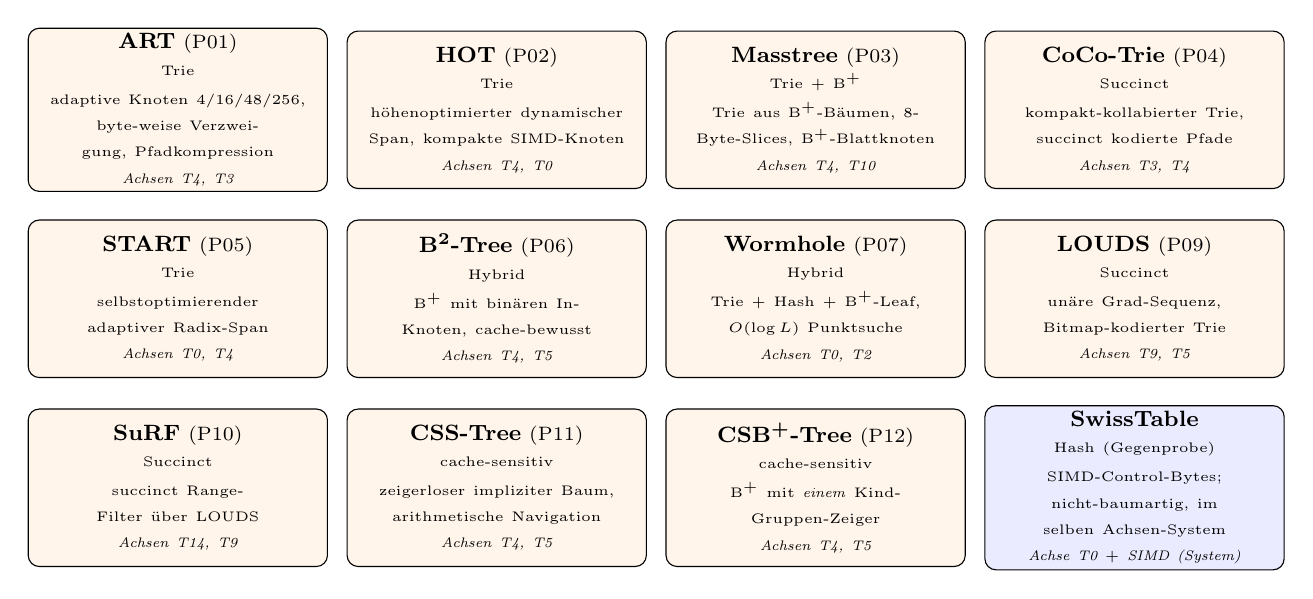
\begin{tikzpicture}[font=\footnotesize,
  so/.style={draw,rounded corners,fill=orange!8,minimum width=3.8cm,minimum height=2.0cm,text width=3.55cm,align=center,inner sep=2pt}]
  \node[so] (a1) at (0,0){\textbf{ART} {\scriptsize(P01)}\\{\tiny Trie}\\[1pt]{\tiny adaptive Knoten 4/16/48/256, byte-weise Verzweigung, Pfadkompression}\\{\tiny\itshape Achsen T4, T3}};
  \node[so] (a2) at (4.05,0){\textbf{HOT} {\scriptsize(P02)}\\{\tiny Trie}\\[1pt]{\tiny höhenoptimierter dynamischer Span, kompakte SIMD-Knoten}\\{\tiny\itshape Achsen T4, T0}};
  \node[so] (a3) at (8.1,0){\textbf{Masstree} {\scriptsize(P03)}\\{\tiny Trie $+$ B\textsuperscript{+}}\\[1pt]{\tiny Trie aus B\textsuperscript{+}-Bäumen, 8-Byte-Slices, B\textsuperscript{+}-Blattknoten}\\{\tiny\itshape Achsen T4, T10}};
  \node[so] (a4) at (12.15,0){\textbf{CoCo-Trie} {\scriptsize(P04)}\\{\tiny Succinct}\\[1pt]{\tiny kompakt-kollabierter Trie, succinct kodierte Pfade}\\{\tiny\itshape Achsen T3, T4}};
  \node[so] (b1) at (0,-2.4){\textbf{START} {\scriptsize(P05)}\\{\tiny Trie}\\[1pt]{\tiny selbstoptimierender adaptiver Radix-Span}\\{\tiny\itshape Achsen T0, T4}};
  \node[so] (b2) at (4.05,-2.4){\textbf{B\textsuperscript{2}-Tree} {\scriptsize(P06)}\\{\tiny Hybrid}\\[1pt]{\tiny B\textsuperscript{+} mit binären In-Knoten, cache-bewusst}\\{\tiny\itshape Achsen T4, T5}};
  \node[so] (b3) at (8.1,-2.4){\textbf{Wormhole} {\scriptsize(P07)}\\{\tiny Hybrid}\\[1pt]{\tiny Trie $+$ Hash $+$ B\textsuperscript{+}-Leaf, $O(\log L)$ Punktsuche}\\{\tiny\itshape Achsen T0, T2}};
  \node[so] (b4) at (12.15,-2.4){\textbf{LOUDS} {\scriptsize(P09)}\\{\tiny Succinct}\\[1pt]{\tiny unäre Grad-Sequenz, Bitmap-kodierter Trie}\\{\tiny\itshape Achsen T9, T5}};
  \node[so] (c1) at (0,-4.8){\textbf{SuRF} {\scriptsize(P10)}\\{\tiny Succinct}\\[1pt]{\tiny succinct Range-Filter über LOUDS}\\{\tiny\itshape Achsen T14, T9}};
  \node[so] (c2) at (4.05,-4.8){\textbf{CSS-Tree} {\scriptsize(P11)}\\{\tiny cache-sensitiv}\\[1pt]{\tiny zeigerloser impliziter Baum, arithmetische Navigation}\\{\tiny\itshape Achsen T4, T5}};
  \node[so] (c3) at (8.1,-4.8){\textbf{CSB\textsuperscript{+}-Tree} {\scriptsize(P12)}\\{\tiny cache-sensitiv}\\[1pt]{\tiny B\textsuperscript{+} mit \emph{einem} Kind-Gruppen-Zeiger}\\{\tiny\itshape Achsen T4, T5}};
  \node[draw,rounded corners,fill=blue!8,minimum width=3.8cm,minimum height=2.0cm,text width=3.55cm,align=center,inner sep=2pt] (c4) at (12.15,-4.8){\textbf{SwissTable}\\{\tiny Hash (Gegenprobe)}\\[1pt]{\tiny SIMD-Control-Bytes; nicht-baumartig, im selben Achsen-System}\\{\tiny\itshape Achse T0 $+$ SIMD (System)}};
\end{tikzpicture}
\caption{Galerie der wichtigsten rekonstruierten Suchstrukturen: je Verfahren (mit Paper-ID) seine Herkunfts-Klasse, die charakteristische Struktur-Idee und die Achsen, an denen es seinen Hauptbeitrag leistet. Trie-, Hybrid-, succinct- und cache-sensitive Verfahren stehen neben einer nicht-baumartigen Hash-Gegenprobe (SwissTable) --- alle als Punkte im selben Achsen-Entwurfsraum. Die vollständige Achsen-Sezierung führt Tabelle~\ref{tab:axes-overview}.}\label{fig:sota-gallery}
\end{figure}
\end{nurlang}
\begin{nurkurz}
Die Veröffentlichungen entstammen sechs \emph{Herkunfts-Clustern}, die der Einordnung jedes Lebewesens dienen,
bevor es in seine Organe zerlegt wird: die \emph{Trie-Familie} mit ART (P01)~\cite{leis2013art}, HOT
(P02)~\cite{binna2018hot}, Masstree (P03)~\cite{mao2012masstree}, CoCo-Trie (P04)~\cite{boffa2024coco}, START
(P05)~\cite{fent2020start}, LOUDS (P09)~\cite{jacobson1989louds} und SuRF (P10)~\cite{zhang2018surf}; die
\emph{Hybrid- und B\textsuperscript{+}-Familie} mit B\textsuperscript{2}-Baum (P06)~\cite{schmeisser2022b2tree},
Wormhole (P07)~\cite{wu2019wormhole} und den CSS-, CSB\textsuperscript{+}- und Hankins-Bäumen
(P11--P13)~\cite{rao1999css,rao2000csb,hankins2003nodesize}; die \emph{Layout-Theorie} mit Samuel
(P14)~\cite{samuel2005procaware}, Graefe/Larson (P15)~\cite{graefe2001btree}, Bender et
al.\ (P16/P17)~\cite{bender2000cobtree,bender2005coboblivious} und Saikkonen/Soisalon-Soininen
(P18/P19)~\cite{saikkonen2008multilevel,saikkonen2016layout}; das \emph{Prefetching} mit \emph{B-Trees Are Back}
(P20)~\cite{mueller2025btreesback}, Chen et al.\ (P21/P22)~\cite{chen2001prefetch,chen2002fractal}, Khan
(P23)~\cite{khan2010adaptive}, Naderan-Tahan (P24)~\cite{naderan2016adaptivefilter}, Mahling
(P25)~\cite{mahling2025hotpath}, Zhang (P26/P27)~\cite{zhang2024pathprefix,zhang2025hierarchical} und Kuehn
(P28)~\cite{kuehn2023bplustree}; die \emph{Synchronisation} mit OLC-ART (P08)~\cite{leis2016olc}, RCU
(P29)~\cite{mckenney2001rcu} und Hazard-Pointern (P30)~\cite{michael2004hazard}; die \emph{TU-Dresden-Linie}
mit Ungethüm (P31)~\cite{ungethuem2017survey}, Schmidt (P32)~\cite{schmidt2025hbm} und VAMPIR
(P33)~\cite{berthold2023vampir}. Der \emph{Allokator-Korpus} (A01--A23) spannt von
dlmalloc~\cite{lea1996dlmalloc}, Hoard~\cite{berger2000hoard}, Slab/Magazines/Vmem~\cite{bonwick1994slab,bonwick2001vmem}
und Michaels lock-freier Allokation~\cite{michael2004lockfree} über mimalloc~\cite{leijen2019mimalloc},
jemalloc~\cite{evans2006jemalloc}, TCMalloc~\cite{ghemawat2005tcmalloc}, snmalloc~\cite{lietar2019snmalloc},
scalloc~\cite{aigner2015scalloc}, rpmalloc~\cite{jansson2017rpmalloc} und lrmalloc~\cite{leite2018lrmalloc} bis
zu CAMA~\cite{herter2011cama}, NUMAlloc~\cite{yang2023numalloc}, StarMalloc~\cite{reitz2024starmalloc} und
PIM-malloc~\cite{pimmalloc2026}.
\end{nurkurz}

\begin{nurlang}
Für jeden SOTA-Algorithmus (\emph{State of the Art} --- der Stand der Technik aus
Abschnitt~\ref{sec:overview}) und jeden Allokator hält ein Profil-XML die Achsen-Belegung fest: die
Organ-Belegung (\texttt{node}, \texttt{traversal}, \texttt{value\_handle}, \texttt{concurrency},
\texttt{allocator}, \texttt{prefetch}, \texttt{layout}, \texttt{reclamation}), die Prüfling-Build-Achse
\texttt{page} und --- getrennt davon, weil keine Organ-Belegung --- die Ziel-ISA (\texttt{isa},
System-Sphäre) und die Telemetrie (\texttt{telemetry}, Mess-Tooling); dazu eine Schlüssel-Wert-Signatur
und einen optionalen \texttt{<expected\_workload>}-Tag, der die Mess-Heuristik überschreibt
(Tabelle~\ref{tab:sota-profiles}).
\end{nurlang}
\begin{nurkurz}
Für jeden SOTA-Algorithmus (\emph{State of the Art} --- der Stand der Technik aus
Abschnitt~\ref{sec:overview}) und jeden Allokator hält ein Profil-XML die Achsen-Belegung fest: die
Organ-Belegung (\texttt{node}, \texttt{traversal}, \texttt{value\_handle}, \texttt{concurrency},
\texttt{allocator}, \texttt{prefetch}, \texttt{layout}, \texttt{reclamation}), die Prüfling-Build-Achse
\texttt{page} und --- getrennt davon, weil keine Organ-Belegung --- die Ziel-ISA (\texttt{isa},
System-Sphäre) und die Telemetrie (\texttt{telemetry}, Mess-Tooling); dazu eine Schlüssel-Wert-Signatur
und einen optionalen \texttt{<expected\_workload>}-Tag, der die Mess-Heuristik überschreibt.
\end{nurkurz}

%% INTERN-272: KA-011
Für jede der 33~Korpus-Arbeiten und jeden der 23~Allokatoren liegt ein Profil-XML mit
\texttt{<expected\_workload>}-Tag vor. Die Profile sind zweierlei Typs --- der Typ ist im Profil-XML
markiert und in der Prüflings-Registry der Cache-Engine übersetzungsstatisch verankert: 30
\emph{Vollprofile} beschreiben eigenständige Suchentwürfe vollständig; drei \emph{abstrakte Profile}
gehen nur seziert ein --- das optimistische Lock-Coupling von ART~\cite{leis2016olc} als
Nebenläufigkeits-Organ, die succinct LOUDS-Repräsentation~\cite{jacobson1989louds} als
Speicher-Layout-Organ (u.\,a.\ in SuRF~\cite{zhang2018surf}) und das Profiling-Werkzeug
VAMPIR~\cite{berthold2023vampir} als Mess-Technologie. Ein abstraktes Profil stellt einige Organe selbst
und überlässt die übrigen dem Standard-Baukasten; es ist derselbe Typ, dem der Prüfling PRT-ART
entspricht (Abschnitt~\ref{sec:prtart-demo}), und Vollprofile fremder Prüflinge sind auf demselben Weg
eingliederbar. Der Entwurf sieht je Achse eine getrennte Permutation über
\emph{Profil-Ranges} vor --- ein Wertebereich je Achse statt eines Einzelwerts; die persistierten
Profile enthalten je Achse einen Einzelwert, die Bereichs-Permutation ist nicht implementiert.

\begin{nurlang}
\begin{table}[!htbp]
  \caption{SOTA-Profile (33: 30 Vollprofile, 3 abstrakte) mit Workload-Affinität}\label{tab:sota-profiles}
  \centering\small
  \begin{tabular}{llll}
    \toprule
    \textbf{Profil} & \textbf{Paper-Ref.} & \textbf{Typ} & \textbf{expected\_workload} \\
    \midrule
    art & P01 (Leis 2013) & voll & YCSB\_C \\
    hot & P02 (Binna 2018) & voll & YCSB\_C \\
    masstree & P03 (Mao 2012) & voll & YCSB\_A \\
    coco\_trie & P04 (Boffa 2024) & voll & YCSB\_C \\
    start & P05 (Fent 2020) & voll & YCSB\_C \\
    b2tree & P06 (Schmeisser 2022) & voll & YCSB\_E \\
    wormhole & P07 (Wu 2019) & voll & YCSB\_A \\
    olc & P08 (Leis 2016) & abstrakt & YCSB\_B \\
    louds & P09 (Jacobson 1989) & abstrakt & YCSB\_A \\
    surf & P10 (Zhang 2018) & voll & YCSB\_A \\
    css\_tree & P11 (Rao/Ross 1999) & voll & YCSB\_C \\
    csb\_tree & P12 (Rao/Ross 2000) & voll & YCSB\_E \\
    hankins & P13 (Hankins 2003) & voll & YCSB\_C \\
    samuel & P14 (Samuel 2005) & voll & YCSB\_C \\
    graefe & P15 (Graefe 2001) & voll & YCSB\_C \\
    bender\_treelayout & P16 (Bender 2002) & voll & YCSB\_C \\
    bender\_cacheoblivious & P17 (Bender 2005) & voll & YCSB\_C \\
    saikkonen\_multilevel & P18 (Saikkonen 2008) & voll & YCSB\_E \\
    saikkonen\_layoutinvariant & P19 (Saikkonen 2016) & voll & YCSB\_E \\
    btreesareback & P20 (Mueller 2025) & voll & YCSB\_E \\
    chen\_prefetch & P21 (Chen 2001) & voll & YCSB\_A \\
    chen\_fractal & P22 (Chen 2002) & voll & YCSB\_A \\
    khan\_adaptive & P23 (Khan 2010) & voll & YCSB\_A \\
    naderan\_tahan & P24 (Naderan-Tahan 2016) & voll & YCSB\_A \\
    mahling & P25 (Mahling 2025) & voll & YCSB\_E \\
    zhang\_fgcs & P26 (Zhang 2024) & voll & YCSB\_A \\
    zhang\_asplos & P27 (Zhang 2025) & voll & YCSB\_A \\
    kuehn & P28 (Kuehn 2023) & voll & YCSB\_C \\
    rcu & P29 (McKenney 2001) & voll & YCSB\_B \\
    hazard\_pointers & P30 (Michael 2004) & voll & YCSB\_B \\
    ungethuem & P31 (Ungethuem 2017) & voll & YCSB\_C \\
    to\_stride & P32 (Schmidt 2025) & voll & YCSB\_C \\
    vampir & P33 (Berthold 2023) & abstrakt & YCSB\_B \\
    \bottomrule
  \end{tabular}

  \smallskip
  {\footnotesize \texttt{expected\_workload} = YCSB-Workload-Klasse (A/B/C/E/F); Typ: voll = Vollprofil eines
  eigenständigen Suchentwurfs, abstrakt = abstraktes Profil, das nur seziert eingeht.\par}
\end{table}
\end{nurlang}

Über alle 33 Profile hinweg verteilen sich diese Affinitäten auf 13$\times$~YCSB\_C (leselastig),
10$\times$~YCSB\_A (Zipf-verteiltes Lesen und Aktualisieren), 6$\times$~YCSB\_E (Bereichs-Scans) und
4$\times$~YCSB\_B (95/5 Lesen/Aktualisieren); PRT-ART selbst ist in seinem Prüflings-Profil mit YCSB\_F
(Read-Modify-Write, für die DensityTracker-Aktualisierungen) getaggt.

Der Kern-Befund dieser Lastprofil-Analyse ist ein systematischer \emph{Bias}: Jede Veröffentlichung wählt
das Lastprofil, unter dem ihr eigener Entwurf am besten abschneidet. Statische, read-only-orientierte
Tries und Filter (HOT~\cite{binna2018hot}, CoCo~\cite{boffa2024coco},
B\textsuperscript{2}-Baum~\cite{schmeisser2022b2tree}, SuRF~\cite{zhang2018surf}, CSS~\cite{rao1999css})
rahmen \enquote{build-once, 100\,\% positive Lookups} und meiden Aktualisierungen; komprimierte Tries und
Filter (CoCo, B\textsuperscript{2}-Baum, SuRF) machen den Negativ-Anfrage-Anteil zur Primärachse, weil sie
bei Misses früh abbrechen; zipfian-zentrierte Arbeiten (B-Trees Are Back~\cite{mueller2025btreesback},
Mahling~\cite{mahling2025hotpath}, Kuehn~\cite{kuehn2023bplustree}) begünstigen cache-bewusste
Reordering-Layouts; schreib- und nebenläufigkeits-lastige Arbeiten (ART~\cite{leis2013art},
Masstree~\cite{mao2012masstree}, Wormhole~\cite{wu2019wormhole}, OLC-ART~\cite{leis2016olc},
RCU~\cite{mckenney2001rcu}) treten umgekehrt nur dort an, wo statische Strukturen versagen; und prefetch-
bzw.\ hardware-nahe Arbeiten (CSB\textsuperscript{+}~\cite{rao2000csb}, Chen~\cite{chen2001prefetch},
Schmidt~\cite{schmidt2025hbm}) vermessen über Knotengröße und Prefetch eher Cache und TLB als die
Algorithmus-Logik. Vierzehn der Veröffentlichungen steuern kein distinktes Lastprofil zum Katalog bei ---
teils Survey-, Theorie- und Hardware-Arbeiten ohne eigenes Index-Lastprofil, teils Arbeiten, deren
Custom-Microbenchmarks in bereits katalogisierten Profilen aufgehen. Erst wenn \emph{alle} Lastprofile
gegen \emph{alle} Lebewesen-Binaries (und die Container-Hüllen, Abschnitt~\ref{sec:anatomy-levels})
laufen --- der Workload als dynamische Achse
(Kapitel~\ref{ch:eval}) ---, lässt sich ein Vorteil, der nur unter dem selbstgewählten Lastprofil besteht,
sichtbar machen und bias-reduzierte Vergleichbarkeit gewinnen.

\begin{nurlang}
Schließlich erscheinen auch die Güte-Kriterien wissenschaftlichen Messens (vgl.\ die Definitions-Klassen in Abschnitt~\ref{sec:measurement-system})
als konkrete Technologien.\ \emph{Hardware-Performance-Zähler} (PMC, über \texttt{perf})~\cite{demelo2010perf}
sind nahezu universell und liefern Cache-Miss-Raten, dTLB-Misses, Branch-Misses und IPC/CPI --- die
Mehrzahl der Arbeiten P01--P28 berichtet solche Zähler ---; \emph{Profiler}
wie OTF2/VAMPIR~\cite{berthold2023vampir} und VTune~\cite{reinders2005vtune} erheben trace-basierte
Laufzeitprofile, \emph{Simulatoren} wie gem5~\cite{binkert2011gem5} liefern hardware-genaue Schätzungen, wo
reale Zähler fehlen (so P25 Mahling~\cite{mahling2025hotpath}, P27
Zhang~\cite{zhang2025hierarchical}), und das \emph{HdrHistogram}~\cite{tene_hdrhistogram} erhebt die Latenz-Perzentile
(p50/p95/p99). Auf der Erhebung baut die Auswertung auf: Statt arithmetischer Mittel werden Median und
Perzentile berichtet, Unterschiede mit dem verteilungsfreien \emph{Mann-Whitney-U-Test}~\cite{mann1947utest}
(mit Holm-Korrektur der Familienfehlerrate~\cite{holm1979sequential}) auf Signifikanz geprüft und über das Effektmaß
\emph{Cliff's~$\delta$}~\cite{cliff1993dominance} quantifiziert, den Empfehlungen für wissenschaftliches
Benchmarking~\cite{hoefler2015benchmarking} folgend. Eine eigene methodische Linie bildet die hardware-nahe
Messmethodik der TU Dresden (Habich-Gruppe): Ungethüm et al.~\cite{ungethuem2017survey} systematisieren die
Hardware-Optimierungen für Datenbank-Maschinen, Schmidt et al.~\cite{schmidt2025hbm} vermessen Stride- gegen
Sequenz-Zugriffe auf HBM mit dTLB- und L2/L3-Zählern, und VAMPIR~\cite{berthold2023vampir} profiliert nicht-funktionale Eigenschaften
heterogener Speicher. Aus all diesen Technologien ergibt sich der Satz der Mess-Kategorien ---
Cache-Line-Auslastung, Cache-Misses (L1/L2/L3), dTLB-Misses, Speicher-Fußabdruck, Branch-Misses,
IPC/CPI, Latenz (Mittel und Perzentile p50--p999), Durchsatz, Energie und Fill-Buffer-Auslastung ---,
deren zeit- und observer-basierte Teilmenge der eigene Apparat bereits auflöst (Wall-Clock,
HdrHistogram in der nachgelagerten Auswertung, Per-Achsen-Observer, die Statistik-Triade aus
Median/Perzentilen, Signifikanztest und Effektmaß, die Zwei-Phasen-Operationsschleife und das
Konformitäts-Gatter gegen \texttt{std::map}),
während die zählerbasierten PMC-Kategorien im Mess-Pfad verbindlich eingebaut sind und ihre Belegung je
Mikroarchitektur an einen Ereignis-Katalog gebunden ist (Abschnitt~\ref{sec:axis-triad}); die
vollständige Mess-Architektur entwickeln das Mess-System (Abschnitt~\ref{sec:measurement-system})
und Kapitel~\ref{ch:eval}.
\end{nurlang}
\begin{nurkurz}
Schließlich erscheinen auch die Güte-Kriterien wissenschaftlichen Messens (vgl.\ die Definitions-Klassen in
Abschnitt~\ref{sec:measurement-system}) als konkrete Technologien: \emph{Hardware-Performance-Zähler} (PMC, über
\texttt{perf})~\cite{demelo2010perf} liefern IPC/CPI, Cache-Miss-Raten, dTLB-Misses und Branch-Misses;
\emph{Profiler} wie OTF2/VAMPIR~\cite{berthold2023vampir} und VTune~\cite{reinders2005vtune} erheben
trace-basierte Laufzeitprofile, \emph{Simulatoren} wie gem5~\cite{binkert2011gem5} liefern hardware-genaue
Schätzungen, wo reale Zähler fehlen, und das \emph{HdrHistogram}~\cite{tene_hdrhistogram} erhebt die
Latenz-Perzentile. Berichtet werden Median und Perzentile statt arithmetischer Mittel, Unterschiede mit dem
verteilungsfreien \emph{Mann-Whitney-U-Test}~\cite{mann1947utest} (Holm-Korrektur~\cite{holm1979sequential})
geprüft und über \emph{Cliff's~$\delta$}~\cite{cliff1993dominance} quantifiziert~\cite{hoefler2015benchmarking};
eine eigene Linie bildet die hardware-nahe Messmethodik der TU
Dresden~\cite{ungethuem2017survey,schmidt2025hbm,berthold2023vampir}. Aus all diesen Technologien ergibt sich
der Satz der Mess-Kategorien ---
Cache-Line-Auslastung, Cache-Misses (L1/L2/L3), dTLB-Misses, Speicher-Fußabdruck, Branch-Misses,
IPC/CPI, Latenz (Mittel und Perzentile p50--p999), Durchsatz, Energie und Fill-Buffer-Auslastung ---,
deren zeit- und observer-basierte Teilmenge der eigene Apparat bereits auflöst, während die zählerbasierten
PMC-Kategorien im Mess-Pfad verbindlich eingebaut und je Mikroarchitektur an einen Ereignis-Katalog gebunden
sind (Abschnitt~\ref{sec:axis-triad}); die vollständige Mess-Architektur entwickeln das Mess-System
(Abschnitt~\ref{sec:measurement-system}) und Kapitel~\ref{ch:eval}.
\end{nurkurz}

%% INTERN-272: KA-012
\section{Lösungskonzept: das Anatomie-Modell}\label{sec:anatomy-model}
Aus der dialektischen Aneignung des Standes der Technik ergibt sich das Lösungskonzept dieser Arbeit;
dieser Abschnitt entwickelt es als \emph{Anatomie-Modell} und definiert dabei die Begrifflichkeiten und
konzeptionellen Spezialkonstrukte, auf denen die folgenden Abschnitte aufbauen.

\begin{nurlang}
\subsection{Achsen-Komposition und die Lebewesen-Metapher}\label{sec:anatomy-metaphor}
Die zentrale Idee ist, einen Algorithmus nicht als Monolith zu behandeln, sondern als \emph{Komposition
orthogonaler Achsen} --- jede Achse eine Teilentscheidung eines Cache-bewussten bzw. System-bewussten Index (wie Seiten
angeordnet werden, wie Knoten verzweigen, wie Speicher alloziert wird). Ein konkreter Algorithmus ist dann
ein Punkt im kartesischen Produkt aller Achsen, ein Stand-der-Technik-Entwurf eine explizite
Konfiguration. Entscheidend ist die \emph{modulare Austauschbarkeit}: Eine neue Achsen-Variante lässt sich
isoliert untersuchen --- ihr Effekt je Achse \emph{und} für den ganzen Algorithmus messen ---, ohne die
übrigen neu zu implementieren; genau das löst das Trennbarkeits-Problem, da der Beitrag jedes Bestandteils
bei sonst fixierten Achsen isoliert messbar wird. Dass diese Austauschbarkeit modular ist, zeigt sich im
Code: Die Referenz-Kompositionen von ART und PRT-ART unterscheiden sich in genau einer Achse, der
Pfadkompression (Abschnitt~\ref{sec:prtart-demo}). Diese Zerlegung beruht auf der Beobachtung gemeinsamer Belange unterschiedlicher Suchalgorithmen und Veröffentlichungen, sowie der Vergleichbarkeit der Ziele unterschiedlicher Suchalgorithmen und kann daher durch eine Metapher getragen werden. Erstens
teilen Suchalgorithmen im großen Bild dieselbe \emph{Baum-Anatomie} in unterschiedlicher Ausprägung ---
von ausgewogenen Suchbäumen über Tries und Radix-Bäume bis zu eigenentwickelten Konstrukten; selbst eine
sortierte Schlüssel-Wert-Liste ist streng genommen ein einzelnes Blatt eines Baumes, dessen Werte über
Verweise weiter auf Daten-Blätter zeigen. Die Haupt-Differenzen zwischen den Algorithmus-Ausprägungen belaufen sich dadurch auf die Auffächerung der Knoten, die Baum-Tiefe, die Baum-Filter und Regelwerke, und die Implementierungs-Details der Serialisierung von Speicherseiten, Such-Seiten und Baum-Knoten. Die Baum-Struktur ist damit universell über alle Suchalgorithmus-Architekturen hinweg und bildet die Zeichenfläche, auf der die Achsen platziert werden.
\end{nurlang}
\begin{nurkurz}
\subsection{Achsen-Komposition und die Lebewesen-Metapher}\label{sec:anatomy-metaphor}
Die zentrale Idee ist, einen Algorithmus nicht als Monolith zu behandeln, sondern als \emph{Komposition
orthogonaler Achsen} --- jede Achse eine Teilentscheidung eines cache- bzw.\ system-bewussten Index. Ein
konkreter Algorithmus ist dann ein Punkt im kartesischen Produkt aller Achsen, ein Stand-der-Technik-Entwurf
eine explizite Konfiguration. Entscheidend ist die \emph{modulare Austauschbarkeit}: Eine neue Achsen-Variante
lässt sich isoliert untersuchen, ohne die übrigen neu zu implementieren --- genau das löst das
Trennbarkeits-Problem, da der Beitrag jedes Bestandteils bei sonst fixierten Achsen isoliert messbar wird; im
Code unterscheiden sich die Referenz-Kompositionen von ART und PRT-ART in genau einer Achse, der
Pfadkompression (Abschnitt~\ref{sec:prtart-demo}). Getragen wird die Zerlegung davon, dass Suchalgorithmen im
großen Bild dieselbe \emph{Baum-Anatomie} teilen --- selbst eine sortierte Schlüssel-Wert-Liste ist ein
einzelnes Blatt eines Baumes ---; die Baum-Struktur ist die universelle Zeichenfläche, auf der die Achsen
platziert werden.
\end{nurkurz}

\begin{nurlang}
%% INTERN-272: KA-013
Nicht-baumartige Suchverfahren --- etwa die Hash-Gegenprobe aus Abschnitt~\ref{sec:sota-instances} ---
bleiben dieselbe Gattung mit eingeschränktem Profil, denn eine eigene Gattung entstünde erst, wenn sich
der Basis-Achsen-Satz grundlegend unterschiede: Auch eine Hash-Tabelle ist ein Baum, der von der Wurzel
seines Interfaces über eine Auffächerung an Hashes sucht --- nur der Kern-Algorithmus des Knotens ist ein
anderer. Deshalb gehört jedes Verfahren, das einen Schlüssel in einen Wert übersetzt, gleich wie, zur
Gattung Map und ihrem Genus \texttt{SearchAlgorithm} (Abschnitt~\ref{sec:anatomy-levels}). Zweitens
fasst eine anschauliche Metapher einen konkreten Algorithmus als \emph{Lebewesen} auf, dessen
\emph{Organe} die Achsen sind. Die Metapher ist kanonisch besetzt: Das \emph{Blut} ist das flüssige
Organ, das alle Organ-Achsen verbindet und im Planer zu einer Übersetzungszeit-Konfiguration verdichtet
wird; die System-Achsen sind der \emph{Lebensraum} (der Planet) des Tiers mit den Möglichkeiten und
Ressourcen, die sich dort finden; die Mess-Achsen sind die Ausstattung des \emph{Labors}, in dem das
Tier untersucht wird (Abbildung~\ref{fig:anatomy-bridge}). Ein Tier kann ohne Messung sehr gut leben,
aber nur das gesündeste Tier soll in den produktiven Einsatz gegeben werden --- und jedes Tier soll
bestmöglich an seinen Lebensraum angepasst sein: Besitzt es eine Eigenschaft nicht, kann es diesen Teil
seines Lebensraums (die Hardware) nicht zu seinem Vorteil nutzen; oder die Messung ergründet, dass seine
Spezialisierung gar nicht auf diesen Lebensraum ausgelegt sein sollte, weil sie die Qualität des Tiers
dort negativ beeinflusst --- ein Affe soll klettern und ein Fisch schwimmen, nicht umgekehrt, weil
unterschiedliche Zielstellungen zu unterschiedlichen Entwürfen geführt haben. Diese Metapher ist dem
Hintergrund des Autors in der Biomedizinischen Technik geschuldet und soll die Analyse durch
Bildhaftigkeit vereinfachen; ab hier arbeitet die Arbeit durchgängig mit diesem Modell.
\end{nurlang}
\begin{nurkurz}
Nicht-baumartige Suchverfahren --- etwa die Hash-Gegenprobe aus Abschnitt~\ref{sec:sota-instances} ---
bleiben dieselbe Gattung mit eingeschränktem Profil: Auch eine Hash-Tabelle ist ein Baum, der von der Wurzel
seines Interfaces über eine Auffächerung an Hashes sucht; jedes Verfahren, das einen Schlüssel in einen Wert
übersetzt, gehört zur Gattung Map und ihrem Genus \texttt{SearchAlgorithm} (Abschnitt~\ref{sec:anatomy-levels}).
Eine anschauliche Metapher fasst einen Algorithmus als \emph{Lebewesen} auf, dessen \emph{Organe} die Achsen
sind; sie ist kanonisch besetzt: Das \emph{Blut} ist das flüssige Organ, das alle Organ-Achsen verbindet und im
Planer zu einer Übersetzungszeit-Konfiguration verdichtet wird; die System-Achsen sind der \emph{Lebensraum} des
Tiers mit seinen Ressourcen; die Mess-Achsen sind die Ausstattung des \emph{Labors}, in dem das Tier untersucht
wird. Die Permutation der Achsen ist in dieser Lesart ein Organ-Austausch, der neue Komposit-Algorithmen mit
unbekanntem Cache-Line-Verhalten erzeugt; die Organe selbst werden aus dem Stand der Technik gewonnen
(Abschnitt~\ref{sec:overview}), dessen Entwurfsbausteine in orthogonale Achsen zerlegt und in einer gemeinsamen
Achsen-Matrix gesammelt werden. Software-technisch ist eine Achse ein Feature, die \emph{Gattung} die
Feature-\emph{Kern}-Komposition (der gemeinsame Interface-Kern aller Genera) und das \emph{Genus} die
Feature-\emph{Spezial}-Komposition (das reale Tier-Interface über den Kern hinaus,
Abschnitt~\ref{sec:anatomy-levels})~\cite{apel2013feature,batory1992hierarchical}; ab hier arbeitet die Arbeit
durchgängig mit diesem Modell.
\end{nurkurz}

\begin{nurlang}
\begin{figure}[htbp]\centering
\begin{tikzpicture}[font=\footnotesize, align=center, >=Stealth,
  organism/.style={draw, rounded corners, minimum width=2.8cm, minimum height=3.4cm, fill=red!4},
  org/.style={draw, circle, fill=red!15, minimum size=0.78cm, inner sep=0pt, font=\scriptsize},
  axis/.style={draw, rounded corners, fill=green!10, minimum width=2.2cm, minimum height=0.55cm, font=\scriptsize},
  habitat/.style={draw, rounded corners, fill=yellow!16, minimum height=0.7cm, text width=7.8cm, font=\scriptsize}]
  \node[organism] (body) at (0,-0.1){};
  \node[font=\scriptsize] at (0,1.95){\textbf{Lebewesen} (Anatomie)};
  \node[org] (o1) at (0,0.9){Herz};
  \node[org] (o2) at (-0.65,-0.1){Lunge};
  \node[org] (o3) at (0.65,-0.1){Leber};
  \node[org] (o4) at (0,-1.1){Niere};
  \draw[->,very thick] (1.7,-0.1) -- (3.0,-0.1) node[midway,above,font=\scriptsize]{Organ $\equiv$ Achse};
  \node[font=\scriptsize] at (5.4,1.95){\textbf{Suchalgorithmus} (Achsen)};
  \node[axis] (a1) at (5.4,0.9){Traversal};
  \node[axis] (a2) at (5.4,0.2){Layout};
  \node[axis] (a3) at (5.4,-0.5){Allokator};
  \node[axis] (a4) at (5.4,-1.2){Prefetch};
  \draw[red!60!black,thick] (4.15,1.15) -- (4.15,-1.45);
  \foreach \y in {0.9,0.2,-0.5,-1.2}{\draw[red!60!black,thick] (4.15,\y) -- (4.3,\y);}
  \node[font=\tiny,text=red!60!black,rotate=90] at (3.95,-0.15){Blut $=$ Verbindung der Organ-Achsen};
  \node[habitat,minimum width=8.2cm] (hab) at (2.7,-2.45){\textbf{Lebensraum} (System-Achsen): der Planet mit seinen Ressourcen --- immer präsent, keiner Gattung zugehörig};
  \node[draw, fill=blue!8, font=\scriptsize, align=center] (mess) at (8.3,-0.15){Mess-System\\(\enquote{Labor})};
  \draw[->,blue] (mess) -- (a1); \draw[->,blue] (mess) -- (a2);
  \draw[->,blue] (mess) -- (a3); \draw[->,blue] (mess) -- (a4);
\end{tikzpicture}
\caption{Die Anatomie-Brücke: wie ein Lebewesen aus zusammenwirkenden Organen besteht, ist ein Suchalgorithmus eine Komposition von Achsen-Organen; das Blut verbindet die Organ-Achsen, der Lebensraum (die System-Achsen) trägt das Tier, und das Mess-System übernimmt die Rolle des Labors, das jedes Organ einzeln vermisst.}\label{fig:anatomy-bridge}
\end{figure}
\end{nurlang}

\begin{nurlang}
Die Permutation der Achsen ist in dieser Lesart ein Organ-Austausch: Der Austausch von Organen zwischen
Lebewesen erzeugt neue Komposit-Algorithmen mit bisher unbekanntem Cache-Line-Verhalten. Die Organe selbst
werden aus dem Stand der Technik gewonnen --- die Entwurfsbausteine der bekannten Verfahren
(Abschnitt~\ref{sec:overview}) werden in orthogonale Achsen zerlegt und in einer gemeinsamen
Achsen-Matrix gesammelt, sodass jede Achse die Beiträge des gesamten Korpus erntet
(Abbildung~\ref{fig:synth}).
\begin{figure}[htbp]\centering
\begin{tikzpicture}[font=\footnotesize,>=Stealth,align=center,
  paper/.style={draw,rounded corners,fill=orange!12,minimum width=1.8cm,minimum height=0.52cm},
  ax/.style={draw,fill=green!12,minimum width=2.2cm,minimum height=0.5cm,font=\scriptsize}]
  \node[font=\scriptsize,text=gray] at (0,2.95){Stand der Technik};
  \node[paper] (p1) at (0,2.2){ART};
  \node[paper] (p2) at (0,1.5){HOT};
  \node[paper] (p3) at (0,0.8){SuRF};
  \node[paper] (p4) at (0,0.1){Masstree};
  \node[paper] (p5) at (0,-0.6){Bw-Baum};
  \node[font=\scriptsize,text=gray] at (5.6,2.95){die Achsen-Matrix};
  \node[ax] (x1) at (5.6,2.2){Knotentyp};
  \node[ax] (x2) at (5.6,1.5){Layout};
  \node[ax] (x3) at (5.6,0.8){Allokator};
  \node[ax] (x4) at (5.6,0.1){Prefetch};
  \node[ax] (x5) at (5.6,-0.6){Nebenläufigkeit};
  \foreach \p in {p1,p2,p3,p4,p5}{\foreach \x in {x1,x2,x3,x4,x5}{\draw[gray!22,->] (\p.east)--(\x.west);}}
  \node[align=center,font=\scriptsize] at (2.8,-1.7){jeder Algorithmus zerfällt in Achsen-Belegungen ---\\die Matrix erntet die Bausteine des gesamten Korpus};
\end{tikzpicture}
\caption{Synthese Stand der Technik $\to$ Achsen: die Entwurfsbausteine der bekannten Verfahren werden in orthogonale Achsen zerlegt; jede Achse sammelt die Beiträge des gesamten Korpus --- die Umkehrung von Abbildung~\ref{fig:design-space} (dort ist ein Algorithmus ein Punkt, hier eine Achse ein Sammelbecken).}\label{fig:synth}
\end{figure}
\end{nurlang}

\begin{nurlang}
Die so gewonnene \emph{Anatomie} ist mehr als die Aufzählung der Organe: Sie ist ihre \emph{Verdrahtung}.
Jedes Organ exportiert ein generalisiertes Interface, über das die übrigen seine Dienste nutzen, ohne
dessen konkrete Belegung zu kennen --- so stellt das Allokations-Organ ein gemeinsames
Allokations-Interface bereit, das Knoten-Layout, Wert-Ablage und Serialisierung für ihre
Speicheranforderungen verwenden (Abbildung~\ref{fig:axis-organ}); der Hub dieser Verdrahtung ist im Code
das Speicher-Organ \texttt{LayoutAwareChunkedStore}, das Knotentyp, Layout und Allokator komponiert
(\enquote{Speicher-Organ-Interface} ist der Konzeptname, kein Code-Typ). Die Nutzungs-Regeln sind weit
gefasst: Eine Achse darf fremde Achsen-Interfaces nutzen, sich selbst rekursiv aufrufen und andere
Gattungen verwenden --- die Such-Gattung greift in ihren Interface-Funktionen auf Achsen zu und verwendet
eigene Container-Genera, und Teile des Achsen-Pools werden für die Container wiederverwendet
(Abschnitt~\ref{sec:measurement-system}). Software-technisch ist dies die \emph{Feature-Interaktion}
feature-orientierter Software-Produktlinien~\cite{apel2013feature,batory1992hierarchical}.
\end{nurlang}
\begin{nurkurz}
Die so gewonnene \emph{Anatomie} ist mehr als die Aufzählung der Organe: Sie ist ihre \emph{Verdrahtung}. Jedes
Organ exportiert ein generalisiertes Interface, über das die übrigen seine Dienste nutzen, ohne dessen Belegung
zu kennen; der Hub ist im Code das Speicher-Organ \texttt{LayoutAwareChunkedStore}, das Knotentyp, Layout und
Allokator komponiert. Die Nutzungs-Regeln sind weit gefasst --- eine Achse darf fremde Achsen-Interfaces nutzen,
sich rekursiv aufrufen und andere Gattungen verwenden, Teile des Achsen-Pools werden für die Container
wiederverwendet (Abschnitt~\ref{sec:measurement-system}) ---; software-technisch ist dies die
\emph{Feature-Interaktion} feature-orientierter Produktlinien~\cite{apel2013feature,batory1992hierarchical}.
\end{nurkurz}

\begin{nurlang}
%% INTERN-272: KA-014
Eine Achse entspricht einem Feature, ein Lebewesen einer Feature-Komposition. Die \emph{Gattung} ist die
Feature-\emph{Kern}-Komposition: der gemeinsame Interface-Kern, den alle Genera einer Gattung teilen und
der in der Metaprogrammierung über alle Variationen hinweg gleich verwendet wird --- so wie verschiedene
Map-Kategorien (Hash-Map, flache Map) einen gemeinsamen Kern an Interface-Funktionen teilen; für die
Container-Gattung besteht dieser Kern aus Identität, Achsen-Beobachtung und Größe. Das \emph{Genus}
(Alias: Tier-Unterklasse, Abschnitt~\ref{sec:anatomy-levels}) ist die Feature-\emph{Spezial}-Komposition:
das reale Tier-Interface über den Kern hinaus --- \texttt{SearchAlgorithm}, \texttt{Set},
\texttt{Sequence}, \texttt{Adapter}, \texttt{View} und \texttt{FunctionInterfaceReroute} --- und damit
eine statische Feature-Set-Definition. Die Anatomie ist die Verdrahtung zwischen den Features. Welche
Achse welche nutzt, zeigt der Inter-Organ-Nutzungs-Graph (Abbildung~\ref{fig:usage}).
\begin{figure}[htbp]\centering
\begin{tikzpicture}[font=\footnotesize,>=Stealth,align=center,
  organ/.style={draw,circle,minimum size=1.05cm,fill=green!7,inner sep=1pt}]
  \node[organ,fill=blue!12,minimum size=1.3cm] (store) at (0,0){Speicher-\\organ};
  \node[organ] (alloc) at (-3.0,1.5){Allokator};
  \node[organ] (node) at (-3.0,0){Knotentyp};
  \node[organ] (layout) at (-3.0,-1.5){Layout};
  \node[organ] (search) at (3.0,0){Suche};
  \node[organ,fill=gray!8] (obs) at (2.8,-2.3){Telemetrie};
  \draw[->,thick,blue] (alloc)--(store);
  \draw[->,thick,blue] (node)--(store);
  \draw[->,thick,blue] (layout)--(store);
  \draw[->,thick,blue] (store)--(search) node[midway,above,font=\scriptsize,text=blue]{muss};
  \draw[->,dashed,gray] (store)--(obs) node[midway,right,font=\scriptsize]{kann};
  \node[font=\scriptsize,blue] at (0,-1.6){Speicher-Organ-Interface\\{\tiny (\texttt{LayoutAwareChunkedStore})}};
\end{tikzpicture}
\caption{Achse $=$ Organ, Anatomie $=$ Verdrahtung: das Speicher-Organ (Komposition aus Knotentyp, Layout und Allokator) exportiert ein generalisiertes Speicher-Organ-Interface (im Code \texttt{LayoutAwareChunkedStore}), über das die Suche läuft (durchgezogen, \emph{verpflichtend}); weitere Organe wie die Telemetrie \emph{können} es über optionale Beobachter-Hooks nutzen (gestrichelt, \emph{optional}), müssen aber nicht.}\label{fig:axis-organ}
\end{figure}
\end{nurlang}

\begin{nurlang}
Setzt man diese paarweisen \emph{Organ-Kopplungen} --- eine Organ-Kopplung ist die wechselseitige
Abhängigkeit zweier Achsen, bei der die eine das Interface der anderen nutzt (verpflichtend oder
optional) oder deren zulässige Belegungen einschränkt; Teilfrage FF1.b (Abschnitt~\ref{sec:rqs})
spricht sie für Knotentyp, SIMD und Pfadkompression an --- über alle Organe zusammen, entsteht ein
gerichteter Inter-Organ-Nutzungs-Graph.
\begin{figure}[htbp]\centering
%% INTERN-272: KA-015
\begin{tikzpicture}[font=\footnotesize,>=Stealth,align=center,
  org/.style={draw,rounded corners,fill=green!8,minimum width=2.1cm,minimum height=0.66cm,font=\scriptsize},
  hub/.style={draw,rounded corners,fill=blue!12,minimum width=3.2cm,minimum height=1.15cm,text width=3.0cm,align=center,font=\scriptsize,very thick}]
  \node[hub] (store) at (0,0){\textbf{Speicher-Organ}\\\texttt{Layout\-Aware\-Chunked\-Store}\\{\scriptsize T4\,$\oplus$\,T5\,$\oplus$\,T6}};
  \node[org] (alloc) at (-4.1,1.4){Allokator (T6)};
  \node[org] (node) at (-4.1,0){Knotentyp (T4)};
  \node[org] (layout) at (-4.1,-1.4){Layout (T5)};
  \node[org] (search) at (4.1,0){Suche (T0)};
  \node[org] (prefetch) at (4.1,1.4){Prefetch (T7)};
  \node[org,fill=gray!8] (obs) at (4.1,-1.4){Telemetrie (Mess)};
  \node[org,fill=gray!6] (conc) at (0,-2.6){Nebenläufigkeit (T8)};
  \draw[->,very thick,blue] (alloc)--(store);
  \draw[->,very thick,blue] (node)--(store);
  \draw[->,very thick,blue] (layout)--(store);
  \draw[->,very thick,blue] (store)--(search) node[midway,above,font=\scriptsize]{muss};
  \draw[->,dashed,gray] (store)--(prefetch) node[midway,above,font=\scriptsize]{kann};
  \draw[->,dashed,gray] (store)--(obs);
  \draw[->,dotted,gray] (conc)--(store);
\end{tikzpicture}
\caption{Inter-Organ-Nutzungs-Graph (\enquote{welche Achse nutzt welche}): Es gibt genau \emph{einen}
kanonischen Hub --- das Speicher-Organ \texttt{LayoutAwareChunkedStore}, das Knotentyp~(T4), Layout~(T5)
und Allokator~(T6) komponiert.\ \emph{Verpflichtend} (durchgezogen) konsumiert der Store diese drei Achsen,
und die Suche~(T0) läuft über ihn. Alle übrigen Kopplungen sind \emph{optional} (gestrichelt): Prefetch~(T7)
und die Telemetrie (Mess-Instrumentierung, Abschnitt~\ref{sec:axis-triad}) lesen den Store nur über \texttt{requires}-gegatete Beobachter-Hooks --- eine Achse
\emph{kann} fremde Interfaces nutzen, \emph{muss} aber nicht. Die Kopplung der Nebenläufigkeit~(T8) an den
Store ist nicht angebunden (gepunktet). Der Graph ist eine Beispiel-Verdrahtung des Speicher-Organs,
keine im Code ausgewertete Struktur.}\label{fig:usage}
\end{figure}
%% INTERN-272: KA-016
\subsection{Das Drei-Ebenen-Modell und die vier Gattungen}\label{sec:anatomy-levels}
Diese Organe sind in \emph{eine} Architektur eingebettet --- eine einzige, in sich geschlossene Hierarchie
ohne Parallel-Bäume. An ihrer Wurzel steht die \texttt{ExecutionEngine} als gemeinsame, ausmessbare
Abstraktion über allem Messbaren --- sie bleibt bestehen, weil \texttt{IExecutionEngine} die
gemeinsame messbare Wurzel bildet und \texttt{IAnatomyBase} die anatomie-tragende Sicht unmittelbar darunter;
darunter lassen sich drei Ebenen unterscheiden: die \emph{Gattung} als nach außen sichtbares
Algorithmus-Interface (das \emph{Prüf-Dock}), darunter das \emph{Genus} (Alias: \emph{Tier-Unterklasse})
mit festem Achsensatz, darunter die \emph{Organe} selbst (Abbildung~\ref{fig:three-levels})\@. Die
Ebenen-Trennung ist an der ABI-Grenze ablesbar: Jede Tier-Binary exportiert zwei buchstabengleiche
C-Symbole, die Gattung und Genus ohne Instanz beantworten, wobei die Gattung nicht als zweites Datum
gepflegt, sondern aus dem Genus abgeleitet wird --- der Lader ermittelt die Gattung so über ein
gattungsunabhängiges Symbol, ohne sie vorab zu kennen\@. \enquote{Lebewesen} und \texttt{SearchAlgorithm} bezeichnen denselben
Gegenstand --- Metapher und technischer Begriff ---; die Anatomie ist kein zweites Modell, sondern der
\emph{Körper} dieses Lebewesens: die feste Komposition seiner achtzehn Achsen-Organe.
\begin{figure}[htbp]\centering
\begin{tikzpicture}[font=\footnotesize,>=Stealth,align=center,
  box/.style={draw,rounded corners,inner sep=3pt,minimum height=0.7cm},
  lvl/.style={font=\scriptsize,text=gray,anchor=east,align=right}]
  \node[box] (root) at (1.1,0){\texttt{IExecutionEngine} (messbare Wurzel) $\to$ \texttt{IAnatomyBase} (anatomie-tragend)};
  \node[lvl] at (-5.1,-1.6){Ebene 1: Gattung\\{\tiny Feature-Kern-Komposition}};
  \node[box] (sa) at (-3.0,-1.6){Map};
  \node[box] (co) at (0,-1.6){Container};
  \node[box] (gr) at (2.6,-1.6){Graph};
  \node[box] (ha) at (5.3,-1.6){HeuristikAdapter};
  \node[lvl] at (-5.1,-3.3){Ebene 2: Genus\\{\tiny Feature-Spezial-Komposition}};
  \node[box] (tier) at (-3.0,-3.3){\texttt{SearchAlgorithm}\\{\scriptsize Säugetier, 18 Organ-Achsen}};
  \node[box] (cont2) at (0,-3.3){\texttt{Set}, \texttt{Sequence},\\\texttt{Adapter}, \texttt{View}};
  \node[box,dashed,fill=gray!8] (gr2) at (2.6,-3.3){kein Genus\\{\scriptsize implementiert}};
  \node[box] (ha2) at (5.3,-3.3){\texttt{FunctionInterface}-\\\texttt{Reroute}};
  \node[lvl] at (-5.1,-4.75){Ebene 3: Organe};
  \node[box,fill=green!8] (org) at (-3.0,-4.75){Achsen T0--T17};
  \node[box,fill=green!8] (org2) at (0,-4.75){Achsen des Pools};
  \draw[->] (root)--(sa);\draw[->] (root)--(co);\draw[->] (root)--(gr);\draw[->] (root)--(ha);
  \draw[->] (sa)--(tier);\draw[->] (co)--(cont2);\draw[->,dashed] (gr)--(gr2);\draw[->] (ha)--(ha2);
  \draw[->] (tier)--(org);\draw[->] (cont2)--(org2);
\end{tikzpicture}
\caption{Das Drei-Ebenen-Modell: Gattung (Ebene~1, Außen-Interface, Feature-Kern-Komposition) $\to$ Genus (Ebene~2, fester Achsen-Satz, Feature-Spezial-Komposition) $\to$ Organe/Achsen (Ebene~3). Vier Gattungen: \texttt{Map} besitzt als einziges Genus \texttt{SearchAlgorithm} das \enquote{Säugetier} mit den achtzehn Organ-Achsen; \texttt{Container} die Genera Set/Sequence/Adapter/View, die aus demselben Achsen-Pool gebildet werden; \texttt{Graph} ist als Interface angelegt, ein Genus ist nicht implementiert; \texttt{HeuristikAdapter} besitzt das Reroute-Genus \texttt{FunctionInterfaceReroute} des Hybrid-Tiers.}\label{fig:three-levels}
\end{figure}
\end{nurlang}
\begin{nurkurz}
Setzt man die paarweisen \emph{Organ-Kopplungen} --- eine Organ-Kopplung ist die wechselseitige Abhängigkeit
zweier Achsen, bei der die eine das Interface der anderen nutzt (verpflichtend oder optional) oder deren
zulässige Belegungen einschränkt; Teilfrage FF1.b (Abschnitt~\ref{sec:rqs}) spricht sie für Knotentyp, SIMD
und Pfadkompression an --- über alle Organe zusammen, entsteht ein gerichteter Inter-Organ-Nutzungs-Graph mit
dem Speicher-Organ als einzigem kanonischen Hub.
\subsection{Das Drei-Ebenen-Modell und die vier Gattungen}\label{sec:anatomy-levels}
Diese Organe sind in \emph{eine} Architektur eingebettet --- eine einzige Hierarchie ohne Parallel-Bäume. An
ihrer Wurzel steht die \texttt{ExecutionEngine} als gemeinsame, ausmessbare Abstraktion
(\texttt{IExecutionEngine} als messbare Wurzel, \texttt{IAnatomyBase} als anatomie-tragende Sicht darunter);
darunter liegen drei Ebenen: die \emph{Gattung} als nach außen sichtbares Algorithmus-Interface (das
\emph{Prüf-Dock}), das \emph{Genus} (Alias: \emph{Tier-Unterklasse}) mit festem Achsensatz und die
\emph{Organe} selbst (Abbildung~\ref{fig:three-levels}). Die Ebenen-Trennung ist an der ABI-Grenze ablesbar:
Jede Tier-Binary exportiert zwei buchstabengleiche C-Symbole, die Gattung und Genus ohne Instanz beantworten,
wobei die Gattung aus dem Genus abgeleitet wird.\ \enquote{Lebewesen} und \texttt{SearchAlgorithm} bezeichnen
denselben Gegenstand; die Anatomie ist der \emph{Körper} dieses Lebewesens, die feste Komposition seiner
achtzehn Achsen-Organe.
\begin{figure}[htbp]\centering
\begin{tikzpicture}[font=\footnotesize,>=Stealth,align=center,
  box/.style={draw,rounded corners,inner sep=3pt,minimum height=0.7cm},
  lvl/.style={font=\scriptsize,text=gray,anchor=east,align=right}]
  \node[box] (root) at (1.1,0){\texttt{IExecutionEngine} (messbare Wurzel) $\to$ \texttt{IAnatomyBase} (anatomie-tragend)};
  \node[lvl] at (-5.1,-1.6){Ebene 1: Gattung\\{\tiny Feature-Kern-Komposition}};
  \node[box] (sa) at (-3.0,-1.6){Map};
  \node[box] (co) at (0,-1.6){Container};
  \node[box] (gr) at (2.6,-1.6){Graph};
  \node[box] (ha) at (5.3,-1.6){HeuristikAdapter};
  \node[lvl] at (-5.1,-3.3){Ebene 2: Genus\\{\tiny Feature-Spezial-Komposition}};
  \node[box] (tier) at (-3.0,-3.3){\texttt{SearchAlgorithm}\\{\scriptsize Säugetier, 18 Organ-Achsen}};
  \node[box] (cont2) at (0,-3.3){\texttt{Set}, \texttt{Sequence},\\\texttt{Adapter}, \texttt{View}};
  \node[box,dashed,fill=gray!8] (gr2) at (2.6,-3.3){kein Genus\\{\scriptsize implementiert}};
  \node[box] (ha2) at (5.3,-3.3){\texttt{FunctionInterface}-\\\texttt{Reroute}};
  \node[lvl] at (-5.1,-4.75){Ebene 3: Organe};
  \node[box,fill=green!8] (org) at (-3.0,-4.75){Achsen T0--T17};
  \node[box,fill=green!8] (org2) at (0,-4.75){Achsen des Pools};
  \draw[->] (root)--(sa);\draw[->] (root)--(co);\draw[->] (root)--(gr);\draw[->] (root)--(ha);
  \draw[->] (sa)--(tier);\draw[->] (co)--(cont2);\draw[->,dashed] (gr)--(gr2);\draw[->] (ha)--(ha2);
  \draw[->] (tier)--(org);\draw[->] (cont2)--(org2);
\end{tikzpicture}
\caption{Das Drei-Ebenen-Modell: Gattung (Ebene~1, Außen-Interface, Feature-Kern-Komposition) $\to$ Genus (Ebene~2, fester Achsen-Satz, Feature-Spezial-Komposition) $\to$ Organe/Achsen (Ebene~3). Vier Gattungen: \texttt{Map} besitzt als einziges Genus \texttt{SearchAlgorithm} das \enquote{Säugetier} mit den achtzehn Organ-Achsen; \texttt{Container} die Genera Set/Sequence/Adapter/View, die aus demselben Achsen-Pool gebildet werden; \texttt{Graph} ist als Interface angelegt, ein Genus ist nicht implementiert; \texttt{HeuristikAdapter} besitzt das Reroute-Genus \texttt{FunctionInterfaceReroute} des Hybrid-Tiers.}\label{fig:three-levels}
\end{figure}
\end{nurkurz}

\begin{nurlang}
Auf der obersten Ebene stehen vier Gattungen. Die \texttt{Map}-Gattung --- das
schlüssel-wert-orientierte Prüf-Dock und der Fokus dieser Arbeit --- besitzt als einziges Genus
\texttt{SearchAlgorithm} das volle Achtzehn-Achsen-\enquote{Säugetier}; die \texttt{Container}-Gattung
(schlüsselloser Speicher) fächert in die Genera Set, Sequence, Adapter und View auf, die ebenfalls aus
Achsen des gemeinsamen Pools gebildet werden und deren Slot-Zahl je Genus übersetzungsstatisch
festliegt; die \texttt{Graph}-Gattung ist als Interface angelegt, ein Genus ist nicht implementiert; und
die \texttt{HeuristikAdapter}-Gattung besitzt das Reroute-Genus \texttt{FunctionInterfaceReroute} --- die
Gattung des Hybrid-Tiers (Abschnitt~\ref{sec:heuristics-modes}), das per Metaprogrammierung die
Interfaces einer Gattung samt Genus erbt und Anfragen an die eigentlichen Tier-Binaries durchstellt;
Klassifikation (welcher Art das Reroute ist) und Durchstellung (das geerbte Ziel-Genus, das die Binary
nach außen meldet) liegen dabei auf getrennten Ebenen (Abbildung~\ref{fig:genera}). Merkregel:
\enquote{Adapter} ohne Präfix meint immer das Container-Genus; die Hybrid-Gattung heißt stets
HeuristikAdapter. Das dort als Wurzel gezeigte Reich \enquote{Animalia} ($\equiv$ \texttt{IAnatomyBase})
ist die anatomie-tragende Sicht unmittelbar unterhalb der messbaren Wurzel \texttt{IExecutionEngine} aus
Abbildung~\ref{fig:three-levels}; die Code-Trennung der beiden Interfaces vertieft Kapitel~\ref{ch:impl}.
Nicht-baumartige Verfahren erfordern so keine eigene Gattung, sondern belegen ein eingeschränktes
Achsen-Subset derselben Gattung.
\begin{figure}[htbp]\centering
%% INTERN-272: KA-017
\begin{tikzpicture}[font=\footnotesize,>=Stealth,align=center,
  gen/.style={draw,rounded corners,fill=blue!10,minimum width=2.5cm,minimum height=0.66cm,font=\bfseries\footnotesize},
  sub/.style={draw,fill=green!8,minimum width=2.8cm,minimum height=0.62cm,font=\scriptsize},
  tbd/.style={draw,dashed,fill=gray!12,minimum width=2.5cm,minimum height=0.7cm,font=\scriptsize},
  band/.style={draw,rounded corners,fill=orange!9,minimum width=13.6cm,minimum height=1.05cm,text width=13.2cm,align=left,font=\scriptsize}]
  \node[draw,rounded corners,fill=red!6,font=\footnotesize] (root) at (1.3,1.6){Reich \enquote{Animalia} ($\equiv$ \texttt{IAnatomyBase}, anatomie-tragend)};
  %% INTERN-272: KA-018
  \node[gen] (g1) at (-4.0,0){Map};
  \node[gen] (g2) at (0.6,0){Container};
  \node[gen] (g3) at (4.3,0){Graph};
  \node[gen,minimum width=2.9cm] (g4) at (7.4,0){HeuristikAdapter};
  \draw[->] (root)--(g1); \draw[->] (root)--(g2); \draw[->] (root)--(g3); \draw[->] (root)--(g4);
  %% INTERN-272: KA-019
  \node[sub,fill=green!18] (s1) at (-4.0,-1.3){\textbf{Säugetier} $=$ \texttt{SearchAlgorithm}\\{\scriptsize \texttt{map}-Hülle $\cdot$ 18 Organ-Achsen}};
  \node[sub,anchor=west] (c1) at (-1.2,-1.15){Vogel $=$ Set {\scriptsize(\texttt{set})}};
  \node[sub,anchor=west] (c2) at (-1.2,-1.95){Reptil $=$ Sequence {\scriptsize(\texttt{vector})}};
  \node[sub,anchor=west] (c3) at (-1.2,-2.75){Wirbelloses $=$ Adapter {\scriptsize(\texttt{stack})}};
  \node[sub,anchor=west] (c4) at (-1.2,-3.55){Pflanze $=$ View {\scriptsize(\texttt{span})}};
  \node[tbd,text width=2.4cm,anchor=north] (gr1) at (4.3,-0.7){Interface angelegt,\\{\scriptsize kein Genus}\\{\scriptsize implementiert}};
  \node[sub,minimum width=2.9cm,text width=2.9cm,anchor=north] (h1) at (7.4,-0.7){\texttt{FunctionInterface}\\\texttt{Reroute}\\{\scriptsize Hybrid-Tier:}\\{\scriptsize geerbtes Ziel-Genus}};
  \draw[->] (g1)--(s1); \draw[->,dashed] (g3)--(gr1); \draw[->] (g4)--(h1);
  %% INTERN-272: KA-020
  \draw (g2.south) -- ++(0,-0.3) -| (-1.5,-3.55);
  \draw[->] (-1.5,0 |- c1.west) -- (c1.west); \draw[->] (-1.5,0 |- c2.west) -- (c2.west);
  \draw[->] (-1.5,0 |- c3.west) -- (c3.west); \draw[->] (-1.5,0 |- c4.west) -- (c4.west);
  %% INTERN-272: KA-021
  \node[band] (l3) at (1.3,-4.75){\textbf{Ebene 3 --- Organe:} die 18 Organ-Achsen (Knotentyp, Layout, Allokator, Prefetch, \dots) \emph{permutieren}; die Container-Genera bilden sich aus demselben Achsen-Pool.};
  \node[band] (l4) at (1.3,-6.15){\textbf{Ebene 4 --- konkretes Tier:} eine Belegung \emph{aller} Achsen $=$ ein Individuum (ART, HOT, Masstree, SuRF, START, Wormhole, \dots; 30 Vollprofile) --- ein abstraktes Profil (PRT-ART, OLC, LOUDS, VAMPIR) belegt nur einige Achsen selbst.};
  \node[band,fill=orange!20,very thick,minimum height=1.25cm] (l5) at (1.3,-7.7){\textbf{Ebene 5 --- Tier-Binary (Träger-Stufe):} je Permutation kompiliert zu \texttt{comdare\_perm\_\-<fp>.dll}\,/\,\texttt{.so}, verfeinert um die Prüfling-Build-Achse Seitentyp; die Plattform stempeln die drei System-Achsen, die Mess-Wahl die Mess-Zeile; jede Tier-Binary bietet die drei Interface-Flächen (Abbildung~\ref{fig:traeger-flaechen}).};
  \draw[->,thick] (s1.south) -- (s1.south |- l3.north);
  \draw[->,thick] (l3.south) -- (l4.north); \draw[->,thick] (l4.south) -- (l5.north);
\end{tikzpicture}
\caption[Die vier Gattungen und die Tier-Hierarchie bis zum kompilierten Binary]{Die Gattungs-/Tier-Hierarchie über fünf Ebenen. \texttt{Map}, \texttt{Container}, \texttt{Graph} und \texttt{HeuristikAdapter} sind die vier \emph{Gattungen} (Ebene~1, Außen-Interface). Jede Gattung beherbergt ihre \emph{eigenen} Genera (Ebene~2, Alias Tier-Unterklassen): \texttt{Map} ausschließlich das \enquote{Säugetier} (Genus \texttt{SearchAlgorithm}, volle Achtzehn-Achsen-Anatomie), \texttt{Container} jedes \emph{nicht}-Säugetier-Genus (Vogel/Reptil/Wirbelloses/Pflanze $=$ Set/Sequence/Adapter/View), \texttt{Graph} ein angelegtes Interface ohne implementiertes Genus, \texttt{HeuristikAdapter} das Reroute-Genus des Hybrid-Tiers. Der Säugetier-Ast ist bis zum Individuum ausgezogen: die achtzehn Achsen-Organe (Ebene~3) permutieren zu einer konkreten Achsen-Komposition $=$ einem konkreten Tier (Ebene~4, z.\,B.\ ART, HOT, Masstree), das je Permutation als eigenständige Tier-Binary kompiliert wird (Ebene~5, die Träger-Stufe der Tier-Binary, zusätzlich verfeinert um die Prüfling-Build-Achse Seitentyp und plattform-gestempelt durch die drei System-Achsen, Abschnitt~\ref{sec:axis-triad})\@. \emph{Jede Tier-Binary ist damit ein eigenes Tier mit einem tatsächlichen Binary-Genus-Interface und drei Interface-Flächen}; die Hierarchie reicht von der Gattung bis zur einzelnen kompilierten Permutation. Vgl.\ das verdichtete Modell in Abbildung~\ref{fig:three-levels}.}\label{fig:genera}
\end{figure}
\end{nurlang}
\begin{nurkurz}
Auf der obersten Ebene stehen vier Gattungen (Abbildung~\ref{fig:genera}): \texttt{Map} --- das
schlüssel-wert-orientierte Prüf-Dock und der Fokus dieser Arbeit --- besitzt als einziges Genus
\texttt{SearchAlgorithm} das volle Achtzehn-Achsen-\enquote{Säugetier}; \texttt{Container} fächert in die Genera
Set, Sequence, Adapter und View auf, die aus demselben Achsen-Pool gebildet werden; \texttt{Graph} ist als
Interface angelegt, ein Genus ist nicht implementiert; \texttt{HeuristikAdapter} besitzt das Reroute-Genus
\texttt{FunctionInterfaceReroute} --- die Gattung des Hybrid-Tiers (Abschnitt~\ref{sec:heuristics-modes}), das
per Metaprogrammierung die Interfaces einer Gattung samt Genus erbt und Anfragen an die eigentlichen
Tier-Binaries durchstellt. Merkregel: \enquote{Adapter} ohne Präfix meint immer das Container-Genus, die
Hybrid-Gattung heißt stets HeuristikAdapter; das Reich \enquote{Animalia} ($\equiv$ \texttt{IAnatomyBase}) ist
die anatomie-tragende Sicht unterhalb der messbaren Wurzel \texttt{IExecutionEngine} (Kapitel~\ref{ch:impl}).
Nicht-baumartige Verfahren erfordern so keine eigene Gattung, sondern belegen ein eingeschränktes
Achsen-Subset derselben Gattung.
\begin{figure}[htbp]\centering
%% INTERN-272: KA-017
\begin{tikzpicture}[font=\footnotesize,>=Stealth,align=center,
  gen/.style={draw,rounded corners,fill=blue!10,minimum width=2.5cm,minimum height=0.66cm,font=\bfseries\footnotesize},
  sub/.style={draw,fill=green!8,minimum width=2.8cm,minimum height=0.62cm,font=\scriptsize},
  tbd/.style={draw,dashed,fill=gray!12,minimum width=2.5cm,minimum height=0.7cm,font=\scriptsize},
  band/.style={draw,rounded corners,fill=orange!9,minimum width=13.6cm,minimum height=1.05cm,text width=13.2cm,align=left,font=\scriptsize}]
  \node[draw,rounded corners,fill=red!6,font=\footnotesize] (root) at (1.3,1.6){Reich \enquote{Animalia} ($\equiv$ \texttt{IAnatomyBase}, anatomie-tragend)};
  %% INTERN-272: KA-018
  \node[gen] (g1) at (-4.0,0){Map};
  \node[gen] (g2) at (0.6,0){Container};
  \node[gen] (g3) at (4.3,0){Graph};
  \node[gen,minimum width=2.9cm] (g4) at (7.4,0){HeuristikAdapter};
  \draw[->] (root)--(g1); \draw[->] (root)--(g2); \draw[->] (root)--(g3); \draw[->] (root)--(g4);
  %% INTERN-272: KA-019
  \node[sub,fill=green!18] (s1) at (-4.0,-1.3){\textbf{Säugetier} $=$ \texttt{SearchAlgorithm}\\{\scriptsize \texttt{map}-Hülle $\cdot$ 18 Organ-Achsen}};
  \node[sub,anchor=west] (c1) at (-1.2,-1.15){Vogel $=$ Set {\scriptsize(\texttt{set})}};
  \node[sub,anchor=west] (c2) at (-1.2,-1.95){Reptil $=$ Sequence {\scriptsize(\texttt{vector})}};
  \node[sub,anchor=west] (c3) at (-1.2,-2.75){Wirbelloses $=$ Adapter {\scriptsize(\texttt{stack})}};
  \node[sub,anchor=west] (c4) at (-1.2,-3.55){Pflanze $=$ View {\scriptsize(\texttt{span})}};
  \node[tbd,text width=2.4cm,anchor=north] (gr1) at (4.3,-0.7){Interface angelegt,\\{\scriptsize kein Genus}\\{\scriptsize implementiert}};
  \node[sub,minimum width=2.9cm,text width=2.9cm,anchor=north] (h1) at (7.4,-0.7){\texttt{FunctionInterface}\\\texttt{Reroute}\\{\scriptsize Hybrid-Tier:}\\{\scriptsize geerbtes Ziel-Genus}};
  \draw[->] (g1)--(s1); \draw[->,dashed] (g3)--(gr1); \draw[->] (g4)--(h1);
  %% INTERN-272: KA-020
  \draw (g2.south) -- ++(0,-0.3) -| (-1.5,-3.55);
  \draw[->] (-1.5,0 |- c1.west) -- (c1.west); \draw[->] (-1.5,0 |- c2.west) -- (c2.west);
  \draw[->] (-1.5,0 |- c3.west) -- (c3.west); \draw[->] (-1.5,0 |- c4.west) -- (c4.west);
  %% INTERN-272: KA-021
  \node[band] (l3) at (1.3,-4.75){\textbf{Ebene 3 --- Organe:} die 18 Organ-Achsen (Knotentyp, Layout, Allokator, Prefetch, \dots) \emph{permutieren}; die Container-Genera bilden sich aus demselben Achsen-Pool.};
  \node[band] (l4) at (1.3,-6.15){\textbf{Ebene 4 --- konkretes Tier:} eine Belegung \emph{aller} Achsen $=$ ein Individuum (ART, HOT, Masstree, SuRF, START, Wormhole, \dots; 30 Vollprofile) --- ein abstraktes Profil (PRT-ART, OLC, LOUDS, VAMPIR) belegt nur einige Achsen selbst.};
  \node[band,fill=orange!20,very thick,minimum height=1.25cm] (l5) at (1.3,-7.7){\textbf{Ebene 5 --- Tier-Binary (Träger-Stufe):} je Permutation kompiliert zu \texttt{comdare\_perm\_\-<fp>.dll}\,/\,\texttt{.so}, verfeinert um die Prüfling-Build-Achse Seitentyp; die Plattform stempeln die drei System-Achsen, die Mess-Wahl die Mess-Zeile; jede Tier-Binary bietet die drei Interface-Flächen (Abbildung~\ref{fig:traeger-flaechen}).};
  \draw[->,thick] (s1.south) -- (s1.south |- l3.north);
  \draw[->,thick] (l3.south) -- (l4.north); \draw[->,thick] (l4.south) -- (l5.north);
\end{tikzpicture}
\caption[Die vier Gattungen und die Tier-Hierarchie bis zum kompilierten Binary]{Die Gattungs-/Tier-Hierarchie über fünf Ebenen. \texttt{Map}, \texttt{Container}, \texttt{Graph} und \texttt{HeuristikAdapter} sind die vier \emph{Gattungen} (Ebene~1, Außen-Interface). Jede Gattung beherbergt ihre \emph{eigenen} Genera (Ebene~2, Alias Tier-Unterklassen): \texttt{Map} ausschließlich das \enquote{Säugetier} (Genus \texttt{SearchAlgorithm}, volle Achtzehn-Achsen-Anatomie), \texttt{Container} jedes \emph{nicht}-Säugetier-Genus (Vogel/Reptil/Wirbelloses/Pflanze $=$ Set/Sequence/Adapter/View), \texttt{Graph} ein angelegtes Interface ohne implementiertes Genus, \texttt{HeuristikAdapter} das Reroute-Genus des Hybrid-Tiers. Der Säugetier-Ast ist bis zum Individuum ausgezogen: die achtzehn Achsen-Organe (Ebene~3) permutieren zu einer konkreten Achsen-Komposition $=$ einem konkreten Tier (Ebene~4, z.\,B.\ ART, HOT, Masstree), das je Permutation als eigenständige Tier-Binary kompiliert wird (Ebene~5, die Träger-Stufe der Tier-Binary, zusätzlich verfeinert um die Prüfling-Build-Achse Seitentyp und plattform-gestempelt durch die drei System-Achsen, Abschnitt~\ref{sec:axis-triad})\@. \emph{Jede Tier-Binary ist damit ein eigenes Tier mit einem tatsächlichen Binary-Genus-Interface und drei Interface-Flächen}; die Hierarchie reicht von der Gattung bis zur einzelnen kompilierten Permutation. Vgl.\ das verdichtete Modell in Abbildung~\ref{fig:three-levels}.}\label{fig:genera}
\end{figure}
\end{nurkurz}

\begin{nurlang}
Die Anatomie wird von vier \emph{Träger-Stufen} (carrier stages) getragen: dem Planer, dem
\emph{CacheEngineBuilder} (CEB) --- dem Messwerkzeug, das der Planer je Ziel-Plattform und Mess-Aufgabe
erzeugt ---, der Tier-Binary und der Hybrid-Tier-Binary. Der Planer löst die Anwender-XML gegen die drei
Angebots-Kataloge auf und wählt zu seiner Laufzeit die Mess-Achsen; der CEB enthält diese Mess-Wahl
einkompiliert, kennt die Plattform und permutiert System- und Organ-Achsen zu Tier-Binaries; die
Tier-Binary enthält die Organ-Permutation; die Hybrid-Tier-Binary führt zusätzlich ihre angeschlossenen
Tiere. Die Steuerung sitzt im Planer, und die Kette der Freigaben ist gerichtet: Die Mess-Achsen
bestimmen den CEB-Typ, der CEB definiert die System-Achsen und gibt den Bau-Raum frei, und dieser Raum
permutiert System- und Organ-Achsen zur Tier-Binary. Keine Stufe durchläuft dabei Schichten --- jede
enthält ihre Schicht fest einkompiliert; nur die Konfiguration wandert von der XML bis zur fertigen
Tier-Binary. Die Interfaces der Träger folgen einem Drei-Flächen-Modell: Fläche~1 ist das
Genus-Interface einer Tier-Binary (Laufzeit, Abstract Factory), Fläche~2 der Stempel (Übersetzungszeit,
ABI-stabil, Abschnitt~\ref{sec:stamp-model}), Fläche~3 der Mess-Durchstich (\texttt{IMessVisitor}), der
die Messung als eigene Naht quert, damit Gattungs- und Genus-Interfaces unverändert bleiben. An Tier-
und Hybrid-Tier-Binary sind alle drei Flächen ausgeprägt; Planer und CEB besitzen die Stempel-Fläche, und
der CEB führt zusätzlich seine eigene Mess-Gate-Belegung, deren Deckung gegen die Tier-Gates (CEB aus,
Tier an) durch einen Test belegt ist. Die Verträge zwischen Planer, CEB, Tier und Hybrid sind je Stufe lokal
auf sieben Stempel-Interfaces verteilt --- eine Gesamt-Selbst-Version führt nur der Planer, Mess- und
System-Zeile führen CEB, Tier und Hybrid, die Organ-Zeile führen nur Tier und Hybrid (die Absenz beim
CEB ist die statische Sperre \enquote{der CEB führt keine Organ-Achsen}), Fingerprint und
Gesamt-Stempel führen alle vier, und die angeschlossenen Tiere führt nur der Hybrid
(Abbildung~\ref{fig:traeger-flaechen}).
\begin{figure}[htbp]\centering
\begin{tikzpicture}[font=\scriptsize,>=Stealth,align=center,
  tr/.style={draw,rounded corners,fill=blue!10,minimum width=2.1cm,minimum height=0.6cm,text width=1.9cm,font=\bfseries\scriptsize},
  p/.style={draw,fill=green!18,minimum width=2.1cm,minimum height=0.48cm,text width=1.95cm,font=\tiny},
  v/.style={draw,fill=gray!10,minimum width=2.1cm,minimum height=0.48cm,text width=1.95cm,text=gray,font=\tiny},
  fl/.style={draw,rounded corners,fill=orange!10,minimum width=2.1cm,minimum height=1.25cm,text width=1.95cm,font=\tiny},
  lab/.style={anchor=east,font=\scriptsize}]
  %% INTERN-272: KA-022
  \node[tr] (t0) at (0,0){Planer};
  \node[tr] (t1) at (2.5,0){CEB};
  \node[tr] (t2) at (5.0,0){Tier-Binary};
  \node[tr] (t3) at (7.5,0){Hybrid-Tier};
  \draw[->,thick] (t0)--(t1); \draw[->,thick] (t1)--(t2); \draw[->,thick] (t2)--(t3);
  \node[font=\tiny,anchor=south] at (3.75,0.38){Konfiguration wandert: XML $\to$ Planer $\to$ CEB $\to$ Tier $\to$ Hybrid (keine Stufe durchläuft Schichten)};
  %% INTERN-272: KA-023
  \node[lab] at (-1.2,-0.75){\texttt{version\_xyz}};
  \node[p] at (0,-0.75){Pflicht}; \node[v] at (2.5,-0.75){verboten}; \node[v] at (5.0,-0.75){verboten}; \node[v] at (7.5,-0.75){verboten};
  \node[lab] at (-1.2,-1.32){\texttt{mess\_zeile}};
  \node[v] at (0,-1.32){verboten}; \node[p] at (2.5,-1.32){Pflicht}; \node[p] at (5.0,-1.32){Pflicht}; \node[p] at (7.5,-1.32){Pflicht};
  \node[lab] at (-1.2,-1.89){\texttt{system\_zeile}};
  \node[v] at (0,-1.89){verboten}; \node[p] at (2.5,-1.89){Pflicht}; \node[p] at (5.0,-1.89){Pflicht}; \node[p] at (7.5,-1.89){Pflicht};
  \node[lab] at (-1.2,-2.46){\texttt{organ\_zeile}};
  \node[v] at (0,-2.46){verboten}; \node[v,draw=red!70!black,very thick] at (2.5,-2.46){verboten (Sperre)}; \node[p] at (5.0,-2.46){Pflicht}; \node[p] at (7.5,-2.46){Pflicht};
  \node[lab] at (-1.2,-3.03){\texttt{fingerprint\_sha}};
  \node[p] at (0,-3.03){Pflicht (SHA-256)}; \node[p] at (2.5,-3.03){Pflicht (SHA-512)}; \node[p] at (5.0,-3.03){Pflicht (SHA-512)}; \node[p] at (7.5,-3.03){Pflicht (SHA-512)};
  \node[lab] at (-1.2,-3.60){\texttt{gesamt\_stempel}};
  \node[p] at (0,-3.60){Pflicht}; \node[p] at (2.5,-3.60){Pflicht}; \node[p] at (5.0,-3.60){Pflicht}; \node[p] at (7.5,-3.60){Pflicht};
  \node[lab] at (-1.2,-4.17){\texttt{angeschlossene}};
  \node[v] at (0,-4.17){verboten}; \node[v] at (2.5,-4.17){verboten}; \node[v] at (5.0,-4.17){verboten}; \node[p] at (7.5,-4.17){Pflicht (RT-Hook)};
  %% INTERN-272: KA-024
  \node[lab,font=\bfseries\scriptsize] at (-1.2,-5.25){Flächen};
  \node[fl] at (0,-5.25){2 Stempel\\{(Version, ISA, OS $+$ SHA-256)}};
  \node[fl] at (2.5,-5.25){2 Stempel (Mess-Wahl)\\3 eigene Mess-Gates\\{(CEB aus / Tier an)}};
  \node[fl] at (5.0,-5.25){1 Genus-Interface\\2 Stempel\\3 Mess-Durchstich \texttt{IMessVisitor}};
  \node[fl] at (7.5,-5.25){1 geerbtes Ziel-Genus\\2 Stempel $+$ angeschlossene\\3 Mess-Durchstich};
  \node[font=\tiny,anchor=north] at (3.15,-6.25){Realm-Zeilen in der Metapher: Mess-Zeile $=$ Labor, System-Zeile $=$ Lebensraum, Organ-Zeile $=$ die vom Blut verbundenen Organe};
\end{tikzpicture}
\caption{Träger-Stufen und Interface-Flächen: die dreiwertige Zulassungsmatrix der sieben Stempel-Interfaces über die vier Träger-Stufen Planer, CacheEngineBuilder (CEB), Tier-Binary und Hybrid-Tier-Binary (28 Zellen; grün $=$ Pflicht, grau $=$ verboten; die Zelle Organ-Zeile/CEB ist die statische Sperre \enquote{der CEB führt keine Organ-Achsen}) und darunter die Interface-Flächen je Stufe --- Fläche~1 Genus-Interface (Laufzeit), Fläche~2 Stempel (Übersetzungszeit, ABI-stabil), Fläche~3 Mess-Durchstich. Die Konfiguration wandert von der XML über Planer und CEB bis zur Tier-Binary; keine Stufe durchläuft Schichten, jede enthält ihre Schicht einkompiliert.}\label{fig:traeger-flaechen}
\end{figure}
\end{nurlang}
\begin{nurkurz}
Die Anatomie wird von vier \emph{Träger-Stufen} getragen: dem Planer, dem \emph{CacheEngineBuilder} (CEB) ---
dem Messwerkzeug, das der Planer je Ziel-Plattform und Mess-Aufgabe erzeugt ---, der Tier-Binary und der
Hybrid-Tier-Binary. Der Planer löst die Anwender-XML gegen die drei Angebots-Kataloge auf und wählt zu seiner
Laufzeit die Mess-Achsen; der CEB enthält diese Mess-Wahl einkompiliert, kennt die Plattform und permutiert
System- und Organ-Achsen zu Tier-Binaries; die Tier-Binary enthält die Organ-Permutation; die
Hybrid-Tier-Binary führt zusätzlich ihre angeschlossenen Tiere. Die Kette der Freigaben ist gerichtet, und
keine Stufe durchläuft Schichten --- jede enthält ihre Schicht fest einkompiliert, nur die Konfiguration
wandert von der XML bis zur fertigen Tier-Binary. Die Interfaces der Träger folgen einem Drei-Flächen-Modell:
Fläche~1 ist das Genus-Interface einer Tier-Binary (Laufzeit), Fläche~2 der Stempel (Übersetzungszeit,
ABI-stabil, Abschnitt~\ref{sec:stamp-model}), Fläche~3 der Mess-Durchstich (\texttt{IMessVisitor}), der die
Messung als eigene Naht quert. Die Verträge sind je Stufe lokal auf sieben Stempel-Interfaces verteilt; die
Absenz der Organ-Zeile beim CEB ist die statische Sperre \enquote{der CEB führt keine Organ-Achsen}
(Abbildung~\ref{fig:traeger-flaechen}).
\begin{figure}[htbp]\centering
\begin{tikzpicture}[font=\scriptsize,>=Stealth,align=center,
  tr/.style={draw,rounded corners,fill=blue!10,minimum width=2.1cm,minimum height=0.6cm,text width=1.9cm,font=\bfseries\scriptsize},
  p/.style={draw,fill=green!18,minimum width=2.1cm,minimum height=0.48cm,text width=1.95cm,font=\tiny},
  v/.style={draw,fill=gray!10,minimum width=2.1cm,minimum height=0.48cm,text width=1.95cm,text=gray,font=\tiny},
  fl/.style={draw,rounded corners,fill=orange!10,minimum width=2.1cm,minimum height=1.25cm,text width=1.95cm,font=\tiny},
  lab/.style={anchor=east,font=\scriptsize}]
  %% INTERN-272: KA-022
  \node[tr] (t0) at (0,0){Planer};
  \node[tr] (t1) at (2.5,0){CEB};
  \node[tr] (t2) at (5.0,0){Tier-Binary};
  \node[tr] (t3) at (7.5,0){Hybrid-Tier};
  \draw[->,thick] (t0)--(t1); \draw[->,thick] (t1)--(t2); \draw[->,thick] (t2)--(t3);
  \node[font=\tiny,anchor=south] at (3.75,0.38){Konfiguration wandert: XML $\to$ Planer $\to$ CEB $\to$ Tier $\to$ Hybrid (keine Stufe durchläuft Schichten)};
  %% INTERN-272: KA-023
  \node[lab] at (-1.2,-0.75){\texttt{version\_xyz}};
  \node[p] at (0,-0.75){Pflicht}; \node[v] at (2.5,-0.75){verboten}; \node[v] at (5.0,-0.75){verboten}; \node[v] at (7.5,-0.75){verboten};
  \node[lab] at (-1.2,-1.32){\texttt{mess\_zeile}};
  \node[v] at (0,-1.32){verboten}; \node[p] at (2.5,-1.32){Pflicht}; \node[p] at (5.0,-1.32){Pflicht}; \node[p] at (7.5,-1.32){Pflicht};
  \node[lab] at (-1.2,-1.89){\texttt{system\_zeile}};
  \node[v] at (0,-1.89){verboten}; \node[p] at (2.5,-1.89){Pflicht}; \node[p] at (5.0,-1.89){Pflicht}; \node[p] at (7.5,-1.89){Pflicht};
  \node[lab] at (-1.2,-2.46){\texttt{organ\_zeile}};
  \node[v] at (0,-2.46){verboten}; \node[v,draw=red!70!black,very thick] at (2.5,-2.46){verboten (Sperre)}; \node[p] at (5.0,-2.46){Pflicht}; \node[p] at (7.5,-2.46){Pflicht};
  \node[lab] at (-1.2,-3.03){\texttt{fingerprint\_sha}};
  \node[p] at (0,-3.03){Pflicht (SHA-256)}; \node[p] at (2.5,-3.03){Pflicht (SHA-512)}; \node[p] at (5.0,-3.03){Pflicht (SHA-512)}; \node[p] at (7.5,-3.03){Pflicht (SHA-512)};
  \node[lab] at (-1.2,-3.60){\texttt{gesamt\_stempel}};
  \node[p] at (0,-3.60){Pflicht}; \node[p] at (2.5,-3.60){Pflicht}; \node[p] at (5.0,-3.60){Pflicht}; \node[p] at (7.5,-3.60){Pflicht};
  \node[lab] at (-1.2,-4.17){\texttt{angeschlossene}};
  \node[v] at (0,-4.17){verboten}; \node[v] at (2.5,-4.17){verboten}; \node[v] at (5.0,-4.17){verboten}; \node[p] at (7.5,-4.17){Pflicht (RT-Hook)};
  %% INTERN-272: KA-024
  \node[lab,font=\bfseries\scriptsize] at (-1.2,-5.25){Flächen};
  \node[fl] at (0,-5.25){2 Stempel\\{(Version, ISA, OS $+$ SHA-256)}};
  \node[fl] at (2.5,-5.25){2 Stempel (Mess-Wahl)\\3 eigene Mess-Gates\\{(CEB aus / Tier an)}};
  \node[fl] at (5.0,-5.25){1 Genus-Interface\\2 Stempel\\3 Mess-Durchstich \texttt{IMessVisitor}};
  \node[fl] at (7.5,-5.25){1 geerbtes Ziel-Genus\\2 Stempel $+$ angeschlossene\\3 Mess-Durchstich};
  \node[font=\tiny,anchor=north] at (3.15,-6.25){Realm-Zeilen in der Metapher: Mess-Zeile $=$ Labor, System-Zeile $=$ Lebensraum, Organ-Zeile $=$ die vom Blut verbundenen Organe};
\end{tikzpicture}
\caption{Träger-Stufen und Interface-Flächen: die dreiwertige Zulassungsmatrix der sieben Stempel-Interfaces über die vier Träger-Stufen Planer, CacheEngineBuilder (CEB), Tier-Binary und Hybrid-Tier-Binary (28 Zellen; grün $=$ Pflicht, grau $=$ verboten; die Zelle Organ-Zeile/CEB ist die statische Sperre \enquote{der CEB führt keine Organ-Achsen}) und darunter die Interface-Flächen je Stufe --- Fläche~1 Genus-Interface (Laufzeit), Fläche~2 Stempel (Übersetzungszeit, ABI-stabil), Fläche~3 Mess-Durchstich. Die Konfiguration wandert von der XML über Planer und CEB bis zur Tier-Binary; keine Stufe durchläuft Schichten, jede enthält ihre Schicht einkompiliert.}\label{fig:traeger-flaechen}
\end{figure}
\end{nurkurz}

\begin{nurlang}
Über die Träger-Stufen läuft eine \emph{Ablauf-Kette} aus vier Arbeitsmodi (work modes), die im
Mess-Realm als Unter-Achse registriert ist und in fester Reihenfolge kumulativ durchlaufen wird:
\emph{build} baut die Binaries und misst nicht; \emph{measure} ist der deterministische
Ein-Thread-Mess-Lauf, dessen Ergebnis das Messwertlager füllt; \emph{compare} liest das Messwertlager
mit eigenen Optionen und errechnet, welche Tier-Binary oder Hybrid-Rekombination laut Vermessung die
beste sein muss; \emph{release} erzeugt daraus die voll optimierte Binary ohne Mess-Instrumentierung
und misst ihre Wall-Clock nach. Auf der Hybrid-Ebene wiederholt sich dieselbe Kette synchron
(Abbildung~\ref{fig:modi-kette}). Einen Debug-Zustand gibt es nicht: \texttt{--debug} ist ein Schalter
der Planer-Shell für den Verdrahtungs-Check --- ein Flag, kein Arbeitsmodus. Umsetzungsstand: Die
vier Modi sind wählbar und validierbar und wirken auf den Bau der Binaries; der modus-spezifische Ablauf
von compare (Replay-Vergleich statt Messen) und release (Erzeugung der optimalen Binary aus den
Messwerten) ist vorgesehen, aber nicht implementiert --- compare und release sind
wählbare, validierbare Etiketten mit release-gleicher Bausemantik.
\begin{figure}[htbp]\centering
\begin{tikzpicture}[font=\footnotesize,>=Stealth,thick,align=center,
  mode/.style={draw,rounded corners,minimum width=2.7cm,minimum height=1.15cm,text width=2.55cm,font=\scriptsize},
  built/.style={mode,fill=green!12},
  plan/.style={mode,fill=orange!12,dashed},
  lab/.style={font=\scriptsize,text=gray,anchor=east,align=right}]
  \node[lab] at (-1.55,0){Tier-Ebene\\{\tiny CEB $\to$ Tier-Binary}};
  \node[built] (b) at (0,0){\textbf{build}\\baut, misst nicht};
  \node[built] (m) at (3.1,0){\textbf{measure}\\1-Thread, deterministisch, füllt das Lager};
  \node[plan] (c) at (6.2,0){\textbf{compare}\\liest das Lager, errechnet die beste Binary};
  \node[plan] (r) at (9.3,0){\textbf{release}\\optimale Binary ohne Messfühler, Wall-Clock nachgemessen};
  \draw[->] (b)--(m); \draw[->] (m)--(c); \draw[->] (c)--(r);
  \node[lab] at (-1.55,-2.0){Hybrid-Ebene\\{\tiny synchron wiederholt}};
  \node[built] (hb) at (0,-2.0){\textbf{build}};
  \node[built] (hm) at (3.1,-2.0){\textbf{measure}};
  \node[plan] (hc) at (6.2,-2.0){\textbf{compare}\\beste Rekombination};
  \node[plan] (hr) at (9.3,-2.0){\textbf{release}\\mit und ohne Sidecar};
  \draw[->] (hb)--(hm); \draw[->] (hm)--(hc); \draw[->] (hc)--(hr);
  \draw[->,gray] (r.south) -- ++(0,-0.3) -| (hb.north);
  \node[font=\tiny,align=left,anchor=north west] at (-3.0,-2.95){grün: Modus wählbar, validierbar und im Bau wirksam.\\gestrichelt/orange: Modus wählbar; der modus-spezifische Ablauf (Replay-Vergleich,\\Erzeugung der optimalen Binary) ist vorgesehen, aber nicht implementiert.\\\texttt{--debug} ist ein Flag der Planer-Shell, kein Modus.};
\end{tikzpicture}
\caption{Die Ablauf-Kette der vier Arbeitsmodi build $\to$ measure $\to$ compare $\to$ release als registrierte Unter-Achse des Mess-Realms, kumulativ in dieser Reihenfolge und auf der Hybrid-Ebene synchron wiederholt; compare liest das Messwertlager und errechnet die beste Binary bzw. Rekombination, release erzeugt die voll optimierte Binary ohne Messfühler und misst ihre Wall-Clock nach. Ein Debug-Zustand existiert nicht. Die Zuordnung zu den Betriebs-Zielbildern Mess-, Auswertungs-, Arbeits- und Hybrid-Modus gibt Abschnitt~\ref{sec:heuristics-modes}.}\label{fig:modi-kette}
\end{figure}
\end{nurlang}
\begin{nurkurz}
Über die Träger-Stufen läuft eine \emph{Ablauf-Kette} aus vier Arbeitsmodi (work modes), im Mess-Realm als
Unter-Achse registriert und in fester Reihenfolge kumulativ durchlaufen: \emph{build} baut die Binaries und
misst nicht; \emph{measure} ist der deterministische Ein-Thread-Mess-Lauf, der das Messwertlager füllt;
\emph{compare} errechnet aus dem Lager die laut Vermessung beste Tier-Binary oder Hybrid-Rekombination;
\emph{release} erzeugt daraus die voll optimierte Binary ohne Mess-Instrumentierung und misst ihre Wall-Clock
nach; auf der Hybrid-Ebene wiederholt sich dieselbe Kette (Abbildung~\ref{fig:modi-kette}). Einen
Debug-Zustand gibt es nicht: \texttt{--debug} ist ein Flag der Planer-Shell, kein Arbeitsmodus.
Umsetzungsstand: Die vier Modi sind wählbar, validierbar und bau-wirksam; der modus-spezifische Ablauf von
compare und release ist nicht implementiert, beide sind Etiketten mit release-gleicher Bausemantik.
\begin{figure}[htbp]\centering
\begin{tikzpicture}[font=\footnotesize,>=Stealth,thick,align=center,
  mode/.style={draw,rounded corners,minimum width=2.7cm,minimum height=1.15cm,text width=2.55cm,font=\scriptsize},
  built/.style={mode,fill=green!12},
  plan/.style={mode,fill=orange!12,dashed},
  lab/.style={font=\scriptsize,text=gray,anchor=east,align=right}]
  \node[lab] at (-1.55,0){Tier-Ebene\\{\tiny CEB $\to$ Tier-Binary}};
  \node[built] (b) at (0,0){\textbf{build}\\baut, misst nicht};
  \node[built] (m) at (3.1,0){\textbf{measure}\\1-Thread, deterministisch, füllt das Lager};
  \node[plan] (c) at (6.2,0){\textbf{compare}\\liest das Lager, errechnet die beste Binary};
  \node[plan] (r) at (9.3,0){\textbf{release}\\optimale Binary ohne Messfühler, Wall-Clock nachgemessen};
  \draw[->] (b)--(m); \draw[->] (m)--(c); \draw[->] (c)--(r);
  \node[lab] at (-1.55,-2.0){Hybrid-Ebene\\{\tiny synchron wiederholt}};
  \node[built] (hb) at (0,-2.0){\textbf{build}};
  \node[built] (hm) at (3.1,-2.0){\textbf{measure}};
  \node[plan] (hc) at (6.2,-2.0){\textbf{compare}\\beste Rekombination};
  \node[plan] (hr) at (9.3,-2.0){\textbf{release}\\mit und ohne Sidecar};
  \draw[->] (hb)--(hm); \draw[->] (hm)--(hc); \draw[->] (hc)--(hr);
  \draw[->,gray] (r.south) -- ++(0,-0.3) -| (hb.north);
  \node[font=\tiny,align=left,anchor=north west] at (-3.0,-2.95){grün: Modus wählbar, validierbar und im Bau wirksam.\\gestrichelt/orange: Modus wählbar; der modus-spezifische Ablauf (Replay-Vergleich,\\Erzeugung der optimalen Binary) ist vorgesehen, aber nicht implementiert.\\\texttt{--debug} ist ein Flag der Planer-Shell, kein Modus.};
\end{tikzpicture}
\caption{Die Ablauf-Kette der vier Arbeitsmodi build $\to$ measure $\to$ compare $\to$ release als registrierte Unter-Achse des Mess-Realms, kumulativ in dieser Reihenfolge und auf der Hybrid-Ebene synchron wiederholt; compare liest das Messwertlager und errechnet die beste Binary bzw. Rekombination, release erzeugt die voll optimierte Binary ohne Messfühler und misst ihre Wall-Clock nach. Ein Debug-Zustand existiert nicht. Die Zuordnung zu den Betriebs-Zielbildern Mess-, Auswertungs-, Arbeits- und Hybrid-Modus gibt Abschnitt~\ref{sec:heuristics-modes}.}\label{fig:modi-kette}
\end{figure}
\end{nurkurz}

\begin{nurlang}
\subsection{Entwurfsmuster und Übersetzungszeit-Muster}\label{sec:anatomy-patterns}
Der eigentliche Beitrag liegt damit weniger in einer einzelnen Struktur als in einem \emph{Werkzeug}:
Statt das Vergleichsproblem direkt zu lösen, baut diese Arbeit zuerst dieses Werkzeug --- den
Permutations- und Mess-Apparat ---, mit dem sich beliebige Achsen-Kombinationen erzeugen und fair
vermessen lassen. Wissenschaftlich ordnet sich dieser Apparat in das Software-Engineering der
\emph{Komposition} ein: die invasive Software-Komposition aus Gray-Box-Komponenten~\cite{assmann2003invasive},
die generative Programmierung~\cite{czarnecki2000generative} und die feature-orientierten
Software-Produktlinien~\cite{apel2013feature,batory1992hierarchical}. Das Achsen-Konzept selbst stammt aus
einer Vorarbeit des Autors unter der Marke Comdare, ursprünglich zur Deduplikations-Optimierung der
UltiHash-Datenbank; ComdareDB ist deren Nachfolge-Produkt als Konzept ohne Code, keine weitere Entität.
Der Beitrag dieser Arbeit ist die Übertragung des Prinzips auf cache-bewusste Suchstrukturen als
kompilierte, maschinenoptimierte Binaries --- seine design-pattern-getriebene, mess-orientierte
Realisierung. Software-technisch ist
der Apparat eine Komposition benannter Entwurfsmuster und zweier neuer Übersetzungszeit-Muster
(Abbildung~\ref{fig:patterns}).
\begin{figure}[htbp]\centering
\begin{tikzpicture}[font=\footnotesize,>=Stealth,align=center]
  \node[draw,rounded corners,fill=green!5,minimum width=12.8cm,minimum height=2.4cm] (classic) at (0,0){};
  \node[font=\bfseries\footnotesize] at (0,0.85){Klassische Entwurfsmuster (GoF) --- im Code durchgängig verwendet};
  \node[font=\scriptsize] at (0,0.38){\emph{Strategy} (18 Organ-Achsen) $\cdot$ \emph{Abstract Factory} (Docks, Mappen) $\cdot$ \emph{Director}\,/\,\emph{Builder} (Plan-Emission)};
  \node[font=\scriptsize] at (0,-0.12){\emph{Iterator} (Experimentbaum) $\cdot$ \emph{Adapter} (Fremd-Code) $\cdot$ \emph{Observer} (Snapshots) $\cdot$ \emph{Visitor} (Mess-Naht)};
  \node[font=\scriptsize] at (0,-0.62){\emph{Chain of Responsibility} $\cdot$ \emph{Memento} (CoW) $\cdot$ \emph{Command} $\cdot$ \emph{Facade} $\cdot$ \emph{CRTP}\,/\,\emph{Template Method}};
  \node[draw,rounded corners,fill=orange!8,minimum width=12.8cm,minimum height=2.3cm] (new) at (0,-2.85){};
  \node[font=\bfseries\footnotesize] at (0,-1.98){Neue Übersetzungszeit-Muster (Beitrag dieser Arbeit)};
  \node[font=\scriptsize,text width=11.4cm,align=left,anchor=west] at (-5.9,-2.6){\textbf{1.}~\emph{lazy-spärliche kartesische Materialisierung} --- der volle Varianten-Produktraum wird nur gezählt und je Pfad mixed-radix einzeln on-demand erzeugt};
  \node[font=\scriptsize,text width=11.4cm,align=left,anchor=west] at (-5.9,-3.42){\textbf{2.}~\emph{typgetriebenes Quelltext-Emittieren} --- aus einer Achsen-Komposition werden Typnamen extrahiert, zu C++-Quelltext gerendert und je Permutation als Modul über die ABI-Grenze geladen};
  \draw[->,thick] (classic)--(new) node[midway,right,font=\scriptsize]{Komposition};
  \node[draw,rounded corners,fill=blue!6,minimum width=12.8cm,minimum height=2.1cm] (chain) at (0,-5.75){};
  \node[font=\bfseries\footnotesize] at (0,-4.95){Je Achse im Code seziert --- Verfeinerung von \emph{Strategy} $+$ \emph{CRTP}\,/\,\emph{Template Method}};
  \node[font=\scriptsize] at (0,-5.5){Topic-Concept $\to$ Axis-Concept $\to$ Permutations-Concept $\to$ \texttt{AxisBase} (CRTP) $\to$ \texttt{mp\_list}-Registry};
  \node[font=\scriptsize,text width=12.2cm,align=center] at (0,-6.22){\texttt{std::variant} ist für Organ-Achsen verboten (Laufzeit-Overhead, Binary-Bloat); der Live-Weg sind monomorphe CRTP-Concept-Achsen, \texttt{baustein\_variants} ist ein vom Bau isolierter Test-Bestand mit statischer Prüfung};
  \draw[->,thick] (new)--(chain) node[midway,right,font=\scriptsize]{je Achse};
\end{tikzpicture}
%% INTERN-272: KA-025
\caption{Entwurfsmuster als Bausteine der Architektur: oben die im Code durchgängig verwendeten klassischen GoF-Muster mit ihrer jeweiligen Rolle, in der Mitte die zwei in dieser Arbeit benannten neuen Übersetzungszeit-Muster, unten die code-seziert \emph{Drei-Stufen-Concept-Kette} je Achse (Topic-Concept $\to$ Axis-Concept $\to$ CacheEngine-Permutations-Concept $\to$ CRTP-Basis $\to$ \texttt{mp\_list}-Registry) als Verfeinerung von \emph{Strategy}/\emph{CRTP}; ein literaler \texttt{std::variant} tritt in keiner Organ-Achse auf (Verbot), sondern nur in einem vom Bau isolierten Test-Bestand. Ihre Komposition bildet die design-pattern-getriebene, mess-orientierte Architektur (Kapitel~\ref{ch:impl}).}\label{fig:patterns}
\end{figure}

%% INTERN-272: KA-026
Die klassischen Muster sind dabei keine Zierde, sondern die Verkabelung des Apparats: \emph{Strategy}
kapselt jede der achtzehn Organ-Achsen als austauschbaren Algorithmus, \emph{Director} und
\emph{Builder} emittieren den Plan (ein Walk, je Ausgabe-Syntax ein Builder), eine \emph{Abstract
Factory} konstruiert die Docks der Hybrid-Stufe und die Ergebnis-Mappen an genau einem Ort, ein
\emph{Iterator} durchläuft den lazy materialisierten Experimentbaum, \emph{Adapter} bindet Fremd-Code
hinter der stabilen Engine-Schnittstelle an, \emph{Observer} erhebt die Mess-Snapshots je Achse, ein
\emph{Visitor} ist die Mess-Naht am \texttt{dlopen}-Übergang, \emph{Chain of Responsibility} bildet die
Hardware-Erhebungskette und die Auswahl-Filterkette, und ein \emph{Memento} (Copy-on-Write) sichert
den Zustand zwischen Warmlauf und Messung~\cite{gamma1994patterns}. Die Mess-Hüllen der Achsen halten
keine Komponenten-Instanz und kein Voll-Interface und sind ausdrücklich kein \emph{Decorator}, und ein
\emph{Composite} im Sinne des Katalogs hat keine Entsprechung im Code. Nicht verwendet werden im Hot-Path
und in den Organ-Achsen \emph{Singleton}, \emph{Flyweight} und \emph{Bridge}: host-seitige Registries
nutzen Meyers-Singletons (die eine Instanz als funktionslokales statisches
Objekt)~\cite{meyers2005effective}, die Katalog-Erzeugung Flyweight-Tabellen je Achse, und
\enquote{Bridge} tritt im Code nur als umgangssprachliche Bezeichnung für Verbindungsstücke auf ---
in Kommentaren zu ABI-Adaptern der Genera, Plattform-Sonde, Code-Erzeugung, Permutations-Befehlen,
CMake-Listen und Vergleichs-Pipeline, für die CI-Bridge-Jobs des Planers und die Mikroarchitektur
Sandy Bridge sowie in einer Versionskonstante der Cache-Line-Naht ---, nicht als Muster im Sinne des
Katalogs. Das \emph{Command}-Muster
erfüllt mehrere Rollen --- die übersetzungszeitliche Command-Basis der Achsen, die System-Komplex-Achse
als Command-Wrapper und den typisierten Steuer-Befehlskanal ---; der Befehls-Kanal des Hybrid-Modus,
des Betriebs, in dem ein Heuristik-Tier zwischen vorgeladenen Tier-Binaries an der ABI-Grenze wechselt
(Abschnitt~\ref{sec:heuristics-modes}), ist eine dieser Rollen, und eine \emph{Facade} bündelt die
Anhang-Erzeugung und die lesende Plan-Emission (Muster-Register mit Code-Orten:
Abschnitt~\ref{sec:impl-hybrid-lager}, Anhang~\ref{app:adr}, ADR-11). Den statischen Polymorphismus
liefert das
\emph{Curiously Recurring Template Pattern} (CRTP) samt \emph{Template-Method}-Concept-Prüfungen;
die Wahl zwischen Prüfling- und Cache-Engine-Standard je Achse trifft die Verbund-Strategie des
Merge-Plans (\texttt{Verbund1\_CeOnly}, \texttt{Verbund2\_Replace}, \texttt{Verbund2\_Hybrid},
\texttt{Verbund3\_Union}; Abschnitt~\ref{sec:mess-chain}), die Achsen selbst sind monomorphe
CRTP-Concept-Typen, und \emph{Policy-based Design} fasst die Komposition als Tupel von
Achsen-Policies~\cite{alexandrescu2001modern}. C++23-Module strukturieren dabei die
Übersetzungseinheiten, garantieren für sich genommen aber noch keine portable
ABI-Stabilität~\cite{wg21_modules_abi} --- diese stellt erst die C-stabile Modulgrenze her. Über die etablierten Muster hinaus benennt die Arbeit zwei
Konstruktionen, für die es keine bekannte wissenschaftliche Bezeichnung gibt: die \emph{lazy-spärliche
kartesische Materialisierung}, die den kombinatorisch explodierenden Varianten-Produktraum aller
Achsen-Kataloge nur
arithmetisch zählt und je Pfad mixed-radix einzeln on-demand erzeugt, statt den Compiler mit dem vollen
Typ-Baum zu sprengen; und das \emph{typgetriebene Quelltext-Emittieren}, das aus einer compile-zeitlichen
Achsen-Komposition voll-qualifizierte Typnamen extrahiert, zu C++-Quelltext rendert und je Permutation als
eigenständiges Modul über die ABI-Grenze lädt --- so wird der Prüfling PRT-ART per Metaprogrammierung in
Matrix-Schichten gegen die Cache-Engine kompiliert.

Wie diese \emph{eine} Architektur über eine ABI-stabile Hülle im Code sichtbar wird, vertieft
Kapitel~\ref{ch:impl} (Abschnitt~\ref{sec:impl-architecture}); zuvor ordnet der folgende Unterabschnitt den
Apparat als Ganzes: in welchen Schichten er von der Experiment-Definition bis zur Auswertung organisiert
ist und wie er fertiggestellt wird.
\end{nurlang}
\begin{nurkurz}
\subsection{Entwurfsmuster und Übersetzungszeit-Muster}\label{sec:anatomy-patterns}
Der eigentliche Beitrag liegt weniger in einer einzelnen Struktur als in einem \emph{Werkzeug}: dem
Permutations- und Mess-Apparat, mit dem sich beliebige Achsen-Kombinationen erzeugen und fair vermessen lassen.
Wissenschaftlich ordnet er sich in das Software-Engineering der \emph{Komposition} ein --- invasive
Software-Komposition~\cite{assmann2003invasive}, generative Programmierung~\cite{czarnecki2000generative} und
feature-orientierte Produktlinien~\cite{apel2013feature,batory1992hierarchical}. Das Achsen-Konzept selbst
stammt aus einer Vorarbeit des Autors unter der Marke Comdare, ursprünglich zur Deduplikations-Optimierung der
UltiHash-Datenbank; ComdareDB ist deren Nachfolge-Produkt als Konzept ohne Code, keine weitere Entität. Der
Beitrag dieser Arbeit ist die Übertragung des Prinzips auf cache-bewusste Suchstrukturen als kompilierte,
maschinenoptimierte Binaries; software-technisch ist der Apparat eine Komposition benannter Entwurfsmuster und
zweier neuer Übersetzungszeit-Muster (Abbildung~\ref{fig:patterns}).
\begin{figure}[htbp]\centering
\begin{tikzpicture}[font=\footnotesize,>=Stealth,align=center]
  \node[draw,rounded corners,fill=green!5,minimum width=12.8cm,minimum height=2.4cm] (classic) at (0,0){};
  \node[font=\bfseries\footnotesize] at (0,0.85){Klassische Entwurfsmuster (GoF) --- im Code durchgängig verwendet};
  \node[font=\scriptsize] at (0,0.38){\emph{Strategy} (18 Organ-Achsen) $\cdot$ \emph{Abstract Factory} (Docks, Mappen) $\cdot$ \emph{Director}\,/\,\emph{Builder} (Plan-Emission)};
  \node[font=\scriptsize] at (0,-0.12){\emph{Iterator} (Experimentbaum) $\cdot$ \emph{Adapter} (Fremd-Code) $\cdot$ \emph{Observer} (Snapshots) $\cdot$ \emph{Visitor} (Mess-Naht)};
  \node[font=\scriptsize] at (0,-0.62){\emph{Chain of Responsibility} $\cdot$ \emph{Memento} (CoW) $\cdot$ \emph{Command} $\cdot$ \emph{Facade} $\cdot$ \emph{CRTP}\,/\,\emph{Template Method}};
  \node[draw,rounded corners,fill=orange!8,minimum width=12.8cm,minimum height=2.3cm] (new) at (0,-2.85){};
  \node[font=\bfseries\footnotesize] at (0,-1.98){Neue Übersetzungszeit-Muster (Beitrag dieser Arbeit)};
  \node[font=\scriptsize,text width=11.4cm,align=left,anchor=west] at (-5.9,-2.6){\textbf{1.}~\emph{lazy-spärliche kartesische Materialisierung} --- der volle Varianten-Produktraum wird nur gezählt und je Pfad mixed-radix einzeln on-demand erzeugt};
  \node[font=\scriptsize,text width=11.4cm,align=left,anchor=west] at (-5.9,-3.42){\textbf{2.}~\emph{typgetriebenes Quelltext-Emittieren} --- aus einer Achsen-Komposition werden Typnamen extrahiert, zu C++-Quelltext gerendert und je Permutation als Modul über die ABI-Grenze geladen};
  \draw[->,thick] (classic)--(new) node[midway,right,font=\scriptsize]{Komposition};
  \node[draw,rounded corners,fill=blue!6,minimum width=12.8cm,minimum height=2.1cm] (chain) at (0,-5.75){};
  \node[font=\bfseries\footnotesize] at (0,-4.95){Je Achse im Code seziert --- Verfeinerung von \emph{Strategy} $+$ \emph{CRTP}\,/\,\emph{Template Method}};
  \node[font=\scriptsize] at (0,-5.5){Topic-Concept $\to$ Axis-Concept $\to$ Permutations-Concept $\to$ \texttt{AxisBase} (CRTP) $\to$ \texttt{mp\_list}-Registry};
  \node[font=\scriptsize,text width=12.2cm,align=center] at (0,-6.22){\texttt{std::variant} ist für Organ-Achsen verboten (Laufzeit-Overhead, Binary-Bloat); der Live-Weg sind monomorphe CRTP-Concept-Achsen, \texttt{baustein\_variants} ist ein vom Bau isolierter Test-Bestand mit statischer Prüfung};
  \draw[->,thick] (new)--(chain) node[midway,right,font=\scriptsize]{je Achse};
\end{tikzpicture}
%% INTERN-272: KA-025
\caption{Entwurfsmuster als Bausteine der Architektur: oben die im Code durchgängig verwendeten klassischen GoF-Muster mit ihrer jeweiligen Rolle, in der Mitte die zwei in dieser Arbeit benannten neuen Übersetzungszeit-Muster, unten die code-seziert \emph{Drei-Stufen-Concept-Kette} je Achse (Topic-Concept $\to$ Axis-Concept $\to$ CacheEngine-Permutations-Concept $\to$ CRTP-Basis $\to$ \texttt{mp\_list}-Registry) als Verfeinerung von \emph{Strategy}/\emph{CRTP}; ein literaler \texttt{std::variant} tritt in keiner Organ-Achse auf (Verbot), sondern nur in einem vom Bau isolierten Test-Bestand. Ihre Komposition bildet die design-pattern-getriebene, mess-orientierte Architektur (Kapitel~\ref{ch:impl}).}\label{fig:patterns}
\end{figure}
Die klassischen Muster sind die Verkabelung des Apparats: \emph{Strategy} kapselt jede Organ-Achse als
austauschbaren Algorithmus, \emph{Director} und \emph{Builder} emittieren den Plan, eine \emph{Abstract Factory}
konstruiert Docks und Ergebnis-Mappen an genau einem Ort, ein \emph{Iterator} durchläuft den lazy
materialisierten Experimentbaum, \emph{Adapter} bindet Fremd-Code an, \emph{Observer} erhebt die
Mess-Snapshots, ein \emph{Visitor} ist die Mess-Naht am \texttt{dlopen}-Übergang, \emph{Chain of Responsibility}
bildet Hardware-Erhebungs- und Auswahl-Filterkette, und ein \emph{Memento} sichert den Zustand zwischen Warmlauf
und Messung~\cite{gamma1994patterns}; \emph{Singleton}, \emph{Flyweight} und \emph{Bridge} werden im Hot-Path
nicht verwendet, die Mess-Hüllen sind kein \emph{Decorator}. Das \emph{Command}-Muster erfüllt mehrere Rollen
(Command-Basis der Achsen, System-Komplex-Achse, Befehls-Kanal des Hybrid-Modus,
Abschnitt~\ref{sec:heuristics-modes}), eine \emph{Facade} bündelt Anhang-Erzeugung und lesende Plan-Emission
(Muster-Register: Abschnitt~\ref{sec:impl-hybrid-lager}, Anhang~\ref{app:adr}, ADR-11). Den statischen
Polymorphismus liefert das \emph{Curiously Recurring Template Pattern} (CRTP) samt
\emph{Template-Method}-Concept-Prüfungen; die Wahl zwischen Prüfling- und Cache-Engine-Standard je Achse trifft
die Verbund-Strategie des Merge-Plans (\texttt{Verbund1\_CeOnly}, \texttt{Verbund2\_Replace},
\texttt{Verbund2\_Hybrid}, \texttt{Verbund3\_Union}; Abschnitt~\ref{sec:mess-chain}), \emph{Policy-based
Design} fasst die Komposition als Tupel von Achsen-Policies~\cite{alexandrescu2001modern}, und C++23-Module
garantieren für sich keine portable ABI-Stabilität~\cite{wg21_modules_abi}. Darüber hinaus benennt die Arbeit
zwei Konstruktionen ohne bekannte wissenschaftliche Bezeichnung: die \emph{lazy-spärliche kartesische
Materialisierung}, die den kombinatorisch explodierenden Varianten-Produktraum aller Achsen-Kataloge nur
arithmetisch zählt und je Pfad mixed-radix einzeln on-demand erzeugt, statt den Compiler mit dem vollen
Typ-Baum zu sprengen; und das \emph{typgetriebene Quelltext-Emittieren}, das aus einer compile-zeitlichen
Achsen-Komposition voll-qualifizierte Typnamen extrahiert, zu C++-Quelltext rendert und je Permutation als
eigenständiges Modul über die ABI-Grenze lädt --- so wird der Prüfling PRT-ART in Matrix-Schichten gegen die
Cache-Engine kompiliert. Wie diese \emph{eine} Architektur im Code sichtbar wird, vertieft Kapitel~\ref{ch:impl}
(Abschnitt~\ref{sec:impl-architecture}); zuvor ordnet der folgende Unterabschnitt den Apparat in Schichten.
\end{nurkurz}

\begin{nurlang}
%% INTERN-272: KA-027
\subsection{Fünf Interface-Schichten: E4 bis E0}\label{sec:anatomy-layers}
Das Anatomie-Modell ordnet das \emph{Gemessene}: was ein Lebewesen ist und aus welchen Organen es
besteht. Quer dazu braucht der Apparat, der solche Lebewesen erzeugt und vermisst, ein zweites
Ordnungsprinzip --- eine Sicht auf die \emph{Experiment-Pipeline}, die eine deklarierte Achsen-Belegung
in gemessene Ergebnisse überführt. Diese Pipeline gliedert sich in fünf Schichten E4 bis E0, ergänzt um
den Querschnitt~M (Abbildung~\ref{fig:e-layers}). Die Zählung läuft von der abstraktesten zur
konkretesten Ebene.\ \emph{E4} ist die Definitions- und Auswertungs-Schicht --- die Ebene, die ein
Anwender des Frameworks in der Regel verwendet: Experimente werden deklarativ als XML-Profile
beschrieben, und am Ende der Pipeline nimmt dieselbe Schicht die Messergebnisse als Rückkanal entgegen
und bereitet sie zu Tabellen und Diagrammen auf.\ \emph{E3} ist der
Permutations-B\textsuperscript{+}-Baum: Er entfaltet die deklarierte Belegung zum Experimentbaum, wobei
die übersetzungsstatischen Achsen die Identität der zu bauenden Binary bestimmen und die dynamischen
Achsen die Laufzeit-Dimension aufspannen.\ \emph{E2} sind die Tier-Binaries selbst: je Permutation eine
eigenständige, über die ABI-stabile Schnittstelle geladene Binary (Ebene~5 der Gattungs-Hierarchie,
Abbildung~\ref{fig:genera}).\ \emph{E1} ist die Laufzeit-Konfiguration --- die präziseste
Detail-Schicht, in der die dynamischen Unter-Achsen-Parameter an der bereits geladenen Binary variiert
werden.\ \emph{E0} schließlich ist die Infrastruktur (Bau-, Werkzeug- und Plattform-Unterbau); ihre
Fertigstellung bildet den letzten Schritt der Reihenfolge. Die E-Kennungen sind eine Konzept-Ordnung der Pipeline, keine
Code-Konstante; je Schicht ist ihr Code-Ort benannt: für E4 die XML-Parse-Naht des Experiment-Eintritts
und die Auswertungs-Generatoren des übergeordneten Projekts, für E3 der Experiment-Plan-Direktor, für
E2 die ABI-Deklaration der Anatomie-Module, für E1 die registrierten dynamischen Dimensionen des
Mess-Realms und für E0 die CMake-Konfiguration. Das Mess-System durchdringt als Querschnitt~\emph{M}
alle Schichten, ohne selbst eine zu sein --- diese Sonderrolle vertieft Abschnitt~\ref{sec:measurement-system}.
\end{nurlang}
\begin{nurkurz}
%% INTERN-272: KA-027
\subsection{Fünf Interface-Schichten: E4 bis E0}\label{sec:anatomy-layers}
Das Anatomie-Modell ordnet das \emph{Gemessene}; quer dazu braucht der Apparat ein zweites Ordnungsprinzip ---
die Sicht auf die \emph{Experiment-Pipeline}, die eine deklarierte Achsen-Belegung in gemessene Ergebnisse
überführt. Sie gliedert sich in fünf Schichten E4 bis E0, ergänzt um den Querschnitt~M
(Abbildung~\ref{fig:e-layers}), gezählt von der abstraktesten zur konkretesten Ebene: \emph{E4} ist die
Definitions- und Auswertungs-Schicht, die Anwender-Sicht --- Experimente werden deklarativ als XML-Profile
beschrieben, und dieselbe Schicht nimmt die Messergebnisse als Rückkanal entgegen; \emph{E3} ist der
Permutations-B\textsuperscript{+}-Baum, der die Belegung zum Experimentbaum entfaltet (übersetzungsstatische
Achsen bestimmen die Binary-Identität, dynamische die Laufzeit-Dimension); \emph{E2} sind die Tier-Binaries, je
Permutation eine über die ABI-stabile Schnittstelle geladene Binary (Abbildung~\ref{fig:genera}); \emph{E1} ist
die Laufzeit-Konfiguration der dynamischen Unter-Achsen-Parameter an der geladenen Binary; \emph{E0} die
Infrastruktur, deren Fertigstellung den letzten Schritt bildet. Die E-Kennungen sind eine Konzept-Ordnung, keine
Code-Konstante. Das Mess-System durchdringt als Querschnitt~\emph{M} alle Schichten, ohne selbst eine zu sein
(Abschnitt~\ref{sec:measurement-system}).
\end{nurkurz}

\begin{figure}[htbp]\centering
\begin{tikzpicture}[font=\footnotesize,>=Stealth,thick,
  layer/.style={draw,rounded corners,minimum width=7.4cm,minimum height=0.86cm,align=center,font=\scriptsize}]
  \node[layer,fill=orange!16] (e4) at (0,0)    {\textbf{E4} --- Definition $+$ Auswertung\\{\tiny XML-Profile, Ergebnis-Rückkanal --- die Anwender-Sicht des Frameworks}};
  %% INTERN-272: KA-028
  \node[layer,fill=orange!12] (e3) at (0,-1.05){\textbf{E3} --- Permutations-B{\textsuperscript{+}}-Baum\\{\tiny statische Achsen $=$ Binary-Identität, dynamische $=$ Laufzeit-Dimension}};
  \node[layer,fill=orange!8]  (e2) at (0,-2.1) {\textbf{E2} --- Tier-Binaries\\{\tiny eine eigenständige Binary je Permutation, ABI-stabile Schnittstelle}};
  \node[layer,fill=orange!4]  (e1) at (0,-3.15){\textbf{E1} --- Laufzeit-Konfiguration\\{\tiny dynamische Unter-Achsen-Parameter an der geladenen Binary}};
  \node[layer,fill=gray!10]   (e0) at (0,-4.2) {\textbf{E0} --- Infrastruktur\\{\tiny Bau- und Plattform-Unterbau; letzter Schritt der Fertigstellung}};
  \draw[->] (-4.0,0) -- (-4.0,-3.15);
  \node[font=\scriptsize,rotate=90] at (-4.35,-1.575){Definition $\to$ Ausführung};
  \draw[->,dashed] (4.0,-3.15) -- (4.0,0);
  \node[font=\scriptsize,rotate=90] at (4.35,-1.575){Rückkanal: Messwerte};
  \node[draw,rounded corners,fill=blue!8,minimum height=3.9cm,minimum width=0.75cm,font=\scriptsize] (m) at (5.15,-1.575){\rotatebox{90}{\textbf{M} --- Mess-System (Querschnitt, \enquote{Labor})}};
\end{tikzpicture}
\caption{Die fünf Interface-Schichten der Experiment-Pipeline: von der deklarativen Definitions- und
Auswertungs-Schicht~E4 (Anwender-Sicht) über den Permutations-B\textsuperscript{+}-Baum~(E3) und die
Tier-Binaries~(E2) zur Laufzeit-Konfiguration~(E1); die Infrastruktur~(E0) stützt alles; ihre Fertigstellung bildet den
letzten Schritt. Der Rückkanal führt die Messwerte zur Auswertung nach E4 zurück; das Mess-System
durchdringt als Querschnitt~M alle Schichten (Labor-Ausstattung, Abschnitt~\ref{sec:measurement-system}).
Jede Schicht wird einzeln fertiggestellt, mit festgeschriebenem Interface-Vertrag zur
Nachbar-Ebene.}\label{fig:e-layers}
\end{figure}

\begin{nurlang}
Grundlegend ist das Fertigstellungs-Prinzip dieser Schichtung: Jede Schicht wird \emph{einzeln}
fertiggestellt, mit einem explizit \emph{festgeschriebenen Interface-Vertrag} zur jeweiligen Nachbar-Ebene
--- die Grenze E4$\to$E3 etwa schreibt fest, wie eine XML-Definition in Achsen-Ebenen übersetzt wird, die
Grenze E3$\to$E2, wie aus einem Baum-Pfad ein Bau-Auftrag wird, und die Grenze E2$\to$E1, welche
Laufzeit-Stellgrößen eine Binary über die ABI entgegennimmt. Die Prüffrage je Grenze lautet stets:
Reicht die Schicht ihre Definition \emph{verlustfrei} an die nächste weiter? Ein System, dessen
Produktraum jede vollständige Materialisierung ausschließt (Abschnitt~\ref{sec:mess-chain}), ist
für gleichzeitige Änderungen über mehrere Ebenen zu
groß; erst die festgeschriebenen Verträge machen jede Ebene einzeln abnehmbar, bevor die nächste beginnt.
Dieses Prinzip korrespondiert mit der Matrix-Programmierweise des Apparats
(Abschnitt~\ref{sec:anatomy-patterns}): So wie der Prüfling in Matrix-Schichten gegen die Cache-Engine
kompiliert wird, wird der Apparat selbst in Interface-Schichten gegen festgeschriebene Verträge entwickelt;
wie jede Schicht dabei einzeln --- gegen einen Ersatz ihrer Nachbar-Ebene --- geprüft wird, zeigt
Abschnitt~\ref{sec:impl-contracts}.
\end{nurlang}
\begin{nurkurz}
Grundlegend ist das Fertigstellungs-Prinzip: Jede Schicht wird \emph{einzeln} fertiggestellt, mit einem
\emph{festgeschriebenen Interface-Vertrag} zur Nachbar-Ebene, und die Prüffrage je Grenze lautet stets, ob die
Schicht ihre Definition \emph{verlustfrei} weiterreicht; ein System, dessen Produktraum jede vollständige
Materialisierung ausschließt (Abschnitt~\ref{sec:mess-chain}), ist für gleichzeitige Änderungen über mehrere
Ebenen zu groß. Das Prinzip korrespondiert mit der Matrix-Programmierweise des Apparats
(Abschnitt~\ref{sec:anatomy-patterns}); wie jede Schicht gegen einen Ersatz ihrer Nachbar-Ebene geprüft wird,
zeigt Abschnitt~\ref{sec:impl-contracts}.
\end{nurkurz}

\begin{nurlang}
%% INTERN-272: KA-029
Die E-Schichten sind ausdrücklich vom Drei-Ebenen-Modell (Abschnitt~\ref{sec:anatomy-levels}) zu
unterscheiden, so ähnlich beide auf den ersten Blick wirken: Das Drei-Ebenen-Modell ist die
\emph{Anatomie-Sicht} --- es ordnet \emph{ein} Lebewesen von der Gattung über das Genus zu den
Organen und beschreibt damit die Struktur des Gemessenen. Die E-Schichten sind die \emph{Pipeline-Sicht}
--- sie ordnen den Weg eines Experiments von der Definition über Baum, Binary und Laufzeit zurück zur
Auswertung und beschreiben damit den Prozess des Messens. Beide Sichten stehen orthogonal zueinander:
Dasselbe Lebewesen, das anatomisch in Gattung, Genus und Organe zerfällt, wird durch die Schichten
hindurch \emph{konfiguriert} --- seine Achsen-Belegung wandert von der XML über den Baum in den
Bau-Auftrag, während jede Träger-Stufe ihre Schicht fest einkompiliert enthält
(Abschnitt~\ref{sec:anatomy-levels}). Nachdem damit geklärt ist, was komponiert wird und in welchen
Schichten der Apparat es verarbeitet, wendet sich der folgende Abschnitt der Frage zu, wie sich die so
komponierten Lebewesen fair vermessen lassen.
\end{nurlang}
\begin{nurkurz}
Die E-Schichten sind vom Drei-Ebenen-Modell (Abschnitt~\ref{sec:anatomy-levels}) zu unterscheiden: Jenes ist die
\emph{Anatomie-Sicht} und ordnet die Struktur des Gemessenen (Gattung, Genus, Organe), diese sind die
\emph{Pipeline-Sicht} und ordnen den Prozess des Messens von der Definition zurück zur Auswertung; beide stehen
orthogonal zueinander, denn dasselbe Lebewesen wird durch die Schichten hindurch \emph{konfiguriert}. Der
folgende Abschnitt wendet sich der Frage zu, wie sich die so komponierten Lebewesen fair vermessen lassen.
\end{nurkurz}

\begin{nurlang}
%% INTERN-272: KA-030
\section{Das Mess-System}\label{sec:measurement-system}
Damit strukturell verschiedene Suchalgorithmen \emph{fair} verglichen werden, bildet die Arbeit sie alle
auf eine einzige, gut verstandene Schnittstelle ab: den C++-Vertrag der geordneten Map-Hülle
\texttt{std::map<Key,\,Value>} mit Punktsuche (\texttt{find}), Einfügen/Aktualisieren (\texttt{insert},
\texttt{emplace}), Löschen (\texttt{erase}) und ordnungsbasierter Navigation
(\texttt{lower\_bound}/\texttt{upper\_bound}, Bereichs-Iteration)~\cite{iso_cpp}. Die Achsen beschreiben das
\emph{innere} Verhalten hinter dieser festen Schnittstelle, sodass der Vergleich zweier konformer
\texttt{std::map}-Implementierungen der Gegenstand der Messung wird; parallel dient die Sequenz-Hülle
\texttt{std::vector} (indizierter Zugriff, Größenänderung, zusammenhängender Speicher) als
Container-Vergleichsfall, um zu prüfen, ob ein Achsen-Komposit auch die Container- und nicht nur die
Suchsemantik erfüllt. Hinter der festen Außen-Schnittstelle unterscheidet das System mehrere \emph{Ebenen
der Dynamik}, die festlegen, \emph{wann} eine Achsen-Entscheidung fällt: die oberste Trennung
Übersetzungszeit gegen Laufzeit; das Genus, das nur eine Teilmenge der Achsen belegt; die zur
Übersetzungszeit in eine Binary einkompilierten Achsenalgorithmen (statische Rekombination); die
dynamischen Unter-Achsen, deren Laufzeit-Parameter --- die registrierten dynamischen Dimensionen
Prefetch-Distanz, Pool-Budget, Stapelgröße, Inline-Schwelle, Thread-Zahl und Workload --- ohne
Neuübersetzung variiert werden; und die statischen Unter-Achsen als übersetzungszeitliche
Auswahl unter Teil-Algorithmen unterschiedlicher Komplexität. Darin liegt die Gliederung jeder Achse,
die Teilfrage FF3.b (Abschnitt~\ref{sec:rqs}) anspricht: Die \emph{Haupt-Achse} ist die
übersetzungszeit-fixierte Wahl --- bei Organ-Achsen ein Segment der \texttt{binary\_id}, bei
System-Achsen ein Stempel-Eintrag samt Bau-Versionskennung ---, die \emph{Unter-Achsen} sind ihre
Verfeinerung, dynamisch als laufzeit-variable Parameter, die die Mess-Registry als dynamische
Dimensionen der Stufe \texttt{runtime} führt, oder statisch als übersetzungszeitliche Tupel ihrer
Haupt-Achse. Die Idee,
Datenstrukturen nicht einzeln,
sondern als Entwurfsraum zu betrachten, prägt Idreos' \emph{Periodic Table of Data
Structures}~\cite{idreos2018periodic} und den \emph{Data Calculator}~\cite{idreos2018datacalculator}:
Strukturen entstehen aus der Kombination weniger Entwurfs-Primitive, deren Kosten sich synthetisieren
lassen --- das deckt sich unmittelbar mit der Achsen-Sezierung dieser Arbeit
(Abschnitt~\ref{sec:sota-instances}), in der die klassischen Familien bloße Lese-Gruppierungen
orthogonaler Achsen-Belegungen sind. Gegenüber der statischen
Entwurfsraum-Aufzählung des Data Calculator und dem klassischen
\emph{Policy-based Design}~\cite{alexandrescu2001modern} führt diese Taxonomie compile- und
laufzeitvariable Achsen-Ebenen jedoch ausdrücklich gemeinsam; eine etablierte Benennung dieser
Staffelung ist in der gesichteten Literatur nicht belegt (vgl.\ Abschnitt~\ref{sec:anatomy-patterns}).
\end{nurlang}
\begin{nurkurz}
%% INTERN-272: KA-030
\section{Das Mess-System}\label{sec:measurement-system}
Damit strukturell verschiedene Suchalgorithmen \emph{fair} verglichen werden, bildet die Arbeit sie alle auf
eine einzige Schnittstelle ab: den C++-Vertrag der geordneten Map-Hülle \texttt{std::map<Key,\,Value>} mit
Punktsuche, Einfügen/Aktualisieren, Löschen und ordnungsbasierter Navigation~\cite{iso_cpp}; die Achsen
beschreiben das \emph{innere} Verhalten hinter dieser festen Schnittstelle, parallel dient \texttt{std::vector}
als Container-Vergleichsfall. Dahinter unterscheidet das System \emph{Ebenen der Dynamik}, die festlegen,
\emph{wann} eine Achsen-Entscheidung fällt. Darin liegt die Gliederung jeder Achse, die Teilfrage FF3.b
(Abschnitt~\ref{sec:rqs}) anspricht: Die \emph{Haupt-Achse} ist die übersetzungszeit-fixierte Wahl --- bei
Organ-Achsen ein Segment der \texttt{binary\_id}, bei System-Achsen ein Stempel-Eintrag samt
Bau-Versionskennung ---, die \emph{Unter-Achsen} sind ihre Verfeinerung, dynamisch als laufzeit-variable
Parameter (dynamische Dimensionen der Stufe \texttt{runtime} in der Mess-Registry) oder statisch als
übersetzungszeitliche Tupel ihrer Haupt-Achse. Die Idee, Datenstrukturen als Entwurfsraum zu betrachten, prägt
Idreos' \emph{Periodic Table of Data Structures}~\cite{idreos2018periodic} und den \emph{Data
Calculator}~\cite{idreos2018datacalculator} und deckt sich mit der Achsen-Sezierung dieser Arbeit
(Abschnitt~\ref{sec:sota-instances}); gegenüber dieser statischen Aufzählung und dem klassischen
\emph{Policy-based Design}~\cite{alexandrescu2001modern} führt die Taxonomie compile- und laufzeitvariable
Achsen-Ebenen ausdrücklich gemeinsam (vgl.\ Abschnitt~\ref{sec:anatomy-patterns}).
\end{nurkurz}

\begin{nurlang}
Die Container-Genera werden aus demselben Achsen-Pool gebildet wie die Suchalgorithmen und sind keine
Standard-Container --- aus Notwendigkeit, nicht aus Bequemlichkeit: Nur so bleiben die im Kompilat einer
Tier-Binary erlaubten Achsen kontrollierbar, nur so reproduziert die Mikro-Messung bei jedem Durchlauf
dieselbe Laufzeit, und nur so bleiben die Eigenschaften von \texttt{SearchAlgorithm} und Container, die
sich ähneln, über ein einheitliches Interface lückenlos vergleichbar; mit den Standard-Containern der
C++-Bibliothek ginge diese Kontrolle verloren. Der gemeinsame Kern der Container-Gattung besteht aus
Identität, Achsen-Beobachtung und Größe (Abschnitt~\ref{sec:anatomy-metaphor}); die Genera Set, Sequence,
Adapter und View sind implementiert. Die Hüllen \texttt{std::map} (\texttt{SearchAlgorithm}) und
\texttt{std::vector} (Container) sind in der Implementierung vollständig aufzuführen; die Messung
konzentriert sich auf die benötigten Interface-Funktionen, die Implementierung aller Funktionen ist
vorgesehen. Die ordnungsbasierten und iterativen Operationen --- \texttt{find} ist eine
Elementfunktion des \texttt{std::map}-Vertrags~\cite{iso_cpp}, Bereichs-Suchen sind es nicht ---
bündelt eine eigene Bibliothek über die Iteratoren der Genus-Interfaces, die alle kartesischen Produkte
der Achsen zur Übersetzungszeit gleichermaßen abdeckt; diese Genus-Iterator-Bibliothek ist nicht implementiert.
\end{nurlang}
\begin{nurkurz}
Die Container-Genera werden aus demselben Achsen-Pool gebildet wie die Suchalgorithmen und sind keine
Standard-Container --- aus Notwendigkeit: Nur so bleiben die im Kompilat erlaubten Achsen kontrollierbar,
reproduziert die Mikro-Messung dieselbe Laufzeit und bleiben \texttt{SearchAlgorithm} und Container über ein
einheitliches Interface vergleichbar. Der gemeinsame Kern der Container-Gattung besteht aus Identität,
Achsen-Beobachtung und Größe (Abschnitt~\ref{sec:anatomy-metaphor}); die Genera Set, Sequence, Adapter und View
sind implementiert; die Hüllen \texttt{std::map} und \texttt{std::vector} sind vollständig aufzuführen, und die
Genus-Iterator-Bibliothek für die ordnungsbasierten Operationen ist nicht implementiert.
\end{nurkurz}

\begin{nurlang}
%% INTERN-272: KA-031
Diese Bausteine sind nur so aussagekräftig wie ihre Vermessung. Wissenschaftliches Messen unterliegt
etablierten Gütekriterien~\cite{hoefler2015benchmarking}: \emph{Reproduzierbarkeit} (feste Seeds,
deterministische Reihenfolge, dokumentierte Konfiguration, sodass Läufe methodisch wiederholbar und
statistisch vergleichbar sind), \emph{Validität} (intern: kausal isolierte Effekte; Konstrukt: die Metrik
misst tatsächlich das gemeinte Konzept; extern: Übertragbarkeit auf andere Plattformen und Lasten),
\emph{Fairness} (identische Schlüssel, Workloads und
Warmup; fehlende Fähigkeiten als \emph{N/A} statt verdeckt emuliert) und die \emph{Streuung} als Teil der
Aussage (Perzentile statt arithmetischer Mittel, mit Signifikanzprüfung; die Verteilungssicht liefern
HDR-Histogramme in der nachgelagerten Auswertung). Berichtete Perzentile folgen dem
Nearest-Rank-Verfahren: der Rang $R(q,n)=\lceil q\cdot n\rceil$ ist einsbasiert, der zugehörige
Feldindex $k=R-1$ nullbasiert; der Median ist der Sonderfall $q=0{,}5$ desselben Verfahrens und
liefert bei geradem $n$ die untere Mitte, nicht das Mittel der beiden mittleren Werte; p95, p99 und
p999 sind dieselben Ränge mit $q=0{,}95$, $q=0{,}99$ und $q=0{,}999$. Auf diesen
Kriterien bauen die verwendeten Mess-Muster auf: eine \emph{Zwei-Phasen-Operationsschleife} trennt einen
verworfenen Erstlauf von der eigentlichen Messung --- der Erstlauf ist der Warmlauf eines potentiell
kalten Caches, sodass die Messung in einem definitiv warmen Cache startet, und der Parameter-Unterschied
zwischen kaltem Erstlauf und warmer Messung ist selbst eine Erkenntnisquelle: Er weist einen tatsächlich
zuvor kalten Cache nach und schätzt die Beschleunigung, die das Verfahren gegen einen kalten Cache
erzielt; nur Zeilen mit gültiger zweiter Phase gehen in die Auswertung ein ---; die Erhebung erfolgt
\emph{hybrid} --- isolierte Achsen-Algorithmen direkt gegeneinander, ein zusammengesetztes Lebewesen
zentral über eine ABI-stabile Per-Achsen-Beobachter-Schnittstelle ---; ein \emph{Konformitäts-Gatter}
prüft vor jeder Messung den \texttt{std::map}-Vertrag, damit nur Vergleichbares verglichen wird; und ein
Plausibilitäts-Kriterium verwirft jeden Lauf, in dem eine Messung mit Messfühlern nicht langsamer ist als
dieselbe ohne. Wo ein solches Kriterium eine Schwelle braucht, ist sie \emph{plattform-kalibriert} ---
je Maschinen-Signatur aus Messläufen auf der jeweiligen Plattform bestimmt, nicht als feste
Modellannahme gesetzt ---; Umsetzungsstand: Die plattform-kalibrierten Schwellwerte liegen nicht vor; ihre
Festlegung setzt die Messläufe voraus (Abschnitt~\ref{sec:answers}). Diese Konzepte bilden die
\emph{Definitions-Klassen} des Messens; ihre technischen \emph{Instanzen} --- Hardware-Performance-Zähler,
OTF2-/VAMPIR-Profiling, die TU-Dresden-Hardware-Messmethodik --- hat Abschnitt~\ref{sec:sota-instances}
bereits als konkrete Technologien eingeführt.
\end{nurlang}
\begin{nurkurz}
Diese Bausteine sind nur so aussagekräftig wie ihre Vermessung. Wissenschaftliches Messen unterliegt etablierten
Gütekriterien~\cite{hoefler2015benchmarking}: \emph{Reproduzierbarkeit} (feste Seeds, deterministische
Reihenfolge, dokumentierte Konfiguration), \emph{Validität} (intern, Konstrukt, extern), \emph{Fairness}
(identische Schlüssel, Workloads und Warmup; fehlende Fähigkeiten als \emph{N/A} statt verdeckt emuliert) und
die \emph{Streuung} als Teil der Aussage (Perzentile statt Mittel, mit Signifikanzprüfung). Berichtete
Perzentile folgen dem Nearest-Rank-Verfahren: der Rang $R(q,n)=\lceil q\cdot n\rceil$ ist einsbasiert, der
Median der Sonderfall $q=0{,}5$, der bei geradem $n$ die untere Mitte liefert. Darauf bauen die Mess-Muster auf:
Eine \emph{Zwei-Phasen-Operationsschleife} trennt einen verworfenen Warmlauf von der Messung im definitiv warmen
Cache, wobei der Parameter-Unterschied zwischen beiden Phasen selbst eine Erkenntnisquelle ist und nur Zeilen
mit gültiger zweiter Phase in die Auswertung eingehen; die Erhebung erfolgt \emph{hybrid} (isolierte
Achsen-Algorithmen direkt gegeneinander, ein zusammengesetztes Lebewesen zentral über eine ABI-stabile
Beobachter-Schnittstelle); ein \emph{Konformitäts-Gatter} prüft vor jeder Messung den
\texttt{std::map}-Vertrag; und ein Plausibilitäts-Kriterium verwirft jeden Lauf, in dem eine Messung mit
Messfühlern nicht langsamer ist als dieselbe ohne. Schwellen sind \emph{plattform-kalibriert} (je
Maschinen-Signatur aus Messläufen bestimmt); die Werte liegen nicht vor (Abschnitt~\ref{sec:answers}). Diese
Konzepte bilden die \emph{Definitions-Klassen} des Messens; ihre technischen \emph{Instanzen} hat
Abschnitt~\ref{sec:sota-instances} eingeführt.
\end{nurkurz}

Die Mess-Tooling-Haupt-Achse spannt drei \emph{Mess-Ebenen} (measurement levels) auf, in genau dieser
und keiner anderen Reihenfolge: \emph{wallclock} (w) --- die Wall-Clock der Gesamtläufe im
CacheEngineBuilder über die Last-Rahmenwerke; \emph{macro} (ma) --- die Zeit der
Genus-Interface-Funktionen der Tier-Binary; \emph{micro} (mi) --- die Zeit und die Erfolgs-Parameter je
Achsen-Interface. Teilmengen der drei Ebenen sind je Stufe erlaubt, jede andere Reihenfolge ist
syntaktisch falsch; w/ma/mi ist der registrierte Alias. Jeder Interface-Aufruf wird von Anfang bis Ende
auf seine \emph{Erfolgs-Parameter} und seine Gesamt-Laufzeit gemessen; das Messgerät ist der
Mess-Checkpoint (\texttt{checkpoint\_measure}), der in den mi-Schichten die achsen-spezifischen
Erfolgs-Parameter erhebt, und ab der ma-Ebene werden alle Parameter einschließlich der PMC-Zähler
zusammengeführt (Full Join der mi-Erfolgs-Parameter). Ein Mess-Kanal ist stets über seinen Pfad Achse
$\to$ Genus $\to$ Kategorie adressiert, nie über einen freien Namen. Drei Punkte sind an dieser Stelle nicht
umgesetzt: der Katalog der Erfolgs-Parameter je Achse (Gegenstand künftiger Arbeit), die
Anbindung des Checkpoints an die Mess-Schleife und die Kollektor-Mechanik, die die
Parameter einsammelt.

\begin{nurlang}
\subsection{Die Dreiteilung: Mess-, System- und Organ-Achsen}\label{sec:axis-triad}
Innerhalb dieser Definitions-Klassen beantwortet das Mess-System die in der Einleitung als
Frage ausgelegte Kategorisierungs-Frage (Abschnitt~\ref{sec:rqs}): Die Achsen des Entwurfsraums trennen
sich entlang der drei dort benannten Belange --- das Messen selbst, die Bau- und Ziel-Plattform, das
Gemessene --- in \emph{drei} Achsen-Kategorien, die im Folgenden als eigenständige \emph{Realms}
mit je eigener Klassen-Wurzel, je eigenem Angebots-Katalog und je eigener Stempel-Zeile
(Abschnitt~\ref{sec:stamp-model}) entwickelt werden. Verbindlich ist die kanonische Gesamt-Ordnung
aller Haupt-Achsen, und in ihr werden die Realms hier vorgestellt: erst das Mess-Tooling, dann die
drei System-Achsen in ihrer festen Reihenfolge, dann die Organ-Slots T0--T17. Zwei Begriffe greifen
dabei vor: Jede Tier-Binary besitzt einen Identitäts-\emph{Stempel} --- je Realm eine Zeile plus einen
Fingerprint --- und wird unter diesem Fingerprint im \emph{Lager} abgelegt, dem Bestand aus Binaries
und Messwerten, aus dem der Apparat Vorhandenes wiedererkennt, statt es neu zu bauen oder zu messen
(Abschnitte~\ref{sec:stamp-model} und~\ref{sec:lager}). Diese Dreiteilung ist die zweite Gestalt des
Trennbarkeits-Problems: Nicht nur die Entwurfsentscheidungen untereinander, auch das Gemessene, die
Plattform und das Mess-Instrument müssen getrennt bleiben, damit ein gemessener Effekt eindeutig
zuzuordnen ist. Die Mess-Achsen klären die Frage, ob überhaupt ein Messapparat in die Cache Engine und die Tier-Binaries eingebaut werden soll. %% INTERN-272: KA-032
\end{nurlang}
\begin{nurkurz}
\subsection{Die Dreiteilung: Mess-, System- und Organ-Achsen}\label{sec:axis-triad}
Innerhalb dieser Definitions-Klassen beantwortet das Mess-System die Kategorisierungs-Frage der Einleitung
(Abschnitt~\ref{sec:rqs}): Die Achsen trennen sich entlang der drei Belange --- das Messen selbst, die Bau- und
Ziel-Plattform, das Gemessene --- in \emph{drei} Kategorien, die als eigenständige \emph{Realms} mit je eigener
Klassen-Wurzel, eigenem Angebots-Katalog und eigener Stempel-Zeile (Abschnitt~\ref{sec:stamp-model}) entwickelt
werden; verbindlich ist die kanonische Gesamt-Ordnung erst Mess-Tooling, dann die drei System-Achsen, dann die
Organ-Slots T0--T17. Zwei Begriffe greifen vor: Jede Tier-Binary besitzt einen Identitäts-\emph{Stempel} (je
Realm eine Zeile plus ein Fingerprint) und liegt unter diesem Fingerprint im \emph{Lager}, dem Bestand aus
Binaries und Messwerten, aus dem der Apparat Vorhandenes wiedererkennt, statt es neu zu bauen oder zu messen
(Abschnitte~\ref{sec:stamp-model} und~\ref{sec:lager}). Die Dreiteilung ist die zweite Gestalt des
Trennbarkeits-Problems: Auch Gemessenes, Plattform und Mess-Instrument müssen getrennt bleiben, damit ein Effekt
eindeutig zuzuordnen ist; die Mess-Achsen klären, ob überhaupt ein Messapparat in die Cache Engine und die
Tier-Binaries eingebaut werden soll.
\end{nurkurz}

\begin{nurlang}
%% INTERN-272: KA-033
Die \emph{Mess-Achsen} sind die Belange des Messens selbst --- in der Metapher die Ausstattung des
Labors. Der Mess-Realm umfasst (a) das Last-Rahmenwerk (\texttt{load\_framework}) als Meta-Meta-Achse,
das die Workload-Konventionen aus Abschnitt~\ref{sec:workload-basics-known} in den Apparat einbringt --- mit
YCSB als einzigem aktivierten Baustein, die übrigen Rahmenwerke über den Datensatz-Lader
(Abschnitt~\ref{sec:sota-instances}); (b) die Mess-Tooling-Haupt-Achse mit den drei Mess-Ebenen
wallclock, macro und micro (Abschnitt~\ref{sec:measurement-system}), die allein die Mess-Stempel-Zeile
belegt; (c) die Mess-Kategorien (Abschnitt~\ref{sec:sota-instances}) als \emph{Unter}-Achse dieses
Toolings, die sich als Spalten der Ergebnis-Tabellen manifestieren, nicht als eigene Haupt-Achsen ---
die Registry führt sechzehn Kategorien, doch mit der Erhebung je Achsen-Interface und dessen
Parametersatz wächst ihre Zahl dynamisch (sechzehn Kategorien mal Parametersätze) und ist nie eine
feste Anzahl; und (d) die Ablauf-Methodik als Unter-Achse \texttt{work\_mode} mit den vier Modi
build, measure, compare und release (Abschnitt~\ref{sec:anatomy-levels}), wobei \texttt{--debug} ein
Flag der Planer-Shell und kein Modus ist. Keine dieser Unter-Achsen wird je Teil einer Binary-Identität:
Mess-Achsen sind strikt binary-id-neutral. Innerhalb der Kategorien besteht eine
\emph{Regime-Zweiteilung}: das zeit- und observer-basierte Regime (Laufzeit-Uhren und Beobachter-Hüllen;
neun Kategorien, darunter Latenz, Durchsatz, Speicher-Fußabdruck und Fill-Buffer-Auslastung) und das
zählerbasierte PMC-Regime (Hardware-Performance-Zähler; sieben Kategorien, darunter Cache-, dTLB- und
Branch-Misses, IPC/CPI und Energie). Das Regime ist ein Merkmal der Mess-Achse, nicht des gemessenen
Organs: Dieselbe Organ-Achse kann von beiden Regimen beleuchtet werden. Die observer-basierte
Teilmenge löst der Apparat auf, die PMC-Kategorien sind im Mess-Pfad verbindlich eingebaut, und die
getrennte Messung von P- und E-Kernen auf Intel und AMD ist als Scheduling-Dimension der Ziel-ISA
angelegt. Nicht implementiert sind an dieser Stelle die Erhebungsquelle je
Achsen-Interface-Parametersatz und die Anbindung der P-/E-Kern-Messung an das Lauf-Profil.
\end{nurlang}
\begin{nurkurz}
Die \emph{Mess-Achsen} sind die Belange des Messens selbst --- in der Metapher die Ausstattung des Labors. Der
Mess-Realm umfasst (a) das Last-Rahmenwerk (\texttt{load\_framework}) als Meta-Meta-Achse, das die
Workload-Konventionen aus Abschnitt~\ref{sec:workload-basics-known} einbringt --- YCSB als einziger aktivierter
Baustein, die übrigen Rahmenwerke über den Datensatz-Lader (Abschnitt~\ref{sec:sota-instances}); (b) die
Mess-Tooling-Haupt-Achse mit den drei Mess-Ebenen wallclock, macro und micro
(Abschnitt~\ref{sec:measurement-system}), die allein die Mess-Stempel-Zeile belegt; (c) die Mess-Kategorien als
\emph{Unter}-Achse dieses Toolings, die sich als Spalten der Ergebnis-Tabellen manifestieren --- die Registry
führt sechzehn, doch mit der Erhebung je Achsen-Interface wächst ihre Zahl dynamisch und ist nie eine feste
Anzahl; und (d) die Ablauf-Methodik als Unter-Achse \texttt{work\_mode} mit den vier Modi build, measure,
compare und release (Abschnitt~\ref{sec:anatomy-levels}). Mess-Achsen sind strikt binary-id-neutral. Innerhalb
der Kategorien besteht eine \emph{Regime-Zweiteilung}: das zeit- und observer-basierte Regime (neun Kategorien,
darunter Latenz, Durchsatz, Speicher-Fußabdruck) und das zählerbasierte PMC-Regime (sieben Kategorien, darunter
Cache-, dTLB- und Branch-Misses, IPC/CPI, Energie); das Regime ist ein Merkmal der Mess-Achse, nicht des
gemessenen Organs. Die observer-basierte Teilmenge löst der Apparat auf, die PMC-Kategorien sind verbindlich
eingebaut; nicht implementiert sind die Erhebungsquelle je Achsen-Interface-Parametersatz und die Anbindung der
P-/E-Kern-Messung an das Lauf-Profil.
\end{nurkurz}

\begin{nurlang}
%% INTERN-272: KA-034
Die \emph{System-Achsen} sind die Belange der Bau- und Ziel-Plattform. Kanonisch sind es \emph{genau
drei} Haupt-Achsen in fester Ordnung: die Ziel-ISA (\texttt{target\_isa}), das Betriebssystem
(\texttt{operating\_system}) und die Erweiterungs-Hardware (\texttt{external\_utils}); letztere ist
ausschließlich der Sammel-Hub der Hardware-Meta-Achsen (SIMD-/Vektor-Erweiterungen, GPU/FPGA/NPU,
externe Beschleuniger), und gebündelt werden die drei durch den Command-Wrapper
\texttt{build\_target\_complex} (Abschnitt~\ref{sec:complex-axis}). In der Anatomie-Metapher sind die
System-Achsen kein weiteres Organ, sondern der \emph{Lebensraum} des Tiers: immer präsent, sobald
gemessen wird, keiner Gattung zugehörig --- und ein Tier ist umso besser, je genauer es an ihn angepasst
ist. Daraus folgen drei Invarianten. Erstens berühren System-Achsen niemals die Binary-Identität
(in der Registry: \texttt{binary\_id} $=$ \texttt{never}) --- kein Mess-Instrument und keine Plattform-Größe
verändert, \emph{was} an Organen gebaut wird; umgekehrt dürfen die Effekte der Organ-Achsen nie mit den
Effekten der Plattform und der Mess-Instrumente vermengt werden. Zweitens sind sie gleichwohl
permutierbar: Der Planer gibt frei, welche System-Achsen-Belegungen der CacheEngineBuilder baut ---
das ist die Freigabe einer Zielplattform zum Bau, die Teilfrage FF1.b (Abschnitt~\ref{sec:rqs})
voraussetzt ---, und
der Bau-Raum des CEB permutiert System- und Organ-Achsen gemeinsam zu Tier-Binaries; auch die
System-Unter-Achsen permutieren --- das Scheduling mit seinen fünf Dimensionen am Wrapper der Ziel-ISA
(Abschnitt~\ref{sec:sota-instances}). Drittens sind verschiedene Bau-Welten derselben
Organ-Permutation verschiedene Artefakte und müssen im Fingerprint verschieden sein: Bau-Steuergrößen
wie Optimierungsstufe und SIMD-Erweiterung multiplizieren deshalb nur die \emph{Bau}-Matrix --- sie
erscheinen in der Bau-Versionskennung der Binary und im Werkzeugketten-Glied des Fingerprints
(Abschnitt~\ref{sec:stamp-model}) ---, nie den Organ-Permutationsraum.
\end{nurlang}
\begin{nurkurz}
Die \emph{System-Achsen} sind die Belange der Bau- und Ziel-Plattform: kanonisch \emph{genau drei} Haupt-Achsen
in fester Ordnung --- die Ziel-ISA (\texttt{target\_isa}), das Betriebssystem (\texttt{operating\_system}) und
die Erweiterungs-Hardware (\texttt{external\_utils}), letztere ausschließlich der Sammel-Hub der
Hardware-Meta-Achsen (SIMD-/Vektor-Erweiterungen, GPU/FPGA/NPU, externe Beschleuniger) ---, gebündelt durch den
Command-Wrapper \texttt{build\_target\_complex} (Abschnitt~\ref{sec:complex-axis}). In der Metapher sind sie kein
Organ, sondern der \emph{Lebensraum} des Tiers: immer präsent, sobald gemessen wird, keiner Gattung zugehörig.
Daraus folgen drei Invarianten. Erstens berühren System-Achsen niemals die Binary-Identität (\texttt{binary\_id}
$=$ \texttt{never}); die Effekte der Organ-Achsen dürfen nie mit denen von Plattform und Mess-Instrumenten
vermengt werden. Zweitens sind sie gleichwohl permutierbar: Der Planer gibt frei, welche
System-Achsen-Belegungen der CacheEngineBuilder baut --- die Freigabe einer Zielplattform zum Bau, die
Teilfrage FF1.b (Abschnitt~\ref{sec:rqs}) voraussetzt ---, der Bau-Raum des CEB permutiert System- und
Organ-Achsen gemeinsam, und auch die System-Unter-Achsen permutieren, etwa das Scheduling mit seinen fünf
Dimensionen am Wrapper der Ziel-ISA\@. Drittens sind verschiedene Bau-Welten derselben Organ-Permutation
verschiedene Artefakte: Bau-Steuergrößen wie Optimierungsstufe und SIMD-Erweiterung erscheinen in der
Bau-Versionskennung und im Werkzeugketten-Glied des Fingerprints (Abschnitt~\ref{sec:stamp-model}), nie im
Organ-Permutationsraum.
\end{nurkurz}

\begin{nurlang}
%% INTERN-272: KA-035
Die \emph{Organ-Achsen} sind das \emph{Gemessene}: Organe des Lebewesens, Teil der Gattungen,
permutierbar --- jede Belegung verändert die Identität der Tier-Binary. Kanonisch sind es
\emph{achtzehn} Organ-Haupt-Achsen in fester Slot-Reihenfolge T0--T17
(Tabelle~\ref{tab:axes-overview}); die T-Nummern bezeichnen die Slots der Komposition, keine
Implementierungs-Nummerierung. Das Persistenz-Ziel ist die achtzehnte Organ-Achse; Telemetrie und
Ziel-ISA gehören nicht zu den Organen, sondern zum Mess-Tooling bzw.\ zur System-Sphäre. Dazu tritt
eine optionale \emph{Organ-Meta-Meta-Achse} --- \emph{Meta-Meta} im Sinn der Indirektion einer
Beschreibung: eine Achse, die nicht eine Belegung beschreibt, sondern beschreibt, wie andere Achsen
beschrieben werden. In der vierstufigen Ebenen-Ordnung dieser Arbeit (M0 der Binärcode, M1 Konzeption
und Laufzeit-Implementierung der Haupt- und Unter-Achsen, M2 die literale Klassifizierung der unter
ihrem Begriff geführten Haupt- und Unter-Achsen --- im Code die Registry-Zeile ---, M3 die
Meta-Meta-Achsen; die Zuordnung von M3 ist gesetzt, der Schnitt zwischen M2 und M1 ist Lesart) ist
Meta-Meta die oberste Stufe M3; im Stempel ist die Meta-Meta-Ebene eines Eintrags seine Klammer-Tiefe --- eine Haupt-Achse
ist klammerlos, eine Meta-Meta hängt als Klammer-Anhang an ihrer Realm-Zeile
(Abschnitt~\ref{sec:stamp-model}) ---, und die Bit-Codierung dieser Ebene im Eintrag beschreibt
Abschnitt~\ref{sec:impl-system-axes} ---, die Festplatten-Ein-/Ausgabe \texttt{disk\_io}: Sie stempelt im Klammer-Anhang der Organ-Zeile,
berührt die \texttt{binary\_id} nicht, wird nur bei einem Platten-Rückschreibe-Ziel wirksam und ist
abgeschaltet; im golden-Referenzkatalog bleibt ihr Anhang leer.
\end{nurlang}
\begin{nurkurz}
Die \emph{Organ-Achsen} sind das \emph{Gemessene}: Organe des Lebewesens, Teil der Gattungen, permutierbar ---
jede Belegung verändert die Identität der Tier-Binary. Kanonisch sind es \emph{achtzehn} Organ-Haupt-Achsen in
fester Slot-Reihenfolge T0--T17 (Tabelle~\ref{tab:axes-overview}); das Persistenz-Ziel ist die achtzehnte,
Telemetrie und Ziel-ISA gehören nicht zu den Organen. Dazu tritt die optionale \emph{Organ-Meta-Meta-Achse}
\texttt{disk\_io} --- \emph{Meta-Meta} im Sinn der Indirektion einer Beschreibung: eine Achse, die beschreibt,
wie andere Achsen beschrieben werden. In der vierstufigen Ebenen-Ordnung dieser Arbeit (M0 der Binärcode, M1
Konzeption und Laufzeit-Implementierung der Achsen, M2 die Registry-Zeile, M3 die Meta-Meta-Achsen;
Abschnitt~\ref{sec:impl-system-axes}) ist Meta-Meta die oberste Stufe M3, und im Stempel ist die
Meta-Meta-Ebene eines Eintrags seine Klammer-Tiefe: eine Haupt-Achse ist klammerlos, eine Meta-Meta hängt als
Klammer-Anhang an ihrer Realm-Zeile (Abschnitt~\ref{sec:stamp-model}).\ \texttt{disk\_io} stempelt im
Klammer-Anhang der Organ-Zeile, berührt die \texttt{binary\_id} nicht, wird nur bei einem
Platten-Rückschreibe-Ziel wirksam und ist abgeschaltet; im golden-Referenzkatalog bleibt ihr Anhang leer.
\end{nurkurz}

\begin{nurlang}
%% INTERN-272: KA-036
Konzeptionell besitzt die Dreiteilung zwei Realm-Wurzeln: Der System-Realm wurzelt am
\texttt{CacheEngineBuilder}, der die Plattform kennt und die Tier-Binaries baut; der Mess-Realm
wurzelt am Experiment-\emph{Planer}, der die Experimente aus der XML-Beschreibung auflöst
(Abschnitt~\ref{sec:mess-chain}). Jede der drei Kategorien besitzt damit eine eigene abstrakte
Klassen-Wurzel und einen eigenen Angebots-Katalog (drei Registry-XML); die Code-Gestalt dieser Wurzeln
entwickelt Abschnitt~\ref{sec:impl-system-axes}.

%% INTERN-272: KA-037
Die Zuordnung der weiteren Größen ist eindeutig: Der Compiler ist eine Unter-Achsen-Gruppe der
Bau-Werkzeugkette in der äußeren Komplex-Klammer --- \texttt{build\_toolchain} mit Compiler,
Optimierungsstufe und Atomik-Fähigkeit (Abschnitt~\ref{sec:complex-axis}); das Scheduling ist eine
Unter-Achse am Wrapper der Ziel-ISA mit fünf Dimensionen; das Last-Rahmenwerk gehört dem Mess-Realm;
die Ziel-ISA ist die Komplex-Achse \texttt{target\_isa}; und die Telemetrie ist \emph{zweigeteilt}, denn
Zähler-Instrumentierung muss zum Messen eingebaut sein: Als Sweep-Unter-Achse des Mess-Toolings im
Planer erzeugt sie eine Übersetzungszeit-Haupt-Größe im Builder.

Dieses letzte Muster ist generisch und trägt einen eigenen Namen: die \emph{zweigeteilte
Haupt-Achse} --- eine Achse, die über die Laufzeit der Vorstufe \emph{und} die Übersetzungszeit der
Folgestufe läuft, entlang der Kette Planer $\to$ Builder $\to$ Tier-Binary; die
Unter-Achsen-Freigabe der Vorstufe wird zur Haupt-Achsen-Annahme der Folgestufe. Das Last-Rahmenwerk
ist die erste Instanz (der Planer wählt es zur Laufzeit, der Builder enthält es einkompiliert), die
Telemetrie die zweite, und die Hardware-Erkennung (Abschnitt~\ref{sec:hw-probe}) die dritte.

System- und Organ-Achsen sind \emph{zweiphasig}: Der Planer gibt ihre Belegung zu seiner Laufzeit frei,
die Folgestufe enthält sie einkompiliert. Mess-Achsen sind \emph{dreiphasig}: Der Planer wählt sie zur
Laufzeit; der CacheEngineBuilder enthält die Mess-Wahl als seine Provenienz einkompiliert --- $N$
Tooling-Konfigurationen ergeben $N$ CEB-Pipelines ---; und die Tier- bzw.\ Hybrid-Binary führt den
Mess-Gate-Zustand ihrer eigenen Übersetzungseinheit als Fingerprint-Glied, sodass zwei Kompilate
desselben Quelltexts mit und ohne Messfühler verschiedene Identitäten besitzen. Die Mess-Achsen
definieren damit die Verträge über CEB und Tier/Hybrid hinweg und durchdringen sie zur
Übersetzungszeit, weil der Planer ihre Eigenschaften zur Laufzeit freigibt; die Steuerung sitzt im
Planer, der Vertrag ist je Träger-Stufe lokal (Abbildung~\ref{fig:traeger-flaechen}). Dass die
Gate-Kombination CEB aus, Tier an gedeckt ist, ist durch einen eigenen Test belegt.
\end{nurlang}
\begin{nurkurz}
Konzeptionell besitzt die Dreiteilung zwei Realm-Wurzeln: Der System-Realm wurzelt am
\texttt{CacheEngineBuilder}, der die Plattform kennt und die Tier-Binaries baut, der Mess-Realm am
Experiment-\emph{Planer}, der die Experimente aus der XML auflöst (Abschnitt~\ref{sec:mess-chain}); jede
Kategorie hat eine eigene Klassen-Wurzel und einen eigenen Angebots-Katalog
(Abschnitt~\ref{sec:impl-system-axes}). Die Zuordnung der weiteren Größen ist eindeutig: Der Compiler ist eine
Unter-Achsen-Gruppe der Bau-Werkzeugkette \texttt{build\_toolchain} (Abschnitt~\ref{sec:complex-axis}), das
Scheduling eine Unter-Achse am Wrapper der Ziel-ISA mit fünf Dimensionen, das Last-Rahmenwerk gehört dem
Mess-Realm, und die Telemetrie ist \emph{zweigeteilt}, denn Zähler-Instrumentierung muss zum Messen eingebaut
sein. Dieses Muster heißt \emph{zweigeteilte Haupt-Achse}: eine Achse, die über die Laufzeit der Vorstufe
\emph{und} die Übersetzungszeit der Folgestufe läuft (Planer $\to$ Builder $\to$ Tier-Binary); Instanzen sind
das Last-Rahmenwerk, die Telemetrie und die Hardware-Erkennung (Abschnitt~\ref{sec:hw-probe}). System- und
Organ-Achsen sind \emph{zweiphasig} (der Planer gibt frei, die Folgestufe enthält einkompiliert), Mess-Achsen
\emph{dreiphasig}: Der Planer wählt sie, der CacheEngineBuilder enthält die Mess-Wahl als Provenienz
einkompiliert, und die Tier- bzw.\ Hybrid-Binary führt den Mess-Gate-Zustand ihrer Übersetzungseinheit als
Fingerprint-Glied, sodass zwei Kompilate mit und ohne Messfühler verschiedene Identitäten besitzen; der Vertrag
ist je Träger-Stufe lokal (Abbildung~\ref{fig:traeger-flaechen}), die Deckung CEB aus, Tier an durch einen Test
belegt.
\end{nurkurz}

Alle drei Achsen-Realms bindet ein methodisches Prinzip, der \emph{Grundsatz der ausgewiesenen
Nichterhebung}: Ein nicht erhobener Wert ist ein fehlender Wert (NA-Semantik im Sinn der Statistik
fehlender Daten~\cite{rubin1976missing}), nie eine Null und nie ein Phantomwert. Wo ein Wert nicht
wirklich erhoben werden kann --- eine Organ-Achse ohne tatsächlichen Laufzeit-Parameter, ein Zähler ohne
Hardware-Zugriff, eine Mess-Quelle, die auf der Plattform nicht existiert ---, meldet das System
\emph{explizit ungültig oder leer} statt eines plausiblen Phantomwerts. Lieber eine als ungültig
markierte Messung als ein synthetischer Effekt: Ein Phantomwert würde die Heuristik-Ableitung
(Abschnitt~\ref{sec:heuristics}) systematisch vergiften, während eine ausgewiesene Lücke sichtbar bleibt
und gezielt geschlossen werden kann. Das Prinzip gilt durchgängig --- von der Achsen-Verdrahtung (nur
Achsen mit tatsächlich messbarem Laufzeit-Knopf melden Laufzeit-Effekte; die übrigen gelten als
übersetzungsstatisch) über die Verfügbarkeits-Meldung der Zähler-Quellen bis zur Auswertung, die aus
einer leeren Eingabe keinen leeren Plot erzeugt.

\begin{nurlang}
%% INTERN-272: KA-038
Was diese Mess-Muster konkret erheben, sind drei gegenläufige Komponenten --- \emph{Latenz},
\emph{Durchsatz} und \emph{Speicherverbrauch} ---, gegen die sich jede Achsen-Permutation als
Trade-off-Profil aufspannen lässt: dieselbe Permutation, die in Abbildung~\ref{fig:design-space} ein Punkt
im Entwurfsraum ist, erscheint hier als Punkt im Inneren des Trade-off-Dreiecks
(Abbildung~\ref{fig:measurement-triangle}); bei mehreren konkurrierenden Zielgrößen ist die
\enquote{beste} Permutation kein Einzelsieger, sondern ein Element der Pareto-Front der
nicht-dominierten Kandidaten~\cite{ehrgott2005multicriteria} (Abschnitt~\ref{sec:heuristics-loop}). Die
vierte, für cache-bewusste Suchstrukturen zentrale Mess-Komponente --- das cache-bewusste Verhalten auf
Knoten-, Daten- und Index-Ebene --- wird über Hardware-Performance-Zähler erhoben: Die PMC-Erfassung ist
in jedem offiziellen Mess-Lauf verbindlich eingebaut und wird von den emittierten Mess-Jobs an allen
Treiber-Bau-Stellen gesetzt; nur die hardwarefreie Test-Zelle baut ohne sie. Die Belegung ist
mikroarchitektur-gebunden: Für AMD Zen~5 (prod1) ist der Ereignis-Katalog für L2-Demand-Misses und
Fremd-CCX-Fills gegengeprüft, für Intel liegt kein Katalog-Eintrag vor, und der
Last-Level-Zähler scheitert auf Zen~5 beim Öffnen; jede dieser Lücken erscheint als fehlender Wert, nie
als Null.
%% INTERN-272: KA-039
Die getrennte Messung der P- und E-Kerne auf Intel und AMD ist als Scheduling-Dimension
\texttt{hetero\_core\_dispatch} der Ziel-ISA (Werte \texttt{None}, \texttt{HybridAware},
\texttt{PCoresOnly}, \texttt{ECoresOnly}) und über die Kern-Pinning-Bausteine angelegt; das Mess-Modell
führt dafür sechs Kern-Modi: vier Pinning-Modi je Kern-Sorte (P- oder E-Kerne, gepinnt auf einen
einzelnen Kern oder auf alle Kerne der Sorte), den ungepinnten Referenzlauf als fünften und
\emph{HybridAware} als sechsten Modus\footnote{HybridAware: Der Lauf kennt die heterogene
Kern-Topologie der Maschine, pinnt seine Threads zur Laufzeit über die Affinitäts-Schnittstelle des
Betriebssystems (unter Linux \texttt{sched\_setaffinity}) auf ausgewählte Kerne beider Sorten und
misst dort mit dem zur Kern-Sorte gehörenden Zähler-Satz; anders als \texttt{PCoresOnly} und
\texttt{ECoresOnly} legt er die Kern-Sorte nicht für den ganzen Lauf fest, anders als \texttt{None}
läuft er nicht ungepinnt.}. Die Cache-Line-Awareness-Messung setzt den HybridAware-Modus voraus, weil
sich Cache-Line-Effekte sonst nicht gezielt an bestimmten hybriden Kernen vermessen lassen; der Modus
ist deshalb Pflicht-Bestandteil des Mess-Modells, keine Option. Umsetzungsstand: Der
Pinning-Aktuator ist implementiert; die Anbindung der Kern-Modi an das Lauf-Profil --- für prod2, den Intel
Core i9-12900K (Alder Lake) mit P- und E-Kernen --- fehlt.
\begin{figure}[htbp]\centering
\begin{tikzpicture}[font=\footnotesize,>=Stealth,align=center]
  \coordinate (lat) at (0,3.0);
  \coordinate (thr) at (-3.2,-0.9);
  \coordinate (mem) at (3.2,-0.9);
  \draw[thick,fill=blue!4] (lat)--(thr)--(mem)--cycle;
  \node[above] at (lat){\textbf{Latenz}\\{\scriptsize p50/p99}};
  \node[below left] at (thr){\textbf{Durchsatz}\\{\scriptsize ops/s}};
  \node[below right] at (mem){\textbf{Speicher}\\{\scriptsize Bytes im Peak}};
  \draw[blue!60!black,dashed,thick] (-1.9,-0.2) .. controls (-0.6,1.3) .. (1.6,0.6);
  \foreach \p in {(-1.9,-0.2),(-1.2,0.55),(-0.3,0.95),(0.7,0.9),(1.6,0.6)}{\fill[blue!60!black] \p circle (1.5pt);}
  \node[blue!60!black,font=\scriptsize,align=right,anchor=east] (pf) at (-2.6,1.8){Pareto-Front:\\nicht-dominierte\\Permutationen};
  \draw[blue!60!black,thin] (pf.east) -- (-1.2,0.55);
  \fill[red] (0.3,0.2) circle (2.4pt);
  \node[red,right,font=\scriptsize] at (0.45,0.2){eine Achsen-Permutation};
  \node[draw,rounded corners,fill=gray!8,align=center,font=\scriptsize,text width=5.4cm] (pmc) at (0,-2.75){\textbf{vierte Komponente:} Knoten-/Daten-/Index-Ebene über Hardware-Performance-Zähler --- PMC-Regime eingebaut; offen: Intel-Ereignis-Katalog, L3 auf Zen~5, L2/Kohärenz nur modellgebunden};
  \draw[->,gray] (pmc)--(0,-0.9);
\end{tikzpicture}
\caption{Das Mess-Trade-off-Dreieck: jede Achsen-Permutation spannt sich gegen die drei gegenläufigen
Mess-Komponenten Latenz, Durchsatz und Speicherverbrauch auf und ist ein Punkt in seinem Inneren (vgl.\ den
Entwurfsraum in Abbildung~\ref{fig:design-space}, wo dieselbe Permutation ein Punkt ist); die Pareto-Front
der nicht-dominierten Permutationen ist die Brücke von den drei Größen zur \enquote{besten Binary}. Die für
cache-bewusste Suchstrukturen zentrale vierte Komponente --- das Verhalten auf Knoten-, Daten- und
Index-Ebene über Hardware-Performance-Zähler --- ist im Mess-Pfad verbindlich eingebaut; offen sind der
Intel-Ereignis-Katalog, der Last-Level-Zähler auf Zen~5 und die nur modellgebundene L2-/Kohärenz-Belegung.}\label{fig:measurement-triangle}
\end{figure}
%% INTERN-272: KA-040
\subsection{Komplex-Achsen: die Ziel-ISA als feste Rekombination}\label{sec:complex-axis}
Nach außen verhalten sich die drei System-Haupt-Achsen wie \emph{eine}: Eine \emph{Komplex-Achse}
ist eine Klammer über einer festen Rekombination mehrerer Haupt-Achsen --- alle Glieder bleiben
Haupt-Achsen, treten aber gemeinsam als eine auf (als Befehls-Klammer im Sinne des
\emph{Command}-Musters gebündelt). Die \emph{äußere} Komplex-Klammer spannt
$\texttt{target\_isa} \times \texttt{operating\_system} \times \texttt{external\_utils}$ und enthält
als Unter-Achsen-Gruppe die Bau-Werkzeugkette \texttt{build\_toolchain} (Compiler, Optimierungsstufe,
Atomik-Fähigkeit); als Klammer ist sie selbst \emph{kein} Glied der
kanonischen Ordnung. Die Ziel-ISA ist \emph{in sich} eine zweite, innere Komplex-Achse: eine feste
Rekombination der Identitäts-Glieder RAM-Frequenz, CAS-Latenz und CPU-Fabrikation, rekursiv von der
äußeren Klammer gewrappt; an ihrem Wrapper hängen die vereinbarten Unter-System-Achsen (Scheduling,
NUMA-Knoten, Speicherseiten-Größe). Die Glieder werden je Maschine \emph{deklariert} --- in
derselben Anwender-XML, die auch das Experiment anzeigt (Abschnitt~\ref{sec:mess-chain}) --- und je
Betriebssystem und ISA ermittelt; bei exaktem Eigenschafts-Match ist dieselbe Achse über formal
verschiedene Maschinentypen wiederverwendbar, denn der Rechnername dient nur dem Instanz-Lookup ---
die Klassen-Identität ist das Eigenschafts-Tupel. Im Identitäts-Stempel
(Abschnitt~\ref{sec:stamp-model}) belegt eine Komplex-Achse genau \emph{ein} Feld ihrer Typ-Zeile,
keine Klammer je Glied; die Betriebssystem-Distribution ist dort eine Stempel-Variable, keine
vierte Ausprägung. Die CAS-Latenz ist ein rein \emph{deklariertes} Glied
(Provenienz-Stufe \enquote{deklariert, nicht gemessen}, Abschnitt~\ref{sec:hw-probe}); die Arbeit
weist das aus, statt einen Messwert vorzutäuschen.
%% INTERN-272: KA-041
\subsection{Hardware-Erkennung als zweigeteilte Mess-Achse}\label{sec:hw-probe}
Damit die deklarierten Plattform-Glieder keine still veraltenden Konstanten werden, führt das
Konzept die Hardware-Erkennung als weitere zweigeteilte Haupt-Achse ein --- und zwar als
\emph{Mess}-Achse: Sie misst Eigenschaften der Hardware aus, verändert aber weder System- noch
Organ-Achsen.\ \emph{Ebene~1} liegt beim Planer: Zu \emph{seiner} Laufzeit erkennt er grob die Zelle
aus ISA-Vendor-Familie und Betriebssystem und wählt per Metaprogrammierung aus, welche
feingranulare Erkennungs-Software samt Betriebssystem-Zugriffen in den \texttt{CacheEngineBuilder}
einkompiliert wird --- eine Übersetzungszeit-Zellwahl, kein Laufzeit-Umschalter über
Betriebssysteme. Die Auswahl-Matrix ist \emph{total} über alle deklarierten ISA-Komplexe und alle
dokumentierten Betriebssysteme: Nicht implementierte Zellen existieren als ausgewiesene
Nur-Deklarations-Spezialisierung, und ein neuer Katalog-Eintrag ohne Zelle bricht die Übersetzung,
statt eine stille Lücke zu lassen.\ \emph{Ebene~2} liegt beim Builder: Mit der einkompilierten
Erkennung erhebt er zu seiner Laufzeit die Ist-Eigenschaften der Maschine und setzt damit die
Übersetzungszeit-Stempel der Tier-Binaries korrekt. Der Stempel dieser Mess-Achse selbst enthält die
Vendor-Erkennungs-Familie und das Betriebssystem --- als Geräte-Segment der Mess-Stempel-Zeile
(Abschnitt~\ref{sec:stamp-model}) ---, niemals einen Messwert. Die Kern-Topologie hybrider CPUs (P- und
E-Kerne) wird als Unter-Achse der Ziel-ISA geführt (Scheduling-Dimension \texttt{hetero\_core\_dispatch}),
damit Cache-Line-Effekte gezielt je Kern-Typ vermessen werden können (Sechs-Modus-Modell mit
HybridAware als Pflicht-Modus, Abschnitt~\ref{sec:axis-triad}).

Jedes Erhebungs-Ergebnis enthält eine \emph{Provenienz}-Stufe samt Erhebungszeitpunkt, in
absteigender Vertrauens-Ordnung: \emph{konfiguriert-gemessen} (privilegierte Systemabfrage),
\emph{SPD-JEDEC-Basiswert} (unprivilegiert aus dem Modul-Speicher gelesen, bewusst nur die
JEDEC-Nennrate; Übertaktungs-Profile erscheinen als separates Angebots-Feld, nie als Ist-Wert) und
\emph{deklariert-nicht-gemessen} (Anwender-XML). Eine niedrigere Stufe darf eine höhere nur mit
mitwandernder Kennzeichnung verdrängen --- sonst stünde eine deklarierte Nennrate in der
Ergebnis-Tabelle, während die Maschine womöglich schneller fährt: schlimmer als eine als deklariert ausgewiesene Nennrate.
Nicht Erhobenes erhält ein ausdrückliches n/a-Zeichen, nie eine Null in der Wert-Spalte
(Grundsatz der ausgewiesenen Nichterhebung, Abschnitt~\ref{sec:axis-triad}); vier Fehlerklassen trennen
fehlende, unlesbare, korrupte und unbekannt formatierte Quellen, und eine korrupte Quelle degradiert nie
still zur nächsten Stufe. Der Gewinn dieser Achse ist deshalb nicht ein besserer Einzelwert,
sondern die \emph{automatisierte Wiedervorlage}: Ein einmalig erhobenes und dann festgeschriebenes
Werkzeug-Ergebnis --- so ist die für prod2 hinterlegte RAM-Nennrate von 4800\,MT/s in der System-Registry
als deklariert markiert, mit \texttt{dmidecode} als Deklarationsquelle --- wird durch eine Erhebung
ersetzt, die bei jedem Lauf erneut stattfindet und ihre Vertrauensstufe mitführt. Provenienz-Vokabular,
SPD-Parser, Fehler-Domäne, Erhebungs-Kette und Plattform-Auswahl-Matrix dieser Achse sind implementiert
(Kapitel~\ref{ch:impl}).
%% INTERN-272: KA-042
\subsection{Identitäts-Stempel: eine Zeile je Realm}\label{sec:stamp-model}
Die Dreiteilung wird an der Tier-Binary selbst ablesbar. Ihre \emph{Permutations}-Identität ist die
\texttt{binary\_id}: der Pfad aus achtzehn \texttt{achse=wert}-Segmenten in kanonischer
Slot-Reihenfolge --- ein Segment je Organ-Achse, und \emph{nur} Organ-Achsen. Zusätzlich enthält jede
Tier-Binary einkompilierte \emph{Stempel-Zeilen}, genau eine je Realm. Die \emph{Organ-Zeile}
hält für jede der achtzehn Haupt-Achsen den gewählten Algorithmus samt Algorithmus-Version fest.
Die \emph{System-Zeile} hält die drei System-Haupt-Achsen; als Version führen sie ihre
\emph{Bau}-Version --- die geordnete Suffix-Kennung aus Werkzeugkette, Optimierungsstufe,
Erweiterung und weiteren Bau-Steuergrößen, in der ein leeres Glied schlicht kein Segment erzeugt
---, denn eine Plattform-Achse hat keine Algorithmus-Version. Die \emph{Mess-Zeile} führt die
Menge der einkompilierten Mess-Toolings als klammerlose Segmente und hängt das Last-Rahmenwerk ---
die Meta-Meta-Haupt-Achse des Mess-Realms --- als Klammer-Anhang an ihr \emph{Ende} (Muster
\texttt{measurement\_tooling=wallclock@1.0.0.c;\allowbreak{}[load\_framework=ycsb@1.0.0.c]}); eine
\emph{leere} Mess-Zeile ist dabei eine explizit ausgewiesene Aussage --- kein Mess-Tooling einkompiliert --- und
bleibt auch ohne diesen Anhang leer. Eine
Komplex-Achse belegt in ihrer Zeile genau ein Feld (Abschnitt~\ref{sec:complex-axis}). Die
Eintrags-Grammatik ist einmal für alle Zeilen definiert: \texttt{achse=algo@X.Y.Z[.flag]*} mit rekursiven
Komposit-Klammern --- \texttt{c\{p.e\}} ist die Basis \texttt{c} mit den Untergliedern \texttt{p} und
\texttt{e} und wird nie flach als \texttt{cpe} gelesen; die Klammer-Tiefe eines Eintrags ist seine
Meta-Meta-Ebene, null die Haupt-Achse. Das Flag \texttt{e} bezeichnet einen Efficiency-Core-Algorithmus.
Eine vierte \emph{Realm}-Zeile für die Misch-Strategie eines Prüflings kann es dagegen nicht geben: Ein
Prüfling mischt gegen die Organ-Achsen und ist damit bereits in der Organ-Zeile beschrieben. Kenntlich
wird die Mischung dort am Achsen-Namen, den der Prüfling unter eigenem Namensraum-Präfix stempelt
(Muster \texttt{prt-art.memory.abc=prt\_patricia@2.3.4.c\{p.e\}}), sodass unterschiedliche
Misch-Konstellationen am Namen unterscheidbar bleiben --- nicht an der Versions-Bezifferung. Genau auf
dieser Namens-Ebene bleiben die Hybrid- und Full-Join-Stände am Kompilat unterscheidbar; byte-verschiedene
Mischbauten besitzen deshalb nie namensgleiche Organ-Segmente.

Den Stempel schließt je Träger-Stufe ein \emph{Fingerprint}; der Stempel übernimmt damit neben der
Identität die Rollen Cache-, Lager- und Wiedererkennungs-Schlüssel sowie Einordnung. Die Tier-Binary führt einen
SHA-512 über ein Preimage aus elf Gliedern in fester Reihenfolge: die Format-Kennung
(\texttt{fingerprint\_format=6}), die Mess-, System- und Organ-Zeile in dieser Ordnung, das
Unter-Achsen-Werteset, das Werkzeugketten-Glied, die Enabled-Mengen der Bau-Achsen, den
Overlay-Quell-Hash, den tatsächlich wirksamen Mess-Gate-Zustand der Übersetzungseinheit, die
Hybrid-Komposit-Zeile und die Basis der Bau-Version; an diesem einen vergleichbaren Wert hängt die
Wiedererkennung einer bereits gebauten Permutation im Lager (Abschnitt~\ref{sec:lager}), und die
Format-Kennung als erstes Glied führt bei jeder Layout-Evolution deterministisch zur Nichtübereinstimmung
statt zur stillen Kollision. Der Planer führt einen SHA-256 über seine Version, die Ziel-ISA und das Betriebssystem;
der CacheEngineBuilder führt einen SHA-512 als Provenienz seiner einkompilierten Mess-Wahl, der
ausdrücklich kein Wiederverwendungs-Kriterium ist, weil er Werkzeugkette und Zelle absichtlich nicht
enthält. Gemessene \emph{Werte} --- etwa eine erhobene RAM-Rate --- erscheinen niemals in Stempel oder
\texttt{binary\_id}: Gestempelt wird die Übersetzungszeit-Plattform-\emph{Klasse}, nie ein Messwert
(Abschnitt~\ref{sec:hw-probe}).
%% INTERN-272: KA-043
\subsection{Das Lager: Bestände unter Stempel-Schlüsseln}\label{sec:lager}
Das \emph{Lager} (repository) ist der persistente Bestand des Apparats, in dem Gebautes und Gemessenes
unter Stempel-Schlüsseln liegt (Abbildung~\ref{fig:lager-bestaende}). Der Lager-Baum ist nach Gattung,
Genus und Realm gegliedert --- \texttt{gattung=} $\to$ \texttt{genus=} $\to$ \texttt{realm=}
(\texttt{binaries} oder \texttt{messdaten}) ---, und die Hybrid-Gattung wird darin wie jede andere
Gattung einsortiert. Vier Bestände sind im Schlüssel-Schema übersetzungsstatisch festgeschrieben:
Bestand~1 sind die Tier-Binaries, geschlüsselt über ihren SHA-512-Fingerprint, die Mess-Zelle daneben
geklammert; Bestand~2 sind die Messwerte, geschlüsselt über den Fingerprint der vermessenen Binary und
die Hardware-Identität der messenden Maschine (eine Klassen-Eigenschaft aus CPU-Fabrikation und
RAM-Paar, nie der Rechnername), die Plattform-Zelle daneben geklammert --- ein Messwert geht nie in
seinen eigenen Schlüssel ein; Bestand~3 sind die Synthese-Batches, die synthetisierten Mess-Kurven als
Dateien, geschlüsselt über Maschine, Voll-Stempel und die Referenz auf Mess-Ebene und Kanal; Bestand~4
sind die Lösungen, geschlüsselt über den kanonisierten Hash der Anwender-XML, die Maschine und die
Referenzen auf die beteiligten Bestände. Die Messung ist immer eingeschaltet; im Lager wird nur
nachgemessen, was dort fehlt, und eine Permutation wird über ihren Fingerprint wiedererkannt statt neu
gebaut. Weil der Mess-Gate-Zustand ein Fingerprint-Glied ist, liegen je Permutation die Binary mit und
die Binary ohne Messfühler als zwei Einträge des Bestands~1 nebeneinander --- die Vorbedingung dafür,
dass ein Release ohne Messfühler gegen die vermessene Fassung nachgemessen werden kann
(Abschnitt~\ref{sec:heuristics-modes}).

Zwei Konsequenzen sind Eigenschaften des Lagers, nicht seiner Implementierung: Ein
Algorithmus-Versionswechsel ändert die Organ-Zeile und damit den Fingerprint, löst also den Neubau des
betroffenen Lager-Stapels samt Neumessung aus; und weil die Hardware-Identität Teil des
Messwert-Schlüssels ist, hat jede Maschinen-Konfiguration ihren eigenen Messwert-Bestand.
Umsetzungsstand: Bestand~1 und~2 sowie das Schlüssel-Schema aller vier Bestände sind implementiert; die
Mechanik von Bestand~3 und~4, die Kurven-Facette, der Ablage-Pfad des Hybrid-Tiers und die Zielwahl
über die XML bilden den Lager-Vollausbau und sind nicht implementiert.
\begin{figure}[htbp]\centering
\begin{tikzpicture}[font=\scriptsize,>=Stealth,thick,align=center,
  lvl/.style={draw,rounded corners,fill=blue!8,minimum width=2.6cm,minimum height=0.62cm},
  best/.style={draw,rounded corners,minimum width=3.3cm,minimum height=1.6cm,text width=3.1cm,font=\tiny},
  built/.style={best,fill=green!12},
  plan/.style={best,fill=orange!10,dashed}]
  \node[lvl] (g) at (0.2,0){\texttt{gattung=}\\{\tiny Map $\cdot$ Container $\cdot$ Graph $\cdot$ HeuristikAdapter}};
  \node[lvl] (ge) at (0.2,-1.05){\texttt{genus=}\\{\tiny SearchAlgorithm $\cdot$ Set $\cdot$ Sequence $\cdot$ \dots}};
  \node[lvl] (r1) at (-2.2,-2.15){\texttt{realm=binaries}};
  \node[lvl] (r2) at (2.6,-2.15){\texttt{realm=messdaten}};
  \draw[->] (g)--(ge); \draw[->] (ge)--(r1); \draw[->] (ge)--(r2);
  \node[built] (b1) at (-5.4,-4.0){\textbf{Bestand 1: Tier-Binaries}\\Schlüssel: SHA-512-Fingerprint (elf Glieder, inkl.\ Mess-Gate-Zustand), Mess-Zelle geklammert\\mit \emph{und} ohne Messfühler};
  \node[built] (b2) at (-1.8,-4.0){\textbf{Bestand 2: Messwerte}\\Schlüssel: Fingerprint der Binary $+$ Hardware-Identität der Maschine, Plattform-Zelle geklammert\\kein Messwert im Schlüssel};
  \node[plan] (b3) at (1.8,-4.0){\textbf{Bestand 3: Synthese-Batches}\\synthetisierte Mess-Kurven als Dateien\\Schlüssel: Maschine $\times$ Voll-Stempel $\times$ Mess-Ebene/Kanal};
  \node[plan] (b4) at (5.4,-4.0){\textbf{Bestand 4: Lösungen}\\Schlüssel: XML-Hash $\times$ Maschine $\times$ Bestands-/Stempel-Referenzen};
  \draw[->] (r1)--(b1); \draw[->] (r2)--(b2); \draw[->,dashed] (r2)--(b3); \draw[->,dashed] (ge.east) -| (b4.north);
  \node[font=\tiny,text=blue!60!black,align=center] at (0,-5.35){Wiedererkennung über den Fingerprint: nie neu bauen, was liegt --- nur Fehlendes nachmessen\\grün $=$ implementiert (Schlüssel und Mechanik); gestrichelt $=$ Schlüssel-Schema implementiert,\\Mechanik $=$ Lager-Vollausbau, nicht implementiert};
\end{tikzpicture}
\caption{Das Lager: der Lager-Baum ist nach Gattung, Genus und Realm gegliedert; darunter liegen vier Bestände unter Stempel-Schlüsseln --- Bestand~1 die Tier-Binaries (SHA-512-Fingerprint; die Binary mit und die ohne Messfühler sind zwei Einträge, weil der Mess-Gate-Zustand ein Fingerprint-Glied ist), Bestand~2 die Messwerte (Fingerprint der Binary plus Hardware-Identität der Maschine), Bestand~3 die Synthese-Batches mit den synthetisierten Mess-Kurven als Dateien und Bestand~4 die Lösungen je Anwender-XML\@. Der Apparat erkennt Vorhandenes über den Fingerprint wieder und misst nur Fehlendes nach.}\label{fig:lager-bestaende}
\end{figure}
\end{nurlang}
\begin{nurkurz}
Was diese Mess-Muster erheben, sind drei gegenläufige Komponenten --- \emph{Latenz}, \emph{Durchsatz} und
\emph{Speicherverbrauch} ---, gegen die sich jede Achsen-Permutation als Trade-off-Profil aufspannt
(Abbildung~\ref{fig:measurement-triangle}); bei konkurrierenden Zielgrößen ist die \enquote{beste} Permutation
kein Einzelsieger, sondern ein Element der Pareto-Front~\cite{ehrgott2005multicriteria}
(Abschnitt~\ref{sec:heuristics-loop}). Die vierte, zentrale Komponente --- das cache-bewusste Verhalten auf
Knoten-, Daten- und Index-Ebene --- erheben verbindlich eingebaute Hardware-Performance-Zähler: Für AMD Zen~5
(prod1) ist der Ereignis-Katalog gegengeprüft, für Intel liegt kein Eintrag vor, der Last-Level-Zähler
scheitert auf Zen~5; jede Lücke erscheint als fehlender Wert, nie als Null. Die getrennte Messung der P- und
E-Kerne führt die Scheduling-Dimension \texttt{hetero\_core\_dispatch} der Ziel-ISA als Sechs-Modus-Modell:
vier Pinning-Modi je Kern-Sorte, der ungepinnte Referenzlauf und \emph{HybridAware}, der seine Threads zur
Laufzeit auf Kerne beider Sorten pinnt und mit dem Zähler-Satz der jeweiligen Sorte misst; die
Cache-Line-Awareness-Messung setzt HybridAware voraus, der Modus ist deshalb Pflicht. Implementiert ist der
Pinning-Aktuator, die Anbindung der Kern-Modi an das Lauf-Profil (prod2) fehlt.
\begin{figure}[htbp]\centering
\begin{tikzpicture}[font=\footnotesize,>=Stealth,align=center]
  \coordinate (lat) at (0,3.0);
  \coordinate (thr) at (-3.2,-0.9);
  \coordinate (mem) at (3.2,-0.9);
  \draw[thick,fill=blue!4] (lat)--(thr)--(mem)--cycle;
  \node[above] at (lat){\textbf{Latenz}\\{\scriptsize p50/p99}};
  \node[below left] at (thr){\textbf{Durchsatz}\\{\scriptsize ops/s}};
  \node[below right] at (mem){\textbf{Speicher}\\{\scriptsize Bytes im Peak}};
  \draw[blue!60!black,dashed,thick] (-1.9,-0.2) .. controls (-0.6,1.3) .. (1.6,0.6);
  \foreach \p in {(-1.9,-0.2),(-1.2,0.55),(-0.3,0.95),(0.7,0.9),(1.6,0.6)}{\fill[blue!60!black] \p circle (1.5pt);}
  \node[blue!60!black,font=\scriptsize,align=right,anchor=east] (pf) at (-2.6,1.8){Pareto-Front:\\nicht-dominierte\\Permutationen};
  \draw[blue!60!black,thin] (pf.east) -- (-1.2,0.55);
  \fill[red] (0.3,0.2) circle (2.4pt);
  \node[red,right,font=\scriptsize] at (0.45,0.2){eine Achsen-Permutation};
  \node[draw,rounded corners,fill=gray!8,align=center,font=\scriptsize,text width=5.4cm] (pmc) at (0,-2.75){\textbf{vierte Komponente:} Knoten-/Daten-/Index-Ebene über Hardware-Performance-Zähler --- PMC-Regime eingebaut; offen: Intel-Ereignis-Katalog, L3 auf Zen~5, L2/Kohärenz nur modellgebunden};
  \draw[->,gray] (pmc)--(0,-0.9);
\end{tikzpicture}
\caption{Das Mess-Trade-off-Dreieck: jede Achsen-Permutation spannt sich gegen die drei gegenläufigen
Mess-Komponenten Latenz, Durchsatz und Speicherverbrauch auf und ist ein Punkt in seinem Inneren (vgl.\ den
Entwurfsraum in Abbildung~\ref{fig:design-space}, wo dieselbe Permutation ein Punkt ist); die Pareto-Front
der nicht-dominierten Permutationen ist die Brücke von den drei Größen zur \enquote{besten Binary}. Die für
cache-bewusste Suchstrukturen zentrale vierte Komponente --- das Verhalten auf Knoten-, Daten- und
Index-Ebene über Hardware-Performance-Zähler --- ist im Mess-Pfad verbindlich eingebaut; offen sind der
Intel-Ereignis-Katalog, der Last-Level-Zähler auf Zen~5 und die nur modellgebundene L2-/Kohärenz-Belegung.}\label{fig:measurement-triangle}
\end{figure}
%% INTERN-272: KA-040
\subsection{Komplex-Achsen: die Ziel-ISA als feste Rekombination}\label{sec:complex-axis}
Nach außen verhalten sich die drei System-Haupt-Achsen wie \emph{eine}: Eine \emph{Komplex-Achse} ist eine
Klammer über einer festen Rekombination mehrerer Haupt-Achsen, die gemeinsam als eine auftreten (im Sinne des
\emph{Command}-Musters). Die \emph{äußere} Komplex-Klammer spannt
$\texttt{target\_isa} \times \texttt{operating\_system} \times \texttt{external\_utils}$ und enthält als
Unter-Achsen-Gruppe die Bau-Werkzeugkette \texttt{build\_toolchain}; die Ziel-ISA ist \emph{in sich} eine
innere Komplex-Achse aus den Identitäts-Gliedern RAM-Frequenz, CAS-Latenz und CPU-Fabrikation, an deren Wrapper
die Unter-System-Achsen Scheduling, NUMA-Knoten und Speicherseiten-Größe hängen. Die Glieder werden je Maschine
in derselben Anwender-XML \emph{deklariert}, die auch das Experiment anzeigt (Abschnitt~\ref{sec:mess-chain}).
Im Identitäts-Stempel (Abschnitt~\ref{sec:stamp-model}) belegt eine Komplex-Achse genau \emph{ein} Feld ihrer
Typ-Zeile; die CAS-Latenz ist ein rein deklariertes Glied (Provenienz-Stufe \enquote{deklariert, nicht
gemessen}, Abschnitt~\ref{sec:hw-probe}).
%% INTERN-272: KA-041
\subsection{Hardware-Erkennung als zweigeteilte Mess-Achse}\label{sec:hw-probe}
Damit die deklarierten Plattform-Glieder keine still veraltenden Konstanten werden, führt das Konzept die
Hardware-Erkennung als weitere zweigeteilte Haupt-Achse ein --- als \emph{Mess}-Achse, die Eigenschaften der
Hardware ausmisst, aber weder System- noch Organ-Achsen verändert.\ \emph{Ebene~1} liegt beim Planer: Er erkennt
zu seiner Laufzeit die Zelle aus ISA-Vendor-Familie und Betriebssystem und wählt per Metaprogrammierung die
Erkennungs-Software, die in den \texttt{CacheEngineBuilder} einkompiliert wird; die Auswahl-Matrix ist
\emph{total}, ein Katalog-Eintrag ohne Zelle bricht die Übersetzung.\ \emph{Ebene~2} liegt beim Builder, der die
Ist-Eigenschaften der Maschine erhebt und damit die Übersetzungszeit-Stempel der Tier-Binaries setzt; der
Stempel dieser Achse trägt nur das Geräte-Segment der Mess-Stempel-Zeile (Abschnitt~\ref{sec:stamp-model}),
nie einen Messwert. Die Kern-Topologie hybrider CPUs führt die Unter-Achse \texttt{hetero\_core\_dispatch} der
Ziel-ISA (Sechs-Modus-Modell mit HybridAware als Pflicht-Modus, Abschnitt~\ref{sec:axis-triad}). Jedes
Erhebungs-Ergebnis trägt eine \emph{Provenienz}-Stufe samt Erhebungszeitpunkt, in absteigender
Vertrauens-Ordnung: \emph{konfiguriert-gemessen} (privilegierte Systemabfrage), \emph{SPD-JEDEC-Basiswert}
(unprivilegiert aus dem Modul-Speicher, bewusst nur die JEDEC-Nennrate) und \emph{deklariert-nicht-gemessen}
(Anwender-XML); eine niedrigere Stufe verdrängt eine höhere nur mit mitwandernder Kennzeichnung,
Nicht-Erhobenes erhält n/a statt einer Null (Grundsatz der ausgewiesenen Nichterhebung,
Abschnitt~\ref{sec:axis-triad}), und vier Fehlerklassen trennen fehlende, unlesbare, korrupte und unbekannt
formatierte Quellen. Der Gewinn ist die \emph{automatisierte Wiedervorlage}: Ein einmalig festgeschriebenes
Werkzeug-Ergebnis --- so die für prod2 hinterlegte RAM-Nennrate von 4800\,MT/s, mit \texttt{dmidecode} als
Deklarationsquelle --- wird durch eine Erhebung ersetzt, die bei jedem Lauf erneut stattfindet und ihre
Vertrauensstufe mitführt. Provenienz-Vokabular, SPD-Parser, Fehler-Domäne, Erhebungs-Kette und
Plattform-Auswahl-Matrix dieser Achse sind implementiert (Kapitel~\ref{ch:impl}).
%% INTERN-272: KA-042
\subsection{Identitäts-Stempel: eine Zeile je Realm}\label{sec:stamp-model}
Die Dreiteilung wird an der Tier-Binary selbst ablesbar. Ihre \emph{Permutations}-Identität ist die
\texttt{binary\_id}: der Pfad aus achtzehn \texttt{achse=wert}-Segmenten in kanonischer Slot-Reihenfolge --- ein
Segment je Organ-Achse, und \emph{nur} Organ-Achsen. Zusätzlich enthält jede Tier-Binary einkompilierte
\emph{Stempel-Zeilen}, genau eine je Realm: Die \emph{Organ-Zeile} hält je Haupt-Achse den gewählten
Algorithmus samt Algorithmus-Version; die \emph{System-Zeile} die drei System-Haupt-Achsen mit ihrer
\emph{Bau}-Version (Suffix-Kennung aus Werkzeugkette, Optimierungsstufe, Erweiterung und weiteren
Bau-Steuergrößen); die \emph{Mess-Zeile} die einkompilierten Mess-Toolings als klammerlose Segmente mit dem
Last-Rahmenwerk als Klammer-Anhang an ihrem Ende (Muster
\texttt{measurement\_tooling=wallclock@1.0.0.c;\allowbreak{}[load\_framework=ycsb@1.0.0.c]}); eine leere
Mess-Zeile ist eine explizit ausgewiesene Aussage (kein Mess-Tooling einkompiliert). Die Eintrags-Grammatik ist
einmal für alle Zeilen definiert: \texttt{achse=algo@X.Y.Z[.flag]*} mit rekursiven Komposit-Klammern ---
\texttt{c} mit den Untergliedern \texttt{p} und \texttt{e} und wird nie flach als \texttt{cpe} gelesen; die
Klammer-Tiefe eines Eintrags ist seine Meta-Meta-Ebene, das Flag \texttt{e} bezeichnet einen
Efficiency-Core-Algorithmus. Eine vierte Realm-Zeile für die Misch-Strategie eines Prüflings gibt es nicht: Der
Prüfling stempelt unter eigenem Namensraum-Präfix in der Organ-Zeile (Muster
\texttt{prt-art.memory.abc=prt\_patricia@2.3.4.c\{p.e\}}), sodass Misch-Konstellationen am Namen unterscheidbar
bleiben. Den Stempel schließt je Träger-Stufe ein \emph{Fingerprint}; der Stempel trägt damit neben der
Identität die Rollen Cache-, Lager- und Wiedererkennungs-Schlüssel sowie Einordnung. Die Tier-Binary führt
einen SHA-512 über ein Preimage aus elf Gliedern in fester Reihenfolge --- Format-Kennung
(\texttt{fingerprint\_format=6}), Mess-, System- und Organ-Zeile, Unter-Achsen-Werteset, Werkzeugketten-Glied,
Enabled-Mengen der Bau-Achsen, Overlay-Quell-Hash, wirksamer Mess-Gate-Zustand, Hybrid-Komposit-Zeile und
Basis der Bau-Version ---, an dem die Wiedererkennung im Lager hängt (Abschnitt~\ref{sec:lager}); der Planer
führt einen SHA-256 über Version, Ziel-ISA und Betriebssystem, der CacheEngineBuilder einen SHA-512 als
Provenienz seiner Mess-Wahl, der kein Wiederverwendungs-Kriterium ist. Gemessene \emph{Werte} erscheinen
niemals in Stempel oder \texttt{binary\_id}: Gestempelt wird die Plattform-\emph{Klasse}, nie ein Messwert
(Abschnitt~\ref{sec:hw-probe}).
%% INTERN-272: KA-043
\subsection{Das Lager: Bestände unter Stempel-Schlüsseln}\label{sec:lager}
Das \emph{Lager} (repository) ist der persistente Bestand des Apparats, in dem Gebautes und Gemessenes unter
Stempel-Schlüsseln liegt (Abbildung~\ref{fig:lager-bestaende}); der Lager-Baum ist nach Gattung, Genus und Realm
gegliedert (\texttt{gattung=} $\to$ \texttt{genus=} $\to$ \texttt{realm=}). Vier Bestände sind im
Schlüssel-Schema übersetzungsstatisch festgeschrieben: Bestand~1 die Tier-Binaries, geschlüsselt über ihren
SHA-512-Fingerprint; Bestand~2 die Messwerte, geschlüsselt über den Fingerprint der vermessenen Binary und die
Hardware-Identität der messenden Maschine (eine Klassen-Eigenschaft aus CPU-Fabrikation und RAM-Paar, nie der
Rechnername) --- ein Messwert geht nie in seinen eigenen Schlüssel ein; Bestand~3 die Synthese-Batches mit den
synthetisierten Mess-Kurven als Dateien; Bestand~4 die Lösungen je Anwender-XML\@. Die Messung ist immer
eingeschaltet; im Lager wird nur nachgemessen, was dort fehlt, und eine Permutation wird über ihren Fingerprint
wiedererkannt statt neu gebaut. Weil der Mess-Gate-Zustand ein Fingerprint-Glied ist, liegen je Permutation die
Binary mit und die ohne Messfühler als zwei Einträge nebeneinander --- Vorbedingung des Nachmessens eines
Release ohne Messfühler gegen die vermessene Fassung (Abschnitt~\ref{sec:heuristics-modes}). Zwei Konsequenzen:
Ein Algorithmus-Versionswechsel ändert die Organ-Zeile und damit den Fingerprint und löst den Neubau des
betroffenen Stapels samt Neumessung aus; und weil die Hardware-Identität Teil des Messwert-Schlüssels ist, hat
jede Maschinen-Konfiguration ihren eigenen Messwert-Bestand. Implementiert sind Bestand~1 und~2 sowie das
Schlüssel-Schema aller vier Bestände; die Mechanik von Bestand~3 und~4, die Kurven-Facette, der Ablage-Pfad des
Hybrid-Tiers und die Zielwahl über die XML bilden den nicht implementierten Lager-Vollausbau.
\begin{figure}[htbp]\centering
\begin{tikzpicture}[font=\scriptsize,>=Stealth,thick,align=center,
  lvl/.style={draw,rounded corners,fill=blue!8,minimum width=2.6cm,minimum height=0.62cm},
  best/.style={draw,rounded corners,minimum width=3.3cm,minimum height=1.6cm,text width=3.1cm,font=\tiny},
  built/.style={best,fill=green!12},
  plan/.style={best,fill=orange!10,dashed}]
  \node[lvl] (g) at (0.2,0){\texttt{gattung=}\\{\tiny Map $\cdot$ Container $\cdot$ Graph $\cdot$ HeuristikAdapter}};
  \node[lvl] (ge) at (0.2,-1.05){\texttt{genus=}\\{\tiny SearchAlgorithm $\cdot$ Set $\cdot$ Sequence $\cdot$ \dots}};
  \node[lvl] (r1) at (-2.2,-2.15){\texttt{realm=binaries}};
  \node[lvl] (r2) at (2.6,-2.15){\texttt{realm=messdaten}};
  \draw[->] (g)--(ge); \draw[->] (ge)--(r1); \draw[->] (ge)--(r2);
  \node[built] (b1) at (-5.4,-4.0){\textbf{Bestand 1: Tier-Binaries}\\Schlüssel: SHA-512-Fingerprint (elf Glieder, inkl.\ Mess-Gate-Zustand), Mess-Zelle geklammert\\mit \emph{und} ohne Messfühler};
  \node[built] (b2) at (-1.8,-4.0){\textbf{Bestand 2: Messwerte}\\Schlüssel: Fingerprint der Binary $+$ Hardware-Identität der Maschine, Plattform-Zelle geklammert\\kein Messwert im Schlüssel};
  \node[plan] (b3) at (1.8,-4.0){\textbf{Bestand 3: Synthese-Batches}\\synthetisierte Mess-Kurven als Dateien\\Schlüssel: Maschine $\times$ Voll-Stempel $\times$ Mess-Ebene/Kanal};
  \node[plan] (b4) at (5.4,-4.0){\textbf{Bestand 4: Lösungen}\\Schlüssel: XML-Hash $\times$ Maschine $\times$ Bestands-/Stempel-Referenzen};
  \draw[->] (r1)--(b1); \draw[->] (r2)--(b2); \draw[->,dashed] (r2)--(b3); \draw[->,dashed] (ge.east) -| (b4.north);
  \node[font=\tiny,text=blue!60!black,align=center] at (0,-5.35){Wiedererkennung über den Fingerprint: nie neu bauen, was liegt --- nur Fehlendes nachmessen\\grün $=$ implementiert (Schlüssel und Mechanik); gestrichelt $=$ Schlüssel-Schema implementiert,\\Mechanik $=$ Lager-Vollausbau, nicht implementiert};
\end{tikzpicture}
\caption{Das Lager: der Lager-Baum ist nach Gattung, Genus und Realm gegliedert; darunter liegen vier Bestände unter Stempel-Schlüsseln --- Bestand~1 die Tier-Binaries (SHA-512-Fingerprint; die Binary mit und die ohne Messfühler sind zwei Einträge, weil der Mess-Gate-Zustand ein Fingerprint-Glied ist), Bestand~2 die Messwerte (Fingerprint der Binary plus Hardware-Identität der Maschine), Bestand~3 die Synthese-Batches mit den synthetisierten Mess-Kurven als Dateien und Bestand~4 die Lösungen je Anwender-XML\@. Der Apparat erkennt Vorhandenes über den Fingerprint wieder und misst nur Fehlendes nach.}\label{fig:lager-bestaende}
\end{figure}
\end{nurkurz}

\begin{nurlang}
\subsection{Subsysteme und die Kette von der XML zur Tier-Binary}\label{sec:mess-chain}
Organisiert ist der Apparat als \emph{ein} Hauptkanal: \emph{Eine} Anwender-XML ist die einzige
Quelle des gesamten Prozesses. Sie \emph{zeigt an}, welche Experimente, Achsen, Einstellungen und
Abläufe durchzuführen sind, während je Realm ein \emph{Registry}-Katalog das \emph{Angebot} des
Existierenden hält --- das deklarative Konfigurationsmodell aus Abschnitt~\ref{sec:software-means},
nach dem Vorbild des Java-POM\@: ein deklaratives Manifest, das gegen ein Repository aufgelöst wird;
eine unregistrierte Referenz ist ein harter Validierungsfehler, keine stille Auslassung. Der
Experiment-\emph{Planer} löst die XML gegen die drei Angebots-Kataloge auf und baut je
Ziel-Plattform und Mess-Aufgabe \emph{einen} \texttt{CacheEngineBuilder} (CEB), in den die gewählten
Mess-Achsen einkompiliert werden; dieser Builder orchestriert mit ihnen den Bau der Tier-Binaries
und stempelt sie mit seiner Plattform (Abschnitt~\ref{sec:stamp-model}); die Tier-Binary
schließlich enthält die Organ-Permutation. Jede Stufe der Kette speist sich so aus ihrem art-eigenen
Angebot --- Mess-Katalog $\to$ Planer, System-Katalog $\to$ Builder, Organ-Katalog $\to$
Tier-Binary ---, und die Tier-Binary bleibt in zwei strikt getrennten Schichten lesbar: dem
Hardware- und Umgebungs-Layer der System-Achsen und dem Anwendungs-Logik-Layer der Organ-Achsen;
so wenig, wie man ein Betriebssystem mit dem Anwendungs-Frontend gleichsetzt, so wenig verschmelzen
diese beiden Layer in der Binary. Gesteuert wird die Anlage auf zwei Wegen: als Planer per Shell direkt
oder per API-Kommandozeile mit einem headless Server, der den Planer als Zelle auf Kubernetes oder bare
metal bedient; ein optionaler, kommandozeilen-geführter Erstellungsmodus deklariert die verfügbaren
XML-Einstellungen aus der erkannten Hardware und bietet nur Wählbares an. Von diesen Wegen ist die
Planer-Shell implementiert; der headless Dienst und der Erstellungsmodus sind nicht implementiert.

Auf diesen Mess-Mustern und dieser Kette aufbauend trennt das Mess-System vier Subsysteme und prüft in drei Stufen, die
die drei Pflicht-Messreihen speisen; den Permutationsraum reduziert es gezielt.
Vier formal getrennte Subsysteme mit unterschiedlichen Verantwortlichkeiten bilden das Modell: der
\texttt{messung\_driver} (der Auswertungs-Orchestrator, der je Pflicht-Messreihe A/B/C die Pipeline
durchläuft; er liegt im übergeordneten Projekt-Repository), der \texttt{CacheEngineBuilder} (ein
autonomes Plattform-Ausmess-System, das die Sieben-Phasen-Pipeline aus Abschnitt~\ref{sec:impl-pipeline}
über seinen \texttt{ExperimentDriver} ausführt), die \texttt{CacheEngine} (die Achsen-Bausteine-Bibliothek
mit den Standard-Implementierungen je Achse) und der \texttt{Prüfling} PRT-ART (der einige Achsen-Organe
selbst stellt und für die übrigen Cache-Engine-Dienste konsumiert); Cache-Engine, Prüfling und diese
Arbeit liegen in je eigenen Repositories --- vier Repositories insgesamt ---, und die Planer-Rolle der
Kette ist als eigene Binary realisiert (\texttt{comdare-experiment-planner}), die Builder-Rolle als Mess-Treiber
(\texttt{comdare-messung-driver}); der Selbst-Stempel des Mess-Treibers (\texttt{--version}) gibt die
Zeilen beider Rollen --- die Planer-Zeile und die Zeile der CEB-Vertragsversion --- aus einem
Treiber-Binary aus (Kapitel~\ref{ch:impl}). Die \texttt{ExecutionEngine} ist dabei kein
fünftes Subsystem, sondern die gemeinsame messbare Wurzel (das \texttt{IExecutionEngine}-Interface), über
die diese vier verbunden sind: Unter ihr registrieren sich der Prüfling und jede Engine als
\texttt{IExecutionEngine}, und der Builder enumeriert den Permutationsraum je registrierter Engine.
Definierend ist die \emph{bidirektionale}
Cache-Engine\,$\leftrightarrow$\,Prüfling-Beziehung: Die Cache-Engine instantiiert den Prüfling je
Permutations-Konfiguration, und der Prüfling ruft zur Laufzeit Cache-Engine-Dienste (Telemetrie, Prefetch,
Heuristik) während seiner eigenen Lookups auf. Diese Symmetrie begründet die \emph{Multi-Prüfling}-Fähigkeit,
mit der Messreihe~A den Prüfling gegen viele SOTA-Adapter in einer einzigen Pipeline vergleicht
(Abbildung~\ref{fig:m-model}).

\begin{figure}[!htbp]
  \centering
  %% INTERN-272: KA-044
  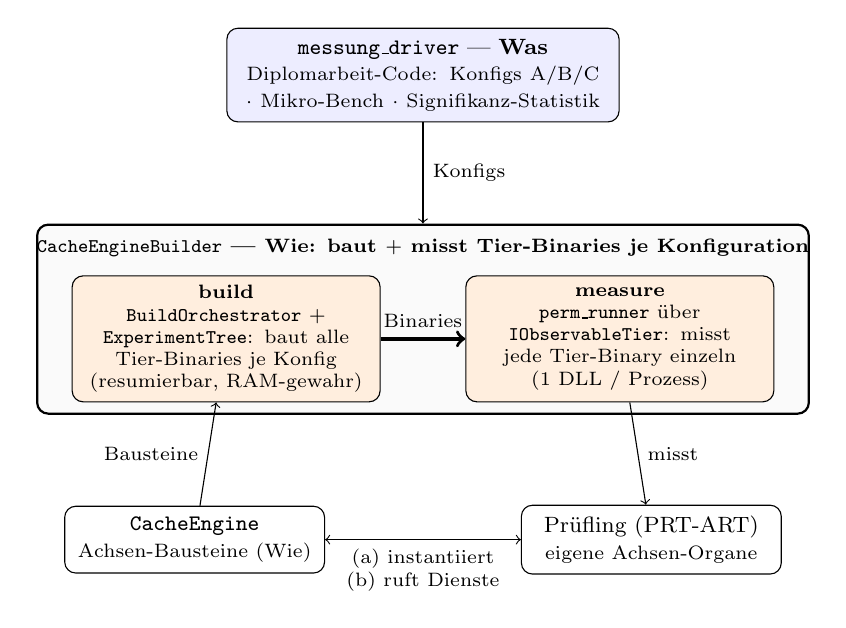
\begin{tikzpicture}[comp/.style={draw, rounded corners, align=center, font=\footnotesize, inner sep=4pt, minimum width=3.3cm},
    bm/.style={draw, rounded corners, align=center, font=\scriptsize, inner sep=3pt, text width=3.7cm, minimum height=1.6cm, fill=orange!13}]
    \node[comp,fill=blue!7,text width=4.7cm] (driver) at (0,0.6) {\texttt{messung\_driver} --- \textbf{Was}\\{\scriptsize Diplomarbeit-Code: Konfigs A/B/C $\cdot$ Mikro-Bench $\cdot$ Signifikanz-Statistik}};
    \node[draw,thick,rounded corners,minimum width=9.8cm,minimum height=2.4cm,fill=gray!4] (bbox) at (0,-2.5){};
    \node[font=\bfseries\scriptsize,anchor=north] at ([yshift=-2pt]bbox.north){\texttt{CacheEngineBuilder} --- \textbf{Wie}: baut $+$ misst Tier-Binaries je Konfiguration};
    \node[bm] (build) at (-2.5,-2.75) {\textbf{build}\\{\scriptsize \texttt{Build\-Orchestrator} $+$ \texttt{Experiment\-Tree}: baut alle Tier-Binaries je Konfig (resumierbar, RAM-gewahr)}};
    \node[bm] (measure) at (2.5,-2.75) {\textbf{measure}\\{\scriptsize \texttt{perm\_runner} über \texttt{IObservableTier}: misst jede Tier-Binary einzeln (1 DLL / Prozess)}};
    \draw[->,very thick] (build) -- node[above,font=\scriptsize]{Binaries} (measure);
    \node[comp] (engine) at (-2.9,-5.3) {\texttt{CacheEngine}\\{\scriptsize Achsen-Bausteine (Wie)}};
    \node[comp] (probe) at (2.9,-5.3) {Prüfling (PRT-ART)\\{\scriptsize eigene Achsen-Organe}};
    \draw[->] (driver) -- node[right,font=\scriptsize]{Konfigs} (bbox.north);
    \draw[->] (engine) -- node[left,font=\scriptsize]{Bausteine} (build);
    \draw[->] (measure) -- node[right,font=\scriptsize]{misst} (probe);
    \draw[<->] (engine) -- node[below, font=\scriptsize, align=center] {(a)~instantiiert\\(b)~ruft Dienste} (probe);
  \end{tikzpicture}
  \caption{Das M-Modell mit Fokus auf die Build- und Mess-Phasen. Die äußere
  \texttt{messung\_\-driver}-Schleife (\emph{Was}, Diplomarbeit-Code) speist die Konfigurationen der drei
  Messreihen A/B/C ein; der \texttt{CacheEngineBuilder} (\emph{Wie}, Bibliothek) zerfällt in die beiden
  eigentlich interessanten Phasen: \textbf{build} (\texttt{BuildOrchestrator}/\texttt{ExperimentTree} baut
  je Konfiguration eine eigenständige Tier-Binary, resumierbar und RAM-gewahr) und \textbf{measure}
  (\texttt{perm\_runner} treibt und misst jede Tier-Binary einzeln über die Beobachter-Schnittstelle
  \texttt{IObservableTier}). Die
  \texttt{CacheEngine} liefert die Standard-Achsen-Bausteine, der Prüfling PRT-ART seine eigenen Organe;
  ihre bidirektionale Beziehung ((a)~instantiiert, (b)~ruft Dienste) begründet die Multi-Prüfling-Fähigkeit. Die
  \texttt{ExecutionEngine} bleibt die gemeinsame messbare Wurzel.}\label{fig:m-model}
\end{figure}

Der Builder orchestriert eine \emph{Drei-Stufen-Prüfung}: \textbf{Stufe~1} (nur Cache-Engine) nutzt die
Standard-Variante je Achse, \textbf{Stufe~2} (nur Prüfling) ersetzt die überschriebenen Achsen durch die
Prüfling-Varianten und behält sonst die Standards, und \textbf{Stufe~3} (Full Join, nicht-redundant)
kombiniert Standard- und alle Prüfling-Varianten; im Code sind es die Verbund-Strategien des Merge-Plans
--- Stufe~1 ist \texttt{Verbund1\_CeOnly}, Stufe~2 zerfällt in Ersetzen (\texttt{Verbund2\_Replace}) und
Hybrid-Mischung (\texttt{Verbund2\_Hybrid}), Stufe~3 ist \texttt{Verbund3\_Union} ---, die die
Drei-Stufen-Sicht zusammenfasst. Jede Stufe kann bis zu tausende nicht-redundante
Permutations-Binaries erzeugen, die zur Laufzeit über die C-stabile Modulgrenze als C++23-Module geladen
werden; materialisiert wird stets eine spärliche, gedeckelte Teilmenge, der volle Produktraum wird nur
gezählt (Abbildung~\ref{fig:three-stage}).

\begin{figure}[!htbp]
  \centering
  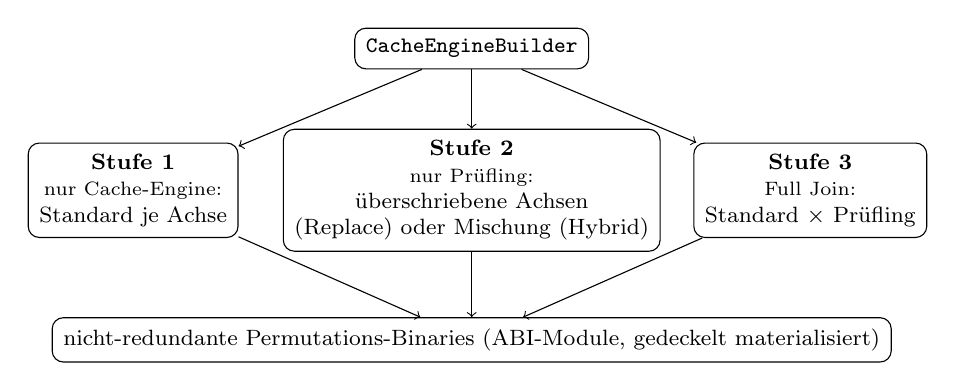
\begin{tikzpicture}[stage/.style={draw, rounded corners, align=center, font=\footnotesize, inner sep=4pt}]
    \node[draw, rounded corners, font=\footnotesize, inner sep=4pt] (b) at (0,0) {\texttt{CacheEngineBuilder}};
    \node[stage] (s1) at (-4.3,-1.8) {\textbf{Stufe~1}\\\scriptsize nur Cache-Engine:\\Standard je Achse};
    \node[stage] (s2) at (0,-1.8) {\textbf{Stufe~2}\\\scriptsize nur Prüfling:\\überschriebene Achsen\\(Replace) oder Mischung (Hybrid)};
    \node[stage] (s3) at (4.3,-1.8) {\textbf{Stufe~3}\\\scriptsize Full Join:\\Standard $\times$ Prüfling};
    \node[draw, rounded corners, align=center, font=\footnotesize, inner sep=4pt] (out) at (0,-3.7) {nicht-redundante Permutations-Binaries (ABI-Module, gedeckelt materialisiert)};
    \draw[->] (b) -- (s1);
    \draw[->] (b) -- (s2);
    \draw[->] (b) -- (s3);
    \draw[->] (s1) -- (out);
    \draw[->] (s2) -- (out);
    \draw[->] (s3) -- (out);
  \end{tikzpicture}
  \caption{Die Drei-Stufen-Prüfung des Builders: jede Stufe erzeugt nicht-redundante
  Permutations-Binaries; ihre Zuordnung zu den Messreihen~A/B/C zeigt
  Tabelle~\ref{tab:stage-series}.}\label{fig:three-stage}
\end{figure}

Diese Stufen bilden \emph{nicht} eins-zu-eins auf die drei Pflicht-Messreihen ab, sondern speisen sie: Die
Standard-Binaries der Stufe~1 (samt der rekonstruierten SOTA-Profile) und die Prüfling-Binaries der
Stufe~2 bilden \emph{gemeinsam} die Vergleichs-Messreihe~A\@; der nicht-redundante Full Join der Stufe~3 ist
die Grundlage der Variations-Messreihe~B\@; und die Merge-/Regressions-Messreihe~C (alt gegen neu) ist an
keine einzelne Stufe gebunden, sondern läuft build-übergreifend als alt-gegen-neu-Vergleich --- über
aufeinanderfolgende Stände derselben Konfiguration ebenso wie über konkrete Merge-Punkte
(Tabelle~\ref{tab:stage-series}).

\begin{table}[!htbp]
  \centering
  \caption{Zuordnung der Drei-Stufen-Prüfung zu den Pflicht-Messreihen}\label{tab:stage-series}
  \begin{tabular}{@{}lll@{}}
    \toprule
    \textbf{Prüf-Stufe} & \textbf{Inhalt} & \textbf{speist Messreihe} \\
    \midrule
    Stufe~1 (nur Cache-Engine) & Standard-Bausteine + SOTA-Profile & A (Baseline auch für C) \\
    Stufe~2 (nur Prüfling) & überschriebene Achsen = Prüfling-Varianten & A \\
    Stufe~3 (Full Join) & Standard $\times$ Prüfling, nicht-redundant & B \\
    build-übergreifend & alt gegen neu (Regression und Merge-Punkte) & C \\
    \bottomrule
  \end{tabular}

  \smallskip
  {\footnotesize Die drei Prüf-Stufen bilden nicht eins-zu-eins, sondern in dieser Zuordnung auf die
  drei Pflicht-Messreihen~A/B/C ab; Reihe~C ist build-/versionsübergreifend (nicht an eine einzelne
  Prüfstufe gebunden).\par}
\end{table}

Die drei Messreihen --- alle vom \texttt{messung\_driver} über die \texttt{ExperimentDriver}-Bibliothek
ausgeführt, konfiguriert entweder als drei feste Reihen oder über eine externe
\texttt{messreihen.xml} --- sind damit: \emph{Reihe~A} (PRT-ART vs.\ Stand der Technik) mit den Modi A\_defined
(schnelle Verifikation gegen die 8 Rang-1-Vollprofile) und A\_full (alle 33 Profile, 30 Vollprofile und 3 abstrakte; der Standard, da erst der
Voll-Lauf die bias-reduzierte Vermessung aller Lastprofile gegen alle Verfahren einlöst,
Abschnitt~\ref{sec:task-concerns}); \emph{Reihe~B} (systematische Variation der
Achsen-Entscheidungen unter sonst gleichen Bedingungen, um den Beitrag jeder Achse zu isolieren); und
\emph{Reihe~C} (Merge/Regression alt gegen neu: konkrete Merge-Punkte zwischen PRT-ART-Bausteinen und
Cache-Engine-Permutationen --- etwa das PRT-ART-OLC mit tcmalloc und ART-Page, der 4+1+2-Pool mit der
HOT-Page, das Path-Prefetch mit der B\textsuperscript{2}-Baum-Page oder das MultiLevel-Layout mit der
Wormhole-Page ---, build-übergreifend als alt-gegen-neu-Vergleich gefahren). Jede Reihe wird in
drei Granularitäten erhoben, die den drei Mess-Ebenen entsprechen
(Abschnitt~\ref{sec:measurement-system}).\ \emph{Mikro-Benchmarking} (Ebene micro) vermisst jede Achse
über ihr \emph{Achsen-Interface} --- die Funktionsmenge, die \emph{alle} Algorithmen dieser Achse liefern
müssen (jeder Allokator stellt Speicher bereit, gleich welcher): die achsen-spezifischen
Haupteigenschaften, intern gemessen. Die Achse ist dabei \emph{keine} Interface-Funktion des
Suchalgorithmus; dessen Gattungs-Interface-Funktionen \emph{verwenden} die Achsen-Interfaces ---
wie auch Achsen-Algorithmen fremde Achsen-Interfaces verwenden dürfen, denn Container etwa werden
überall gebraucht.\ \emph{Makro-Benchmarking} (Ebene macro) misst die einzelnen
\texttt{std::map}-Interface-Operationen (Einfügen, Punkt- und Bereichssuche, Aktualisieren,
Löschen) gegen Beispiel-Lasten, und \emph{Gesamt-Benchmarking} (Ebene wallclock, im CacheEngineBuilder
über die Last-Rahmenwerke) fährt die YCSB-Lastprofile über jede Rekombination --- w/ma/mi, in dieser
Reihenfolge. Als Gegenprobe zur internen Mikro-Messung misst der Apparat zusätzlich drei
\emph{Wallclock-Ebenen}: die Wallclock der Achsen-Interfaces unter jedem Algorithmus, die
Wallclock der Gattungs-Interface-Funktionen und die Wallclock einer Test-Last aus den
Last-Rahmenwerken. Architektur-Auflage dieses Schnitts ist, dass alle Achsen-Algorithmen
ausschließlich Achsen-Interfaces statt generischer Betriebssystem-Aufrufe verwenden --- inline
einkompiliert per Metaprogrammierung, ohne \texttt{std::variant} ---, damit die Mikro-Messung
einer Achse tatsächlich die Achse misst. Genau diese Methodik ist die Antwort auf das
Trennbarkeits-Problem: Indem jeder Bestandteil zunächst isoliert über sein Achsen-Interface
vermessen wird, bevor er im Operations- und Gesamt-Kontext erscheint, werden die Beiträge getrennt
messbar, statt im Gesamtdurchsatz vermengt zu bleiben.

%% INTERN-272: KA-045
Den so aufgespannten Raum reduziert das System gezielt. Der golden-Referenzkatalog --- je Organ-Achse
zwei aktivierte Vertreter, die Persistenz-Achse auf ihren In-Memory-Vertreter festgelegt --- zählt
$2^{17} = 131072$ Binary-Identitäten je System-Permutation (je Kombination der Bau-Steuergrößen,
Abschnitt~\ref{sec:axis-triad}), jede mit vollem Achtzehn-Segment-Pfad
(Abschnitt~\ref{sec:stamp-model}), und dient als Regressions-Detektor des Ganzsystems mit einer
festgeschriebenen CRC-64-Prüfsumme über alle Identitäten; die Mächtigkeit des realen Permutationsraums über alle
Achsen-Kataloge samt ihrer Unter-Achsen rechnet der Planer dagegen dynamisch aus seinen Eingängen
(Subkommando \texttt{simulate}) --- sie liegt Größenordnungen darüber und ist nie eine feste
Anzahl. Drei Mechanismen dämpfen die Explosion: Der \texttt{<expected\_workload>}-Profil-Filter routet
nur kompatible Workloads; der \texttt{Defined}-Modus führt nur die deklarierten Tupel aus, aus denen
die Messreihen des Manuskripts gespeist werden; und der \texttt{Full}- bzw.\ \texttt{Full-Sampled}-Modus
fährt den Vollraum oder eine deterministische, seed-stabile 1:$n$-Teilmenge davon (Vorgabe $n = 1000$).
Der Default-Workload ist die Voll-Permutation über alle verfügbaren Workloads; das Routing dieser
Vorgabe ist vorgesehen, aber nicht implementiert (Abschnitt~\ref{sec:eval-workloads}). Voll- und Sampled-Läufe fahren auf den registrierten
Maschinen-Signaturen --- prod1 (AMD Zen~5), prod2 (Intel Core i9-12900K, Alder Lake) und ein
ODROID-Board mit Intel-Gracemont-Kernen --- unter Beachtung der vom Plattform-Probe gemeldeten
Achsen-Kompatibilität; die Zugehörigkeit zum ZIH-Cluster der TU Dresden ist als Unter-Achse der
Ziel-ISA deklariert, ein Lauf dort ist nicht gemessen (n/a).
\end{nurlang}
\begin{nurkurz}
\subsection{Subsysteme und die Kette von der XML zur Tier-Binary}\label{sec:mess-chain}
Organisiert ist der Apparat als \emph{ein} Hauptkanal: \emph{Eine} Anwender-XML ist die einzige Quelle des
gesamten Prozesses. Sie \emph{zeigt an}, welche Experimente, Achsen, Einstellungen und Abläufe durchzuführen
sind, während je Realm ein \emph{Registry}-Katalog das \emph{Angebot} des Existierenden hält --- das deklarative
Konfigurationsmodell aus Abschnitt~\ref{sec:software-means} nach dem Vorbild des Java-POM\@; eine
unregistrierte Referenz ist ein harter Validierungsfehler. Der Experiment-\emph{Planer} löst die XML gegen die
drei Angebots-Kataloge auf und baut je Ziel-Plattform und Mess-Aufgabe \emph{einen} \texttt{CacheEngineBuilder}
(CEB), in den die gewählten Mess-Achsen einkompiliert werden; dieser orchestriert den Bau der Tier-Binaries und
stempelt sie mit seiner Plattform (Abschnitt~\ref{sec:stamp-model}); die Tier-Binary enthält die
Organ-Permutation. Jede Stufe speist sich aus ihrem art-eigenen Angebot (Mess-Katalog $\to$ Planer,
System-Katalog $\to$ Builder, Organ-Katalog $\to$ Tier-Binary), und die Tier-Binary bleibt in zwei strikt
getrennten Schichten lesbar: dem Hardware- und Umgebungs-Layer der System-Achsen und dem Anwendungs-Logik-Layer
der Organ-Achsen. Gesteuert wird die Anlage per Planer-Shell (implementiert) oder per API-Kommandozeile mit
einem headless Server; ein optionaler Erstellungsmodus deklariert die verfügbaren XML-Einstellungen aus der
erkannten Hardware; headless Dienst und Erstellungsmodus sind nicht implementiert.

Auf dieser Kette aufbauend trennt das Mess-System vier formal getrennte Subsysteme: den
\texttt{messung\_driver} (der Auswertungs-Orchestrator, der je Pflicht-Messreihe A/B/C die Pipeline durchläuft),
den \texttt{CacheEngineBuilder} (ein autonomes Plattform-Ausmess-System mit der Sieben-Phasen-Pipeline aus
Abschnitt~\ref{sec:impl-pipeline}), die \texttt{CacheEngine} (die Achsen-Bausteine-Bibliothek) und den
\texttt{Prüfling} PRT-ART (der einige Organe selbst stellt und die übrigen Cache-Engine-Dienste konsumiert);
Cache-Engine, Prüfling und diese Arbeit liegen in je eigenen Repositories, die Planer-Rolle ist als eigene
Binary realisiert (\texttt{comdare-experiment-planner}), die Builder-Rolle als Mess-Treiber
(\texttt{comdare-messung-driver}). Die \texttt{ExecutionEngine} ist kein fünftes Subsystem, sondern die
gemeinsame messbare Wurzel (\texttt{IExecutionEngine}), unter der sich Prüfling und Engines registrieren.
Definierend ist die \emph{bidirektionale} Cache-Engine\,$\leftrightarrow$\,Prüfling-Beziehung: Die Cache-Engine
instantiiert den Prüfling je Permutations-Konfiguration, und der Prüfling ruft zur Laufzeit
Cache-Engine-Dienste auf; diese Symmetrie begründet die \emph{Multi-Prüfling}-Fähigkeit, mit der Messreihe~A
den Prüfling gegen viele SOTA-Adapter in einer Pipeline vergleicht.

Der Builder orchestriert eine \emph{Drei-Stufen-Prüfung}: \textbf{Stufe~1} (nur Cache-Engine) nutzt die
Standard-Variante je Achse, \textbf{Stufe~2} (nur Prüfling) ersetzt die überschriebenen Achsen durch die
Prüfling-Varianten, und \textbf{Stufe~3} (Full Join, nicht-redundant) kombiniert Standard- und alle
Prüfling-Varianten; im Code sind es die Verbund-Strategien des Merge-Plans --- Stufe~1 ist
\texttt{Verbund1\_CeOnly}, Stufe~2 zerfällt in Ersetzen (\texttt{Verbund2\_Replace}) und Hybrid-Mischung
(\texttt{Verbund2\_Hybrid}), Stufe~3 ist \texttt{Verbund3\_Union}. Jede Stufe kann tausende nicht-redundante
Permutations-Binaries erzeugen, die zur Laufzeit über die C-stabile Modulgrenze als C++23-Module geladen
werden; materialisiert wird stets eine gedeckelte Teilmenge, der volle Produktraum nur gezählt.

Diese Stufen bilden \emph{nicht} eins-zu-eins auf die drei Pflicht-Messreihen ab, sondern speisen sie: Die
Standard-Binaries der Stufe~1 (samt der rekonstruierten SOTA-Profile) und die Prüfling-Binaries der
Stufe~2 bilden \emph{gemeinsam} die Vergleichs-Messreihe~A\@; der nicht-redundante Full Join der Stufe~3 ist
die Grundlage der Variations-Messreihe~B\@; und die Merge-/Regressions-Messreihe~C (alt gegen neu) ist an
keine einzelne Stufe gebunden, sondern läuft build-übergreifend als alt-gegen-neu-Vergleich --- über
aufeinanderfolgende Stände derselben Konfiguration ebenso wie über konkrete Merge-Punkte
(Tabelle~\ref{tab:stage-series}).

\begin{table}[!htbp]
  \centering
  \caption{Zuordnung der Drei-Stufen-Prüfung zu den Pflicht-Messreihen}\label{tab:stage-series}
  \begin{tabular}{@{}lll@{}}
    \toprule
    \textbf{Prüf-Stufe} & \textbf{Inhalt} & \textbf{speist Messreihe} \\
    \midrule
    Stufe~1 (nur Cache-Engine) & Standard-Bausteine + SOTA-Profile & A (Baseline auch für C) \\
    Stufe~2 (nur Prüfling) & überschriebene Achsen = Prüfling-Varianten & A \\
    Stufe~3 (Full Join) & Standard $\times$ Prüfling, nicht-redundant & B \\
    build-übergreifend & alt gegen neu (Regression und Merge-Punkte) & C \\
    \bottomrule
  \end{tabular}

  \smallskip
  {\footnotesize Die drei Prüf-Stufen bilden nicht eins-zu-eins, sondern in dieser Zuordnung auf die
  drei Pflicht-Messreihen~A/B/C ab; Reihe~C ist build-/versionsübergreifend (nicht an eine einzelne
  Prüfstufe gebunden).\par}
\end{table}

Die drei Messreihen sind damit: \emph{Reihe~A} (PRT-ART vs.\ Stand der Technik) mit den Modi A\_defined
(schnelle Verifikation gegen die 8 Rang-1-Vollprofile) und A\_full (alle 33 Profile; der Standard, da erst der
Voll-Lauf die bias-reduzierte Vermessung aller Lastprofile gegen alle Verfahren einlöst,
Abschnitt~\ref{sec:task-concerns}); \emph{Reihe~B} (Variation der Achsen-Entscheidungen unter sonst gleichen
Bedingungen, um den Beitrag jeder Achse zu isolieren); und \emph{Reihe~C} (Merge/Regression alt gegen neu über
konkrete Merge-Punkte, build-übergreifend gefahren). Jede Reihe wird in drei Granularitäten erhoben, die den
drei Mess-Ebenen entsprechen (Abschnitt~\ref{sec:measurement-system}): \emph{Mikro-Benchmarking} (micro)
vermisst jede Achse über ihr \emph{Achsen-Interface} --- die Funktionsmenge, die \emph{alle} Algorithmen dieser
Achse liefern müssen ---, \emph{Makro-Benchmarking} (macro) die einzelnen \texttt{std::map}-Interface-Operationen
gegen Beispiel-Lasten und \emph{Gesamt-Benchmarking} (wallclock, über die Last-Rahmenwerke) die YCSB-Lastprofile
über jede Rekombination --- w/ma/mi, in dieser Reihenfolge; als Gegenprobe misst der Apparat zusätzlich drei
Wallclock-Ebenen (Achsen-Interfaces, Gattungs-Interface-Funktionen, Test-Last aus den Last-Rahmenwerken).
Architektur-Auflage dieses Schnitts: alle Achsen-Algorithmen verwenden ausschließlich Achsen-Interfaces statt
generischer Betriebssystem-Aufrufe --- inline einkompiliert, ohne \texttt{std::variant} ---, damit die
Mikro-Messung einer Achse tatsächlich die Achse misst. Genau diese Methodik ist die Antwort auf das
Trennbarkeits-Problem: Jeder Bestandteil wird zunächst isoliert über sein Achsen-Interface vermessen, bevor er
im Operations- und Gesamt-Kontext erscheint; die Beiträge bleiben getrennt messbar, statt im Gesamtdurchsatz
vermengt zu bleiben.

Den so aufgespannten Raum reduziert das System gezielt. Der golden-Referenzkatalog --- je Organ-Achse zwei
aktivierte Vertreter, die Persistenz-Achse auf ihren In-Memory-Vertreter festgelegt --- zählt $2^{17} = 131072$
Binary-Identitäten je System-Permutation (Abschnitt~\ref{sec:axis-triad}), jede mit vollem
Achtzehn-Segment-Pfad (Abschnitt~\ref{sec:stamp-model}), und dient als Regressions-Detektor mit einer
festgeschriebenen CRC-64-Prüfsumme; die Mächtigkeit des realen Permutationsraums rechnet der Planer dagegen
dynamisch aus seinen Eingängen (Subkommando \texttt{simulate}) --- sie liegt Größenordnungen darüber und ist nie
eine feste Anzahl. Drei Mechanismen dämpfen die Explosion: der \texttt{<expected\_workload>}-Profil-Filter (nur
kompatible Workloads), der \texttt{Defined}-Modus (nur die deklarierten Tupel) und der \texttt{Full}- bzw.\
\texttt{Full-Sampled}-Modus (Vollraum oder seed-stabile 1:$n$-Teilmenge). Der Default-Workload ist die
Voll-Permutation über alle verfügbaren Workloads; das Routing dieser Vorgabe ist nicht implementiert
(Abschnitt~\ref{sec:eval-workloads}). Voll- und Sampled-Läufe fahren auf den registrierten Maschinen-Signaturen
prod1 (AMD Zen~5), prod2 (Intel Core i9\mbox{-}12900K, Alder Lake) und einem ODROID-Board mit
Intel-Gracemont-Kernen; ein Lauf auf dem ZIH-Cluster der TU Dresden ist nicht gemessen (n/a).
\end{nurkurz}

\begin{nurlang}
\section{PRT-ART als Demonstrator}\label{sec:prtart-demo}
PRT-ART ist der \emph{Prüfling}, an dem sich die Tragfähigkeit des Systems zeigt: ein abstraktes Lebewesen, das einige
Achsen-Organe selbst stellt und die übrigen über die Verbund-Strategie des Merge-Plans aus dem
Standard-Baukasten der Cache-Engine bezieht (Abschnitt~\ref{sec:mess-chain}) --- als monomorphe
CRTP-Concept-Achsen, ohne Laufzeit-Fallback; die hybride
\texttt{PrtArtSearchEngine<Ts\ldots>}-API bleibt davon unberührt, und die Laufzeit-Anbindung erfolgt über
den Execution-Engine-Adapter, nicht über eine eigene Such-Engine-Schicht. Geladen wird das
Prüfling-Repo über den Plugin-Controller der Cache-Engine
(\texttt{COMDARE\_\allowbreak{}CE\_\allowbreak{}PRUEFLINGE}): Sein Einstiegs-Snippet muss sich per
\texttt{comdare\_\allowbreak{}pruefling\_\allowbreak{}deklarieren} ausdrücklich \emph{zusichern} ---
mit der einzigen registrierten Fähigkeit
\texttt{pruefling\_\allowbreak{}slots\_\allowbreak{}v1}, den Prüflings-Slots ---, denn
Anwesenheit darf nur widerlegen, nie erlauben: Die hinterlegten Beleg-Header können die Zusicherung
nur brechen, niemals ein Gatter öffnen, und ein angeforderter, aber nicht deklarierender Prüfling
bricht die Konfiguration mit Fehlermeldung ab, statt still übersprungen zu werden; ein prüfling-eigener
Adapter-Pfad ist deaktiviert und nicht Teil dieser Zusicherung.
Was PRT-ART beiträgt, liegt auf drei Ebenen. Erstens die \emph{Prüflings-Slots} im eigenen Repository:
die Build-Achse Page-Type, der Prefetch, das Wert-Handle (ChainRef) und das Telemetrie-Tooling mit den
Hypothesen-Metriken H1/H2/H3 (in der Dreiteilung eine Mess-Tooling-Unter-Achse,
Abschnitt~\ref{sec:axis-triad}); die Bewertung der Hypothesen-Metriken enthalten die
Kapitel~\ref{ch:eval} und~\ref{ch:conclusion}. Zweitens die Referenz-Komposition der Cache-Engine,
\texttt{PrtArtComposition}, die sich von der ART-Komposition in genau einer Achse unterscheidet --- der
Pfadkompression als Redirect-Organ, dem \emph{R} in PRT-ART\@; das optimistische Lock-Coupling ist von
ART geerbt, kein PRT-ART-Beitrag. Drittens die codegen-fähige Prüflings-Komposition, die sechzehn von
achtzehn Achsen aus der ART-Komposition übernimmt und Prefetch sowie Wert-Handle durch die
Prüflings-Slots ersetzt. Seine weiteren eigenen Bausteine, der 4+1+2-Pool-Allokator
(Free-List-Unter-Achse) und das MultiLevel-Layout, liegen im Prüfling-Repo und laufen im Mess-Pfad über
den Cache-Engine-Standard (Anbindung als nachfolgender Umsetzungsschritt vorgesehen, aber nicht
implementiert); für die übrigen Achsen verwendet er bestehende
SOTA-Bausteine über die Permutations-Konfiguration wieder. So belegt der Prüfling, dass das Mess-System
tragfähig ist: Ein neuartiges Lebewesen entsteht aus wenigen eigenen Organen plus dem Standard-Baukasten
(Abbildung~\ref{fig:prtart-demo}) und ist über dasselbe Prüf-Dock messbar wie jedes rekonstruierte
SOTA-Verfahren.

%% INTERN-272: KA-046
\begin{figure}[htbp]\centering
%% INTERN-272: KA-047
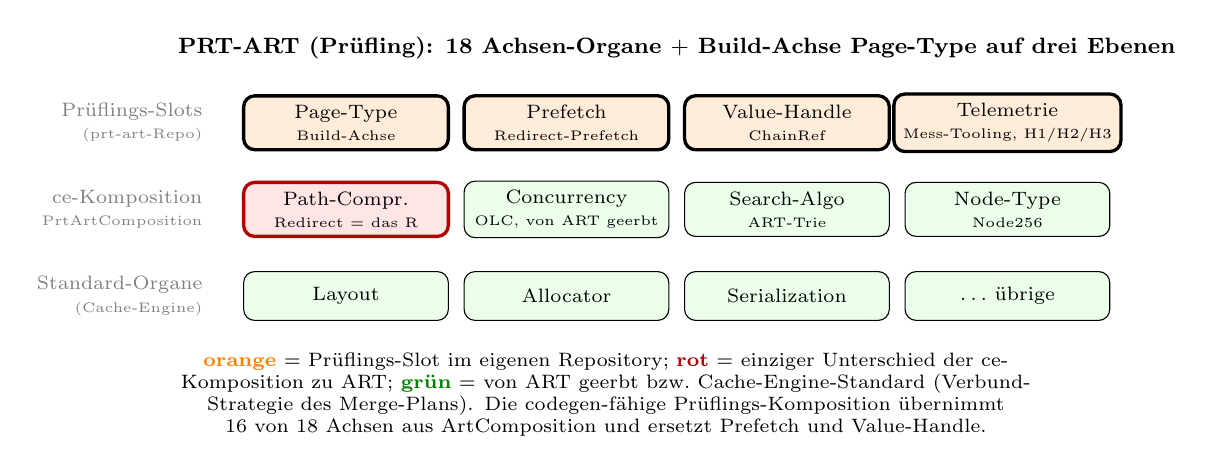
\begin{tikzpicture}[font=\footnotesize,align=center,
  prt/.style={draw,rounded corners,fill=orange!15,very thick,minimum width=2.6cm,minimum height=0.62cm,font=\scriptsize},
  ce/.style={draw,rounded corners,fill=green!8,minimum width=2.6cm,minimum height=0.62cm,font=\scriptsize},
  rd/.style={draw,rounded corners,fill=red!10,very thick,draw=red!70!black,minimum width=2.6cm,minimum height=0.62cm,font=\scriptsize},
  row/.style={font=\scriptsize,anchor=east,text=gray,align=right}]
  \node[font=\bfseries\footnotesize] at (2.9,2.55){PRT-ART (Prüfling): 18 Achsen-Organe $+$ Build-Achse Page-Type auf drei Ebenen};
  \node[row] at (-3.0,1.6){Prüflings-Slots\\{\tiny (prt-art-Repo)}};
  \node[prt] at (-1.3,1.6){Page-Type\\{\tiny Build-Achse}};
  \node[prt] at (1.5,1.6){Prefetch\\{\tiny Redirect-Prefetch}};
  \node[prt] at (4.3,1.6){Value-Handle\\{\tiny ChainRef}};
  \node[prt] at (7.1,1.6){Telemetrie\\{\tiny Mess-Tooling, H1/H2/H3}};
  \node[row] at (-3.0,0.5){ce-Komposition\\{\tiny PrtArtComposition}};
  \node[rd] at (-1.3,0.5){Path-Compr.\\{\tiny Redirect $=$ das R}};
  \node[ce] at (1.5,0.5){Concurrency\\{\tiny OLC, von ART geerbt}};
  \node[ce] at (4.3,0.5){Search-Algo\\{\tiny ART-Trie}};
  \node[ce] at (7.1,0.5){Node-Type\\{\tiny Node256}};
  \node[row] at (-3.0,-0.6){Standard-Organe\\{\tiny (Cache-Engine)}};
  \node[ce] at (-1.3,-0.6){Layout};
  \node[ce] at (1.5,-0.6){Allocator};
  \node[ce] at (4.3,-0.6){Serialization};
  \node[ce] at (7.1,-0.6){$\ldots$ übrige};
  \node[font=\scriptsize,align=center,text width=13.2cm] at (2.0,-1.85){\textcolor{orange}{\textbf{orange}} $=$ Prüflings-Slot im eigenen Repository; \textcolor{red!70!black}{\textbf{rot}} $=$ einziger Unterschied der ce-Komposition zu ART; \textcolor{green!50!black}{\textbf{grün}} $=$ von ART geerbt bzw.\ Cache-Engine-Standard (Verbund-Strategie des Merge-Plans). Die codegen-fähige Prüflings-Komposition übernimmt 16 von 18 Achsen aus ArtComposition und ersetzt Prefetch und Value-Handle.};
\end{tikzpicture}
\caption{PRT-ART als Demonstrator im M-Modell auf drei Ebenen: die vier Prüflings-Slots im eigenen Repository (Page-Type als Build-Achse, Prefetch, Wert-Handle, Telemetrie als Mess-Tooling-Unter-Achse, Abschnitt~\ref{sec:axis-triad}); die Referenz-Komposition der Cache-Engine, die sich von ART in genau einer Achse --- der Pfadkompression als Redirect-Organ --- unterscheidet, während das optimistische Lock-Coupling von ART geerbt ist; und die codegen-fähige Prüflings-Komposition, die sechzehn von achtzehn Achsen aus der ART-Komposition übernimmt und Prefetch sowie Wert-Handle ersetzt. Die weiteren eigenen Bausteine (4+1+2-Pool-Allokator, MultiLevel-Layout) laufen im Mess-Pfad über den Cache-Engine-Standard (Anbindung: nachfolgender Umsetzungsschritt, nicht implementiert). So entsteht ein vollständiges, mess-fähiges Lebewesen aus wenigen eigenen plus vielen Standard-Organen.}\label{fig:prtart-demo}
\end{figure}
\end{nurlang}
\begin{nurkurz}
\section{PRT-ART als Demonstrator}\label{sec:prtart-demo}
PRT-ART ist der \emph{Prüfling}, an dem sich die Tragfähigkeit des Systems zeigt: ein abstraktes Lebewesen, das
einige Achsen-Organe selbst stellt und die übrigen über die Verbund-Strategie des Merge-Plans aus dem
Standard-Baukasten der Cache-Engine bezieht (Abschnitt~\ref{sec:mess-chain}) --- als monomorphe
CRTP-Concept-Achsen, ohne Laufzeit-Fallback; die Laufzeit-Anbindung erfolgt über den Execution-Engine-Adapter.
Geladen wird das Prüfling-Repo über den Plugin-Controller der Cache-Engine: Sein Einstiegs-Snippet muss sich
per \texttt{comdare\_\allowbreak{}pruefling\_\allowbreak{}deklarieren} ausdrücklich \emph{zusichern} (einzige
registrierte Fähigkeit: die Prüflings-Slots), denn Anwesenheit darf nur widerlegen, nie erlauben; ein
angeforderter, aber nicht deklarierender Prüfling bricht die Konfiguration mit Fehlermeldung ab. Was PRT-ART
beiträgt, liegt auf drei Ebenen. Erstens die \emph{Prüflings-Slots} im eigenen Repository: die Build-Achse
Page-Type, der Prefetch, das Wert-Handle (ChainRef) und das Telemetrie-Tooling mit den Hypothesen-Metriken
H1/H2/H3 (eine Mess-Tooling-Unter-Achse, Abschnitt~\ref{sec:axis-triad}); ihre Bewertung enthalten die
Kapitel~\ref{ch:eval} und~\ref{ch:conclusion}. Zweitens die Referenz-Komposition der Cache-Engine,
\texttt{PrtArtComposition}, die sich von der ART-Komposition in genau einer Achse unterscheidet --- der
Pfadkompression als Redirect-Organ, dem \emph{R} in PRT-ART\@; das optimistische Lock-Coupling ist von ART
geerbt. Drittens die codegen-fähige Prüflings-Komposition, die sechzehn von achtzehn Achsen aus der
ART-Komposition übernimmt und Prefetch sowie Wert-Handle durch die Prüflings-Slots ersetzt. Seine weiteren
eigenen Bausteine, der 4+1+2-Pool-Allokator und das MultiLevel-Layout, laufen im Mess-Pfad über den
Cache-Engine-Standard (Anbindung vorgesehen, nicht implementiert). So belegt der Prüfling, dass das Mess-System
tragfähig ist: Ein neuartiges Lebewesen entsteht aus wenigen eigenen Organen plus dem Standard-Baukasten und
ist über dasselbe Prüf-Dock messbar wie jedes rekonstruierte SOTA-Verfahren.
\end{nurkurz}

\section{Schärfung durch Heuristiken}\label{sec:heuristics}
Die Messreihen liefern mehr als Ranglisten: Aus ihnen lassen sich Heuristiken gewinnen, die das
Mess-System schrittweise von einem Prüfstand zu einem sich selbst optimierenden Auslieferungs-System
schärfen. Dieser Abschnitt entwickelt diese Schärfung als Konzept in drei Stufen --- die
Heuristik-Schleife über gelernte Lastprofile, die vier Betriebsmodi des Builders bis zum Hybrid-Modus
als Zielbild der Arbeit und das Messkurven-Typsystem samt Filterkette und Messfehler-Erkennung, das
diese Modi mit Daten versorgt.

\begin{nurlang}
\subsection{Heuristik-Schleife und gelernte Lastprofile}\label{sec:heuristics-loop}
Aus den Messreihen lässt sich je Last- und Datentyp-Profil die beste
Achsen-Komposition ableiten und als wiederverwendbares Profil ablegen.
\begin{figure}[htbp]\centering
\begin{tikzpicture}[font=\footnotesize,>=Stealth,thick,align=center,
  stage/.style={draw,rounded corners,fill=blue!4,minimum width=2.8cm,minimum height=1cm}]
  \node[stage] (mess) at (0,0){Messung\\{\scriptsize Messreihen A/B/C}};
  \node[stage] (profil) at (4.4,0){XML-Lastprofil\\{\scriptsize gelernte Zuordnung}};
  \node[stage] (konfig) at (4.4,-2.2){Konfiguration\\{\scriptsize beste Achsen-Komposition}};
  \node[stage] (filter) at (0,-2.2){Workload-Filter\\{\scriptsize \texttt{<expected\_workload>}}};
  \draw[->] (mess)--(profil);\draw[->] (profil)--(konfig);
  \draw[->] (konfig)--(filter);\draw[->] (filter)--(mess);
\end{tikzpicture}
\caption{Die Heuristik-Schleife: aus den Messreihen wird je Lastprofil die beste Achsen-Komposition gelernt, als XML-Lastprofil abgelegt und über den Workload-Filter in die nächste Messung zurückgeführt.}\label{fig:heuristic-loop}
\end{figure}

%% INTERN-272: KA-048
\emph{Die volle Schleife ist ein Ausblick-Mechanismus; realisiert sind davon die automatische Auswahl
und der Binary-Versand (Abschnitt~\ref{sec:contributions}).} Der Selektor liest die Messwert-Mappe ---
die xlsx-Mappe ist die Ausgabe und der Standard des Apparats; die CSV-Form ist kein einzelnes
Kind-Dokument, sondern ein aus der Mappe erzeugter, geordneter Baum aus CSV-Dateien mit denselben Spalten
(ein Gesamtordner je Mappe, darunter ein Ordner je Blatt, darin die CSV-Dateien der einzelnen
Unter-Achsen-Fahrten) ---, rankt je
Interface-Funktion und Metrik über die gültigen Zwei-Phasen-Zeilen (Median, Nearest-Rank), bestimmt bei
konkurrierenden Zielgrößen die Pareto-Front der nicht-dominierten Kandidaten statt eines Einzelsiegers,
löst die \texttt{binary\_id} zur Binary im Lager auf und liefert Binary, Versions-Sidecar und Manifest
als eigenständiges Artefakt aus. Die Heuristik-Kurven entstehen als natürliche kubische Splines über die
Stützstellen je Achse und $x$-Dimension; ein Entscheidungs-Lambda-Baum liest die Break-Even-Schwellen
aus den Spline-Schnittpunkten und wählt an einer Anfrage-Koordinate rückwärts die führende Binary ---
synthetische Stützstellen weist er als Gerüst aus, ohne gültige Kurven trifft er keine Entscheidung.
Über die reine Rangbildung hinaus ist eine \emph{Heuristik-Extraktion} als Folge-Phase nach
\textbf{Persist} --- der letzten Phase der Sieben-Phasen-Pipeline (Abschnitt~\ref{sec:impl-pipeline}) ---
vorgesehen, die aus den gesammelten Messungen automatisch ableitet, welche Achsen-Konfiguration je Workload
und Datensatz die beste ist. Der angestrebte Mechanismus ist eine ML-Klassifikation in drei Schritten:
Zunächst werden aus der Messwert-Mappe je Permutation Merkmale gewonnen --- die Lastprofil- und Datensatz-Merkmale (Workload-Typ,
Schlüssel-Verteilung, Schreib-/Lese-Anteil, Alphabet- und Präfix-Charakteristik sowie Schlüssel- und
Wert-Datentyp) sowie die Achsen-Belegung ---, mit der je
Lastmuster gemessenen Bestleistung (etwa Durchsatz oder Tail-Latenz) als Zielgröße; darüber lernt ein \emph{ML-Klassifikator} die Abbildung
von Lastprofil-/Achsen-Merkmalen auf die beste Konfiguration; und dieser liefert je Workload-/Datensatz-Klasse
die empfohlene Achsen-Komposition, ohne den gesamten Permutationsraum erneut zu fahren. Das Ergebnis wird
als wiederverwendbares \emph{XML-Lastprofil} persistiert --- symmetrisch zu den Messreihen-XML-Konfigurationen
--- und kann ohne erneute Vollvermessung in den \texttt{<expected\_workload>}-Filter zurückgespeist werden;
damit schließt sich der Kreis zwischen Messung, gelernter Heuristik und konfigurationsleitender Auswahl
(Abbildung~\ref{fig:heuristic-loop}). Dieser \emph{measure $\to$ profile $\to$ config $\to$
filter}-Kreislauf ist die klassische, etablierte Form des \emph{empirischen, messgetriebenen Autotunings}:
Er steht in der Linie von Autotuning-Frameworks wie OpenTuner~\cite{ansel2014opentuner} und den
messen-im-Kreis-Autotunern FFTW~\cite{frigo1998fftw} und ATLAS~\cite{whaley2001atlas}; die
lastprofil-getriebene Konfigurationswahl mit Workload-Filter findet ihre Datenbank-Entsprechung in
OtterTune~\cite{vanaken2017ottertune} und im Database Tuning Advisor mit Workload-Kompression~\cite{agrawal2005autoadmin},
die online-laufzeitnahe Variante in Active Harmony~\cite{tapus2002activeharmony}; die Bezeichnung
\enquote{Software-in-the-Loop} selbst entstammt der X-in-the-Loop-Validierungstaxonomie~\cite{tibba2016xil}.
Die ML-Klassifikation ist nicht implementiert und bleibt zukünftiger Arbeit vorbehalten
(Kapitel~\ref{ch:conclusion}); die Schleife selbst ist jedoch nur die erste Stufe eines größeren
Betriebs-Zielbilds, das der folgende Unterabschnitt entwickelt.
\end{nurlang}
\begin{nurkurz}
\subsection{Heuristik-Schleife und gelernte Lastprofile}\label{sec:heuristics-loop}
Aus den Messreihen lässt sich je Last- und Datentyp-Profil die beste
Achsen-Komposition ableiten und als wiederverwendbares Profil ablegen.

\emph{Die volle Schleife ist ein Ausblick-Mechanismus; realisiert sind davon die automatische Auswahl und der
Binary-Versand (Abschnitt~\ref{sec:contributions}).} Der Selektor liest die Messwert-Mappe --- die xlsx-Mappe
ist die Ausgabe des Apparats, die CSV-Form ihr aus ihr erzeugter Baum-Abzug (Abschnitt~\ref{sec:eval-dataflow})
---, rankt je Interface-Funktion und Metrik über die gültigen Zwei-Phasen-Zeilen (Median, Nearest-Rank),
bestimmt bei konkurrierenden Zielgrößen die Pareto-Front, löst die \texttt{binary\_id} zur Binary im Lager auf
und liefert Binary, Versions-Sidecar und Manifest aus. Die Heuristik-Kurven entstehen als natürliche kubische
Splines über die Stützstellen je Achse und $x$-Dimension; ein Entscheidungs-Lambda-Baum liest die
Break-Even-Schwellen aus den Spline-Schnittpunkten und wählt an einer Anfrage-Koordinate die führende Binary.
Über die reine Rangbildung hinaus ist eine \emph{Heuristik-Extraktion} als Folge-Phase nach \textbf{Persist},
der letzten Phase der Sieben-Phasen-Pipeline (Abschnitt~\ref{sec:impl-pipeline}), als ML-Klassifikation in drei
Schritten vorgesehen: Aus der Messwert-Mappe werden je Permutation Lastprofil-, Datensatz- und Achsen-Merkmale
mit der gemessenen Bestleistung als Zielgröße gewonnen; ein \emph{ML-Klassifikator} lernt darüber die Abbildung
auf die beste Konfiguration; und er liefert je Workload-/Datensatz-Klasse die empfohlene Achsen-Komposition,
ohne den Permutationsraum erneut zu fahren. Das Ergebnis wird als wiederverwendbares \emph{XML-Lastprofil}
persistiert und in den \texttt{<expected\_workload>}-Filter zurückgespeist; dieser \emph{measure $\to$ profile
$\to$ config $\to$ filter}-Kreislauf ist messgetriebenes Autotuning in der Linie von
OpenTuner~\cite{ansel2014opentuner}, FFTW~\cite{frigo1998fftw} und ATLAS~\cite{whaley2001atlas}, mit der
Datenbank-Entsprechung in OtterTune~\cite{vanaken2017ottertune} und dem Database Tuning
Advisor~\cite{agrawal2005autoadmin}, der online-laufzeitnahen Variante in Active
Harmony~\cite{tapus2002activeharmony} und der Bezeichnung \enquote{Software-in-the-Loop} aus der
X-in-the-Loop-Taxonomie~\cite{tibba2016xil}. Die ML-Klassifikation ist nicht implementiert
(Kapitel~\ref{ch:conclusion}); die Schleife selbst ist nur die erste Stufe des Betriebs-Zielbilds, das der
folgende Unterabschnitt entwickelt.
\end{nurkurz}

\begin{nurlang}
\subsection{Die vier Betriebsmodi des Builders}\label{sec:heuristics-modes}
%% INTERN-272: KA-049
Die Heuristik-Schleife ist der Kern eines Betriebsregimes aus \emph{vier} aufeinander aufbauenden
Betriebsmodi des Builder-Interfaces. Von der Ablauf-Kette build $\to$ measure $\to$ compare $\to$ release
(Abschnitt~\ref{sec:anatomy-levels}, Abbildung~\ref{fig:modi-kette}) sind diese Betriebs-Zielbilder zu
unterscheiden, in denen der Apparat betrieben wird; die Zuordnung ist eindeutig: Der \emph{Mess-Modus}
umfasst build und measure, der \emph{Auswertungs-Modus} ist compare, der \emph{Arbeits-Modus} ist der
release einer Einzel-Binary, und der \emph{Hybrid-Modus} ist der release einer Hybrid-Rekombination,
deren Kette sich auf der Hybrid-Ebene wiederholt. Der erste Modus ist der Betrieb des Apparats; die Modi
zwei bis vier sind das erklärte Ziel dieser Arbeit und werden hier als Konzept festgehalten. Der
Hybrid-Modus ist dabei ein erweitertes, optionales Konstrukt: Der Kern der Arbeit ist das Durchmessen
und Erstellen der Tier-Binaries samt Break-Even-Analyse vor jeder Anwendung des Hybriden, und die Arbeit
geht in der Kette nicht über die Vergleichsstufe der Hybrid-Ebene (\texttt{hybrid-compare}) nach der
Auslieferungsstufe der Einzel-Binary (\texttt{single-release}) hinaus. Von diesen vier
Betriebsmodi zu unterscheiden ist der in Teilfrage FF2.c (Abschnitt~\ref{sec:rqs}) erfragte
\emph{Paper-Isolations-Modus}: ein Betriebsmodus, der die Entwurfsbestandteile genau einer
Veröffentlichung als \emph{Achsen-Set} --- die geschlossene Achsenmenge dieses einen Referenzentwurfs,
bei weiterhin freistehenden Mess- und System-Achsen --- isoliert anbietet, um die Veröffentlichung
originalgetreu durchzumessen; er ist nicht implementiert und bleibt Ausblick (Abschnitt~\ref{sec:outlook}).
\end{nurlang}
\begin{nurkurz}
\subsection{Die vier Betriebsmodi des Builders}\label{sec:heuristics-modes}
%% INTERN-272: KA-049
Die Heuristik-Schleife ist der Kern eines Betriebsregimes aus \emph{vier} aufeinander aufbauenden Betriebsmodi
des Builder-Interfaces, die von der Ablauf-Kette build $\to$ measure $\to$ compare $\to$ release
(Abschnitt~\ref{sec:anatomy-levels}, Abbildung~\ref{fig:modi-kette}) zu unterscheiden sind; die Zuordnung ist
eindeutig: Der \emph{Mess-Modus} umfasst build und measure, der \emph{Auswertungs-Modus} ist compare, der
\emph{Arbeits-Modus} der release einer Einzel-Binary und der \emph{Hybrid-Modus} der release einer
Hybrid-Rekombination, deren Kette sich auf der Hybrid-Ebene wiederholt. Der erste Modus ist der Betrieb des
Apparats; die Modi zwei bis vier sind das erklärte Ziel dieser Arbeit und werden als Konzept festgehalten ---
der Kern ist das Durchmessen und Erstellen der Tier-Binaries samt Break-Even-Analyse vor jeder Anwendung des
Hybriden, und die Arbeit geht in der Kette nicht über \texttt{hybrid-compare} nach \texttt{single-release}
hinaus. Davon zu unterscheiden ist der in Teilfrage FF2.c (Abschnitt~\ref{sec:rqs}) erfragte
\emph{Paper-Isolations-Modus}, der die Entwurfsbestandteile genau einer Veröffentlichung als geschlossenes
\emph{Achsen-Set} isoliert anbietet, um sie originalgetreu durchzumessen; er ist nicht implementiert und bleibt
Ausblick (Abschnitt~\ref{sec:outlook}).
\end{nurkurz}

\begin{nurlang}
%% INTERN-272: KA-050
Im \emph{Mess-Modus} --- dem Betrieb, den Abschnitt~\ref{sec:measurement-system} beschreibt --- fährt
der Builder die Messreihen über die zugelassenen Permutationen. Nach Abschluss der Messung kennt das
Framework die Eigenschaften aller zugelassenen Achsen-Algorithmen gegen die Rekombination aller
zugelassenen Lastprofil-Rahmenwerke und Workloads. Der \emph{Auswertungs-Modus} verdichtet diese
Messungen: Aus ihnen ergeben sich minimale Stränge der Permutationen aller Eigenschaften gegeneinander
für bestimmte \emph{Workload-Cluster} --- für Gruppen ähnlicher Lasten bleibt der kleine Satz von
Achsen-Kompositionen übrig, der sie dominiert. Workloads werden dafür nach möglichst ähnlichen Abfolgen
gleicher Zugriffsmuster auf die Gattungs- und Genus-Interfaces der Tier-Binaries geclustert: Jedes
Last-Rahmenwerk durchläuft seine geplante Strategie einmal trocken, und Abfolge, Häufigkeit und
Anforderungen seiner Interface-Aufrufe werden notiert --- das, was ein Durchlauf des Rahmenwerks statisch
von sich gibt. Daraus entsteht je Profil ein gerichteter Übergangsgraph der Interface-Zugriffe mit
absoluten und relativen Folgewahrscheinlichkeiten (die Abbildung eines Interfaces auf sich selbst ist
als Kante zugelassen); seine Kantenmatrix wird mit dem EM-Algorithmus~\cite{dempster1977em}
ausgewertet, und die Abstände der Mittelpunkte der Wahrscheinlichkeits-Punktwolken zueinander ergeben
je Profil ein \emph{Punkt-Wolken-Wort} variabler Länge (kürzer, wenn Interfaces nicht aufgerufen werden
--- null-gefiltert). Die lexikografische Sortierung dieser Wörter ist die Mess-Reihenfolge:
Nebeneinanderliegende Wörter sind ähnliche Lasten und werden --- gleich aus welchem Rahmenwerk sie
stammen --- hintereinander gefahren. Dieses Verfahren ist im Code nicht implementiert; es ist zugleich die
vierte Auswertungs-Komponente des Hybrid-Tiers (Abschnitt~\ref{sec:heuristics-curves}).
\end{nurlang}
\begin{nurkurz}
Im \emph{Mess-Modus} --- dem Betrieb, den Abschnitt~\ref{sec:measurement-system} beschreibt --- fährt der
Builder die Messreihen über die zugelassenen Permutationen; danach kennt das Framework die Eigenschaften aller
zugelassenen Achsen-Algorithmen gegen alle Lastprofil-Rahmenwerke und Workloads. Der \emph{Auswertungs-Modus}
verdichtet diese Messungen zu minimalen Strängen je \emph{Workload-Cluster}: Für Gruppen ähnlicher Lasten
bleibt der kleine Satz von Achsen-Kompositionen übrig, der sie dominiert. Geclustert werden Workloads nach
ähnlichen Abfolgen gleicher Zugriffsmuster auf die Gattungs- und Genus-Interfaces (je Profil ein gerichteter
Übergangsgraph der Interface-Zugriffe mit Folgewahrscheinlichkeiten, dessen Clusterung zugleich die
Mess-Reihenfolge festlegt). Dieses Verfahren ist nicht implementiert; es ist zugleich die vierte
Auswertungs-Komponente des Hybrid-Tiers (Abschnitt~\ref{sec:heuristics-curves}).
\end{nurkurz}

\begin{nurlang}
%% INTERN-272: KA-051
Der \emph{Arbeits-Modus} ist das Produktions-Ziel: Das Builder-Interface hält alle für die aktuell
stochastisch häufig auftretende Workload-Last und Interface-Funktion relevanten Tier-Binaries vorgeladen im
Arbeitsspeicher und wechselt intern die Tier-Binary mit ihren speziell optimalen
Achsen-Permutationen am ABI-stabilen Interface --- derselbe Mechanismus des Binary-Wechsels, den der
Mess-Modus nutzt, nur last-getrieben statt mess-getrieben. Ebenen-richtig bleibt dabei der
Übersetzungszeit-Grundsatz gewahrt: Es gibt keinen Laufzeit-Umschalter \emph{im} Tier --- die Binaries
selbst bleiben übersetzungszeitlich permutiert; gewechselt wird \emph{zwischen} vorgeladenen Binaries an
der bewussten ABI-Grenze. Das Prüf-Dock der Gattung (Abschnitt~\ref{sec:anatomy-levels}) heißt in diesem
Modus \emph{Arbeits-Dock}: Dieselbe Schnittstelle, über die im Mess-Modus geprüft wird, liefert nun die
produktiven Antworten. Die Dock-Schicht dieses Wechsels ist implementiert --- die Dock-Verträge, das Prüf-Dock,
die Dock-Fabrik als einziger Konstruktions-Ort, das Dock-Feld mit Anschluss und Trennung, der Parser
der Hybrid-Sektion der XML und der Binary-Proxy, der eine Hybrid-Binary nach außen zu einer gewöhnlichen
Tier-Binary macht ---; Router, Eviction und der \texttt{.so}-Export des Wechsels sind nicht implementiert.
Der Hybrid kompiliert stets mithilfe des CacheEngineBuilders, nie selbst.
\end{nurlang}
\begin{nurkurz}
Der \emph{Arbeits-Modus} ist das Produktions-Ziel: Das Builder-Interface hält die für die aktuell häufige
Workload-Last relevanten Tier-Binaries vorgeladen im Arbeitsspeicher und wechselt die Tier-Binary mit den
speziell optimalen Achsen-Permutationen am ABI-stabilen Interface --- derselbe Mechanismus des Binary-Wechsels,
den der Mess-Modus nutzt, nur last-getrieben. Der Übersetzungszeit-Grundsatz bleibt gewahrt: Es gibt keinen
Laufzeit-Umschalter \emph{im} Tier, gewechselt wird \emph{zwischen} vorgeladenen Binaries an der ABI-Grenze. Das
Prüf-Dock der Gattung (Abschnitt~\ref{sec:anatomy-levels}) heißt in diesem Modus \emph{Arbeits-Dock}: Dieselbe
Schnittstelle liefert nun die produktiven Antworten. Die Dock-Schicht dieses Wechsels ist implementiert
(Dock-Verträge, Prüf-Dock, Dock-Fabrik, Dock-Feld, Parser der Hybrid-Sektion der XML, Binary-Proxy); Router,
Eviction und der \texttt{.so}-Export sind nicht implementiert. Der Hybrid kompiliert stets mithilfe des
CacheEngineBuilders, nie selbst.
\end{nurkurz}

\begin{nurlang}
Beim Wechsel von einer Tier-Binary zur anderen muss jede beteiligte Tier-Binary eine weitere
\emph{Zustands-Fläche} einkompiliert enthalten, die den Zustand im Hybrid-Modus liest und wieder setzt ---
sparse: Jede Binary behält ihren Zustand und zieht nur die versioniert geänderten Blöcke nach, ein
Checkpoint-Verfahren nach dem \emph{Memento}-Muster~\cite{gamma1994patterns}, das die Interfaces umgeht
und den Speicher blockweise nur für geänderte Bereiche nachführt. Der Arbeitsspeicher vervielfacht sich
dabei, weil alle beteiligten Binaries den Gesamtzustand halten, von denen stets eine vorn und aktuell
ist. Die Zustands-Fläche ist eine einkompilierte, metaprogrammierte Sidecar-Bibliothek, die nur im
Hybrid-Muster auftritt --- im Einzelbetrieb enthält eine Tier-Binary sie nicht; deshalb werden zwei
Release-Artefakte eingelagert, ein Release für den Einzelbetrieb ohne Sidecar und ein Release für den
Hybrid-Betrieb mit Sidecar (Abschnitt~\ref{sec:lager}). Das Hybrid-Binary organisiert die Zustände im
Protokoll des Wechsels und setzt das Checkpointing für alle metaprogrammiert angebundenen Tier-Binaries
durch: Der berechnete Wechsel je Hybrid-Anfrage erzeugt einen Speicher-Abgleich zwischen den
Tier-Binaries und leitet die Anfrage dann an die gewählte Tier-Binary durch. Zustands-Fläche und Sidecar
sind nicht implementiert.
\end{nurlang}
\begin{nurkurz}
Beim Wechsel von einer Tier-Binary zur anderen muss jede beteiligte Tier-Binary eine einkompilierte
\emph{Zustands-Fläche} enthalten, die den Zustand im Hybrid-Modus liest und wieder setzt --- ein
Checkpoint-Verfahren nach dem \emph{Memento}-Muster~\cite{gamma1994patterns}, das nur die versioniert
geänderten Blöcke nachzieht. Die Zustands-Fläche ist eine metaprogrammierte Sidecar-Bibliothek, die nur im
Hybrid-Muster auftritt; deshalb werden zwei Release-Artefakte eingelagert, ohne und mit Sidecar
(Abschnitt~\ref{sec:lager}). Zustands-Fläche und Sidecar sind nicht implementiert.
\end{nurkurz}

\begin{nurlang}
Der \emph{Hybrid-Modus} schließlich --- das Ziel der Arbeit --- verbindet Arbeitsmodus und Messung. Sein
Kernstück ist, dass der Heuristik-Adapter eine eigene \emph{Gattung} mit eigenem Genus ist --- die vierte
Gattung \texttt{HeuristikAdapter} mit dem Reroute-Genus \texttt{FunctionInterfaceReroute}
(Abschnitt~\ref{sec:anatomy-levels}): Er übernimmt per Metaprogrammierung die Gattungs- und
Genus-Interfaces seiner Tier-Binaries, wird selbst zu einer Tier-Binary kompiliert und dockt am
Prüf-Dock des Builders an wie jedes einzelne Tier; Befehle reicht er über das
\emph{Command}-Muster~\cite{gamma1994patterns} an die ihm statisch zugewiesenen einzelnen Tier-Binaries
weiter. Nach außen ist er von einer einzelnen Binary nicht zu unterscheiden, weil seine Binary dieselben
Pflicht-Symbole exportiert wie jede andere und als Genus das geerbte Ziel-Genus meldet --- Klassifikation
(die Art des Reroutes) und Durchstellung liegen auf getrennten Ebenen. Die Rekombination der zu
verwendenden Heuristik-Tier-Binaries ist dabei selbst permutierbar gegen die existierenden einzelnen
Tier-Binaries; der Heuristik-Adapter kann daher die Mess-Funktionskurven für Schätzungen verwenden und
eine optimale mehrdimensionale Rekombination kompilieren, die durch ihr ABI-stabiles Gattungs-Interface
eindeutig als Suchalgorithmus-Hülle verwendbar ist --- nach außen ein \emph{virtuelles ganzes
Tier-Binary}. Zugleich misst der Hybrid-Modus mit: Über die optimierte
Rekombination werden die kombinierte Wall-Clock-Zeit sowie Makro- und Mikro-Benchmarks per Mess-Command
über alle Tier-Binaries und Operationen mitgeloggt.
\end{nurlang}
\begin{nurkurz}
Der \emph{Hybrid-Modus} schließlich --- das Ziel der Arbeit --- verbindet Arbeitsmodus und Messung. Sein
Kernstück ist, dass der Heuristik-Adapter eine eigene \emph{Gattung} mit eigenem Genus ist, die vierte Gattung
\texttt{HeuristikAdapter} mit dem Reroute-Genus \texttt{FunctionInterfaceReroute}
(Abschnitt~\ref{sec:anatomy-levels}): Er übernimmt per Metaprogrammierung die Gattungs- und Genus-Interfaces
seiner Tier-Binaries, wird selbst zu einer Tier-Binary kompiliert, dockt am Prüf-Dock des Builders an und
reicht Befehle über das \emph{Command}-Muster~\cite{gamma1994patterns} an die ihm statisch zugewiesenen
Tier-Binaries weiter; nach außen ist er von einer einzelnen Binary nicht zu unterscheiden, weil seine Binary
dieselben Pflicht-Symbole exportiert und als Genus das geerbte Ziel-Genus meldet. Die Rekombination der
Heuristik-Tier-Binaries ist selbst permutierbar gegen die existierenden einzelnen Tier-Binaries; der Adapter
kann daher die Mess-Funktionskurven für Schätzungen verwenden und eine optimale mehrdimensionale Rekombination
kompilieren --- nach außen ein \emph{virtuelles ganzes Tier-Binary}. Zugleich misst der Hybrid-Modus mit:
Wall-Clock-Zeit sowie Makro- und Mikro-Benchmarks werden per Mess-Command über alle Tier-Binaries mitgeloggt.
\end{nurkurz}

\begin{nurlang}
%% INTERN-272: KA-052
Damit erbringt der Hybrid-Modus den \emph{heuristischen Gegenbeweis}: Nach Eintritt des Arbeitsmodus wird
das Heuristik-Tier-Binary erneut vermessen --- sein Wall-Clock-Verhalten im Vergleich gegen die besten
Einzel-Binaries und gegen die rekonstruierten Paper-Algorithmen entscheidet, ob die heuristische
Rekombination die von den Kurven vorhergesagte Leistung erreicht. Die Kurven, die der Gegenbeweis prüft, sind die
Spline-Kurven je Achse und $x$-Dimension mit ihren Break-Even-Schnittpunkten
(Abschnitt~\ref{sec:heuristics-loop}); in der Stufe compare wird aus dem Messwertlager errechnet, welche
Tier-Binary oder Hybrid-Rekombination laut Vermessung die beste sein muss, und in der Stufe release
wird die maximal optimiert kompilierte Binary ohne einkompilierte Messfühler nochmals durchgemessen ---
ob ihre Wall-Clock ohne Mess-Einblick die zuvor vermessene Gesamtzeit sogar noch unterbietet. Der
Vergleich gegen die rekonstruierten Paper-Algorithmen setzt je Veröffentlichung eine Wall-Clock-Referenz voraus,
die als Datenquelle fehlt und je Verfahren aus der jeweiligen Veröffentlichung zu ermitteln ist; der Paper-Vergleich
hat Vorrang vor der Pareto-Auswahl. Das Ziel der Arbeit ist damit doppelt formuliert: die
beste Rekombination beziehungsweise das beste einzelne Binary gegenüber allen Achsen-Eigenschaften ---
besonders der Cache-Line-Bewusstheit --- zu bestimmen und am Ende beides produktionsfähig
bereitzustellen, die beste einzelne Binary \emph{und} das Heuristik-Tier-Binary bestehend aus den besten gemischten cache-bewussten Binaries für die vermessenen Lasten. Alle vier Modi sollen
dabei über die Auswertungs-Kette der Definitions-Schicht (Abschnitt~\ref{sec:anatomy-layers})
automatisch dokumentiert werden; die Messwerttabellen und Diagramme dieser Arbeit selbst sind das Erzeugnis
der compare-Stufe dieser Kette, und die Bewertung des Gegenbeweises definiert Kapitel~\ref{ch:eval}.
%% INTERN-272: KA-053
\subsection{Messkurven-Typsystem, Filterkette und Messfehler-Erkennung}\label{sec:heuristics-curves}
Damit der Auswertungs- und der Hybrid-Modus tragfähig sind, braucht die Auswertung mehr als flache
Ergebnistabellen. Als Zielbild formuliert diese Arbeit dafür ein \emph{Messkurven-Typsystem}; implementiert ist
davon ein erster Ansatz --- eine Kurvenanpassung über eine Achse und eine $x$-Dimension als natürlicher kubischer
Spline (Abschnitt~\ref{sec:heuristics-loop}) ---, während der Typsystem-Schlüssel Rahmenwerk $\times$
Workload $\times$ Operation $\times$ Größe nicht implementiert ist. Jede Tier-Binary-Gesamtpermutation erhält
je Mess-Achse eine Wall-Clock-Messkurve über das Working-Set --- etwa die Lookup-Latenz als Funktion der
Füllgröße ---, und zwar getrennt nach Lastprofil-Rahmenwerk, Workload-Typ, Working-Set-Größe,
Operationstyp und Beobachter-Typ und je Mess-Ebene wallclock, macro und micro
(Abschnitt~\ref{sec:measurement-system}); jede Achse wird im Experimentbaum übersetzungsstatisch wie
laufzeit-dynamisch separat durchgefahren, sodass jede Achse eine vollständige Übersicht ihrer
Eigenschaften und Einzelmessungen erhält. Über alle Permutationen zusammengenommen entsteht so je
Tier-Binary eine mehrdimensionale Mess-Datenbank, aus der die Heuristik-Kurven der Schleife
(Abschnitt~\ref{sec:heuristics-loop}) abgelesen werden; die synthetisierten Kurven werden als Dateien im
Lager gehalten (Abschnitt~\ref{sec:lager}). Die Kardinalität jeder Dimension dieses
Typsystems ist strategisch in Klassen und Hierarchien einzuteilen: design-feste Konstanten (etwa die
achtzehn Organ-Achsen), registrierte, dynamisch wachsende Größen (die Mess-Kategorien,
Abschnitt~\ref{sec:axis-triad}), profil-gebundene Produkte (was ein Experiment-Profil an Belegungen
zulässt) und laufzeit-freie Iterationsräume (die dynamischen Stützstellen je statischer Binary) --- so
bleiben die System-Achsen in der Lage, die Auswertung über alle Ebenen hinweg zu stützen.

Die compare-Stufe setzt sich aus fünf Auswertungs-Komponenten zusammen, die Stufungen einer Kette sind,
nicht Alternativen: erstens das Ranking je Metrik mit Pareto-Front und Versand (implementiert,
Abschnitt~\ref{sec:heuristics-loop}); zweitens die Spline-Kurven mit der Break-Even-Entscheidung (als
erster Ansatz implementiert); drittens die Filterkette über die Permutations-Familien (Mechanismus implementiert,
Auswerte-Glieder nicht implementiert, nächster Absatz); viertens das Live-Ranking der vorgeladenen Tier-Binaries im
Hybrid-Tier aus den zur Laufzeit mitgeschnittenen Interface-Zugriffen und ihren
Übergangswahrscheinlichkeiten --- dasselbe Cluster-Verfahren wie bei der Mess-Reihenfolge
(Abschnitt~\ref{sec:heuristics-modes}), das die bekannten Interface-Eignungen einer Tier-Binary gegen die
gemessenen Anforderungen hält und die Anfrage an die beste Binary durchreicht (nicht implementiert); und
fünftens die Messfehler-Interpolation über die Mess-Konstellationen (nicht implementiert, übernächster Absatz).

%% INTERN-272: KA-054
Aus den Auswertungen ergibt sich eine \emph{Filterkette}: Jedes Kettenglied prüft anhand der bisherigen
Kurven, ob eine Permutations-Familie weiterverfolgt wird, und reicht die Entscheidung andernfalls an das
nächste Glied weiter --- das Entwurfsmuster \emph{Chain of Responsibility}~\cite{gamma1994patterns}. Die
Kette ist im CacheEngineBuilder verortet, weil sie die \emph{Generierung} der nächsten Bau-Runde
kontrolliert und die Feedback-Kante von der Auswahl zur Bereitstellung schließt: Auswertung, Filter, dann
die Entscheidung, welche Permutationen als Nächstes gebaut und welche verworfen werden. Da in compare
build und measure bereits durchlaufen sind, filtert sie zugleich aus den Messwerten für den release,
welche Binary nach den in der XML geforderten Eigenschaften statistisch die schnellste für einen
Verwendungszweck ist --- Vorgabe ist die Ausführungszeit, weitere Filter sind nicht Gegenstand dieser
Arbeit. Implementiert sind der Mechanismus (mit den Urteilen Pass, Reject und Weiterreichen: Ein
Kandidat überlebt genau dann, wenn kein Glied ihn verwirft) und ein Kern-Glied für die Wiederaufnahme
unterbrochener Läufe; die Auswerte-Glieder --- der Paper-Vergleich, dem die Referenzquelle fehlt, und
die Pareto-Dominanz, der der Typsystem-Schlüssel fehlt --- folgen als weitere Glieder, mit dem Vorrang
des Paper-Vergleichs vor der Pareto-Auswahl.

Schließlich braucht der Hybrid-Modus eine Kontrolle des Messfehlers, den die Mess-Instanzen selbst
eintragen --- Beobachter kosten Zeit. Die drei Mess-Einrichtungen --- die Wall-Clock im
CacheEngineBuilder, die Genus-Interface-Zeit der Tier-Binary (macro) und die Achsen-Interface-Zeit
(micro) --- lassen sich als dreiphasige Vertragskonstruktion zwischen CEB und Tier-Binary in allen
Anordnungen bauen: bei drei Einrichtungen $3! = 6$ Prüfdock-Konstellationen, die nur an der Tier-Binary
gemessen werden müssen, mit eingeschobener Hybrid-Tier-Binary $4! = 24$ Konstellationen der Kette
CEB--Hybrid--Tier; über mehrere hintereinander geschaltete Hybrid-Stufen (Hybrid-Meta-Meta-Stufen,
übersetzungsstatisch über die XML erweiterbar) ist die Zahl dynamisch $n \times m$ und wird nie statisch
vorgelegt. Aus den Differenzen aller Messwerte mit eingebauten Messfühlern gegen die jeweils genaueste
verbleibende Gesamtzeit, bezogen auf die Zahl der feinsten Interface-Zugriffe, interpoliert ein
mathematisches Verfahren über die Konstellations-Matrix den Messfehler und rechnet ihn aus den
veröffentlichten Ergebnissen heraus --- die fünfte Auswertungs-Komponente. Die drei zuvor benannten
Bau-Varianten desselben Experiments --- erstens Beobachter in allen Tier-Binaries \emph{und} im
Heuristik-Hybrid-Tier, zweitens Beobachter nur im Heuristik-Tier-Binary, drittens Beobachter in keinem,
nur die Wall-Clock --- sind drei dieser Konstellationen. Komplementär folgt ein \emph{vierter Schritt}
der finalen heuristischen Zusammenstellung: Die dem Heuristik-Tier untergebenen Tier-Binaries (nicht die
final optimierte Haupt-Binary) werden ohne Mikro- und Makro-Benchmarks und ohne Beobachter neu gebaut und
rein an der Wall-Clock gegen alle bekannten Tier-Binary-Permutationen und gegen die bekannten
Paper-Algorithmen verglichen --- wobei der Paper-Vergleich Vorrang hat. Gültigkeits-Kriterium jeder
Konstellation ist, dass die Messung mit Messfühlern langsamer ist als dieselbe ohne. Gelegt ist das
Fundament: die Mess-Gates je Kompilat als Fingerprint-Glied, deren Deckung CEB aus, Tier an durch einen Test
belegt ist, und die ausgewiesene Nichterhebung je Messwert (Abschnitt~\ref{sec:axis-triad}); die
Interpolation und die Konstellations-Matrix sind nicht implementiert.

Damit ist klar getrennt, was implementiert und was Ziel ist. Implementiert sind der Mess-Apparat mit seinen
Verbund-Stufen, die Auswertungs-Kette bis zu Tabellen und Diagrammen, die Kurvenanpassung als erster Ansatz samt
Break-Even-Baum, die Pareto-Auswahl mit Versand, der Filterketten-Mechanismus mit Wiederaufnahme-Glied,
die Dock- und Klassifikations-Schicht des Hybrid-Tiers samt XML-Parser und Binary-Proxy und die
Mess-Gates je Kompilat.
Die Messläufe der vollständigen Messreihe liegen nicht vor. Nicht implementiert sind die Auswerte-Glieder der
Filterkette, Router, Eviction und \texttt{.so}-Export des Hybrid-Wechsels, die Zustands-Synchronisation mit Sidecar,
die Workload-Clusterung, die Messfehler-Interpolation, der Typsystem-Schlüssel der Messkurven, die
Erhebung je Achsen-Interface-Parametersatz und die Anbindung der P-/E-Kern-Messung an das Lauf-Profil. Die
Bewertung des heuristischen Gegenbeweises nimmt Kapitel~\ref{ch:eval} auf; die Einordnung des Ausblicks
über diese Arbeit hinaus gibt Kapitel~\ref{ch:conclusion}. Zunächst vertieft Kapitel~\ref{ch:impl} die
konkrete Implementierung der hier eingeführten Bausteine.
\end{nurlang}
\begin{nurkurz}
Damit erbringt der Hybrid-Modus den \emph{heuristischen Gegenbeweis}: Nach Eintritt des Arbeitsmodus wird das
Heuristik-Tier-Binary erneut vermessen --- sein Wall-Clock-Verhalten gegen die besten Einzel-Binaries und gegen
die rekonstruierten Paper-Algorithmen entscheidet, ob die heuristische Rekombination die von den Spline-Kurven
(Abschnitt~\ref{sec:heuristics-loop}) vorhergesagte Leistung erreicht; die Stufe compare errechnet aus dem
Messwertlager die laut Vermessung beste Tier-Binary oder Rekombination, die Stufe release misst die maximal
optimiert kompilierte Binary ohne Messfühler nochmals durch. Der Vergleich gegen die Paper-Algorithmen setzt je
Veröffentlichung eine Wall-Clock-Referenz voraus, die als Datenquelle fehlt. Das Ziel der Arbeit ist damit
doppelt formuliert: die beste einzelne Binary \emph{und} das Heuristik-Tier-Binary aus den besten gemischten
cache-bewussten Binaries produktionsfähig bereitzustellen. Alle vier Modi sollen über die Auswertungs-Kette der
Definitions-Schicht (Abschnitt~\ref{sec:anatomy-layers}) automatisch dokumentiert werden; die Bewertung des
Gegenbeweises definiert Kapitel~\ref{ch:eval}.
%% INTERN-272: KA-053
\subsection{Messkurven-Typsystem, Filterkette und Messfehler-Erkennung}\label{sec:heuristics-curves}
Damit der Auswertungs- und der Hybrid-Modus tragfähig sind, formuliert diese Arbeit als Zielbild ein
\emph{Messkurven-Typsystem}; implementiert ist davon ein erster Ansatz --- eine Kurvenanpassung über eine Achse
und eine $x$-Dimension als natürlicher kubischer Spline (Abschnitt~\ref{sec:heuristics-loop}) ---, während der
Typsystem-Schlüssel Rahmenwerk $\times$ Workload $\times$ Operation $\times$ Größe nicht implementiert ist. Jede
Tier-Binary-Gesamtpermutation erhält je Mess-Achse und je Mess-Ebene wallclock, macro und micro
(Abschnitt~\ref{sec:measurement-system}) eine Wall-Clock-Messkurve über das Working-Set, getrennt nach
Lastprofil-Rahmenwerk, Workload-Typ, Operationstyp und Beobachter-Typ; die synthetisierten Kurven liegen als
Dateien im Lager (Abschnitt~\ref{sec:lager}). Die Kardinalität jeder Dimension ist in Klassen einzuteilen ---
design-feste Konstanten, registrierte, dynamisch wachsende Größen (die Mess-Kategorien,
Abschnitt~\ref{sec:axis-triad}), profil-gebundene Produkte und laufzeit-freie Iterationsräume.

Die compare-Stufe besteht aus fünf Auswertungs-Komponenten, die Stufungen einer Kette sind: erstens das
Ranking je Metrik mit Pareto-Front und Versand (implementiert, Abschnitt~\ref{sec:heuristics-loop}); zweitens
die Spline-Kurven mit der Break-Even-Entscheidung (erster Ansatz implementiert); drittens die Filterkette über
die Permutations-Familien (Mechanismus implementiert, Auswerte-Glieder nicht); viertens das Live-Ranking der
vorgeladenen Tier-Binaries aus den mitgeschnittenen Interface-Zugriffen (nicht implementiert); und fünftens die
Messfehler-Interpolation über die Mess-Konstellationen (nicht implementiert). Die \emph{Filterkette} folgt dem
Entwurfsmuster \emph{Chain of Responsibility}~\cite{gamma1994patterns}: Jedes Kettenglied prüft anhand der
bisherigen Kurven, ob eine Permutations-Familie weiterverfolgt wird, oder reicht die Entscheidung weiter; sie
ist im CacheEngineBuilder verortet, weil sie die nächste Bau-Runde kontrolliert, und filtert für den release
die nach den XML-Anforderungen statistisch schnellste Binary. Implementiert sind der Mechanismus (Urteile Pass,
Reject und Weiterreichen) und ein Kern-Glied für die Wiederaufnahme unterbrochener Läufe; die Auswerte-Glieder
Paper-Vergleich und Pareto-Dominanz folgen, mit dem Vorrang des Paper-Vergleichs.

Schließlich braucht der Hybrid-Modus eine Kontrolle des Messfehlers, den die Mess-Instanzen selbst eintragen:
Die drei Mess-Einrichtungen --- Wall-Clock im CacheEngineBuilder, Genus-Interface-Zeit der Tier-Binary (macro)
und Achsen-Interface-Zeit (micro) --- lassen sich in allen Anordnungen bauen; die Zahl der Konstellationen ist
dynamisch und wird nie statisch vorgelegt. Aus den Differenzen aller Messwerte mit Messfühlern gegen die jeweils
genaueste verbleibende Gesamtzeit interpoliert ein Verfahren über die Konstellations-Matrix den Messfehler und
rechnet ihn heraus --- die fünfte Auswertungs-Komponente; drei Bau-Varianten desselben Experiments (Beobachter
überall, nur im Heuristik-Tier, nirgends) sind drei dieser Konstellationen, und ein vierter Schritt baut die
untergebenen Tier-Binaries ohne Beobachter neu und vergleicht sie rein an der Wall-Clock gegen alle bekannten
Permutationen und die Paper-Algorithmen, mit Vorrang des Paper-Vergleichs. Gültigkeits-Kriterium jeder
Konstellation: die Messung mit Messfühlern ist langsamer als dieselbe ohne; gelegt ist das Fundament (Mess-Gates
je Kompilat als Fingerprint-Glied, ausgewiesene Nichterhebung je Messwert, Abschnitt~\ref{sec:axis-triad}),
Interpolation und Konstellations-Matrix sind nicht implementiert.

Implementiert sind damit der Mess-Apparat mit seinen Verbund-Stufen, die Auswertungs-Kette bis zu Tabellen und
Diagrammen, die Kurvenanpassung samt Break-Even-Baum, die Pareto-Auswahl mit Versand, der
Filterketten-Mechanismus mit Wiederaufnahme-Glied, die Dock- und Klassifikations-Schicht des Hybrid-Tiers und
die Mess-Gates je Kompilat; die Messläufe der vollständigen Messreihe liegen nicht vor. Nicht implementiert sind
die Auswerte-Glieder der Filterkette, Router, Eviction und \texttt{.so}-Export des Hybrid-Wechsels, die
Zustands-Synchronisation mit Sidecar, die Workload-Clusterung, die Messfehler-Interpolation, der
Typsystem-Schlüssel der Messkurven, die Erhebung je Achsen-Interface-Parametersatz und die Anbindung der
P-/E-Kern-Messung an das Lauf-Profil. Die Bewertung des heuristischen Gegenbeweises nimmt Kapitel~\ref{ch:eval}
auf, die Einordnung des Ausblicks Kapitel~\ref{ch:conclusion}; zunächst vertieft Kapitel~\ref{ch:impl} die
Implementierung der hier eingeführten Bausteine.
\end{nurkurz}
